\subsection{Jets}
\label{sec:jets}

The jets in Run-II at CMS are reconstructed using anti-kt algorithm
with the distance parameter $R=0.4$. This was a change with respect to
the parameter distance of $R=0.5$ in Run-I due to increased pile-up in
Run-II data taking. This change resultes in smaller $\Mjj$ resolution
but induced a bias towards lower energy of the signal $\Mjj$ peak,
because less energy is clustered in a jet. This effect can be seen in
figure \ref{fig:jet-reco} of the $\Mjj$ distribution for reconstructed
jets matched to generator-level jets (that come from the Higgs) from
the Radion sample of $M=300\GeV$.

\begin{figure*}[h]
  \centering
  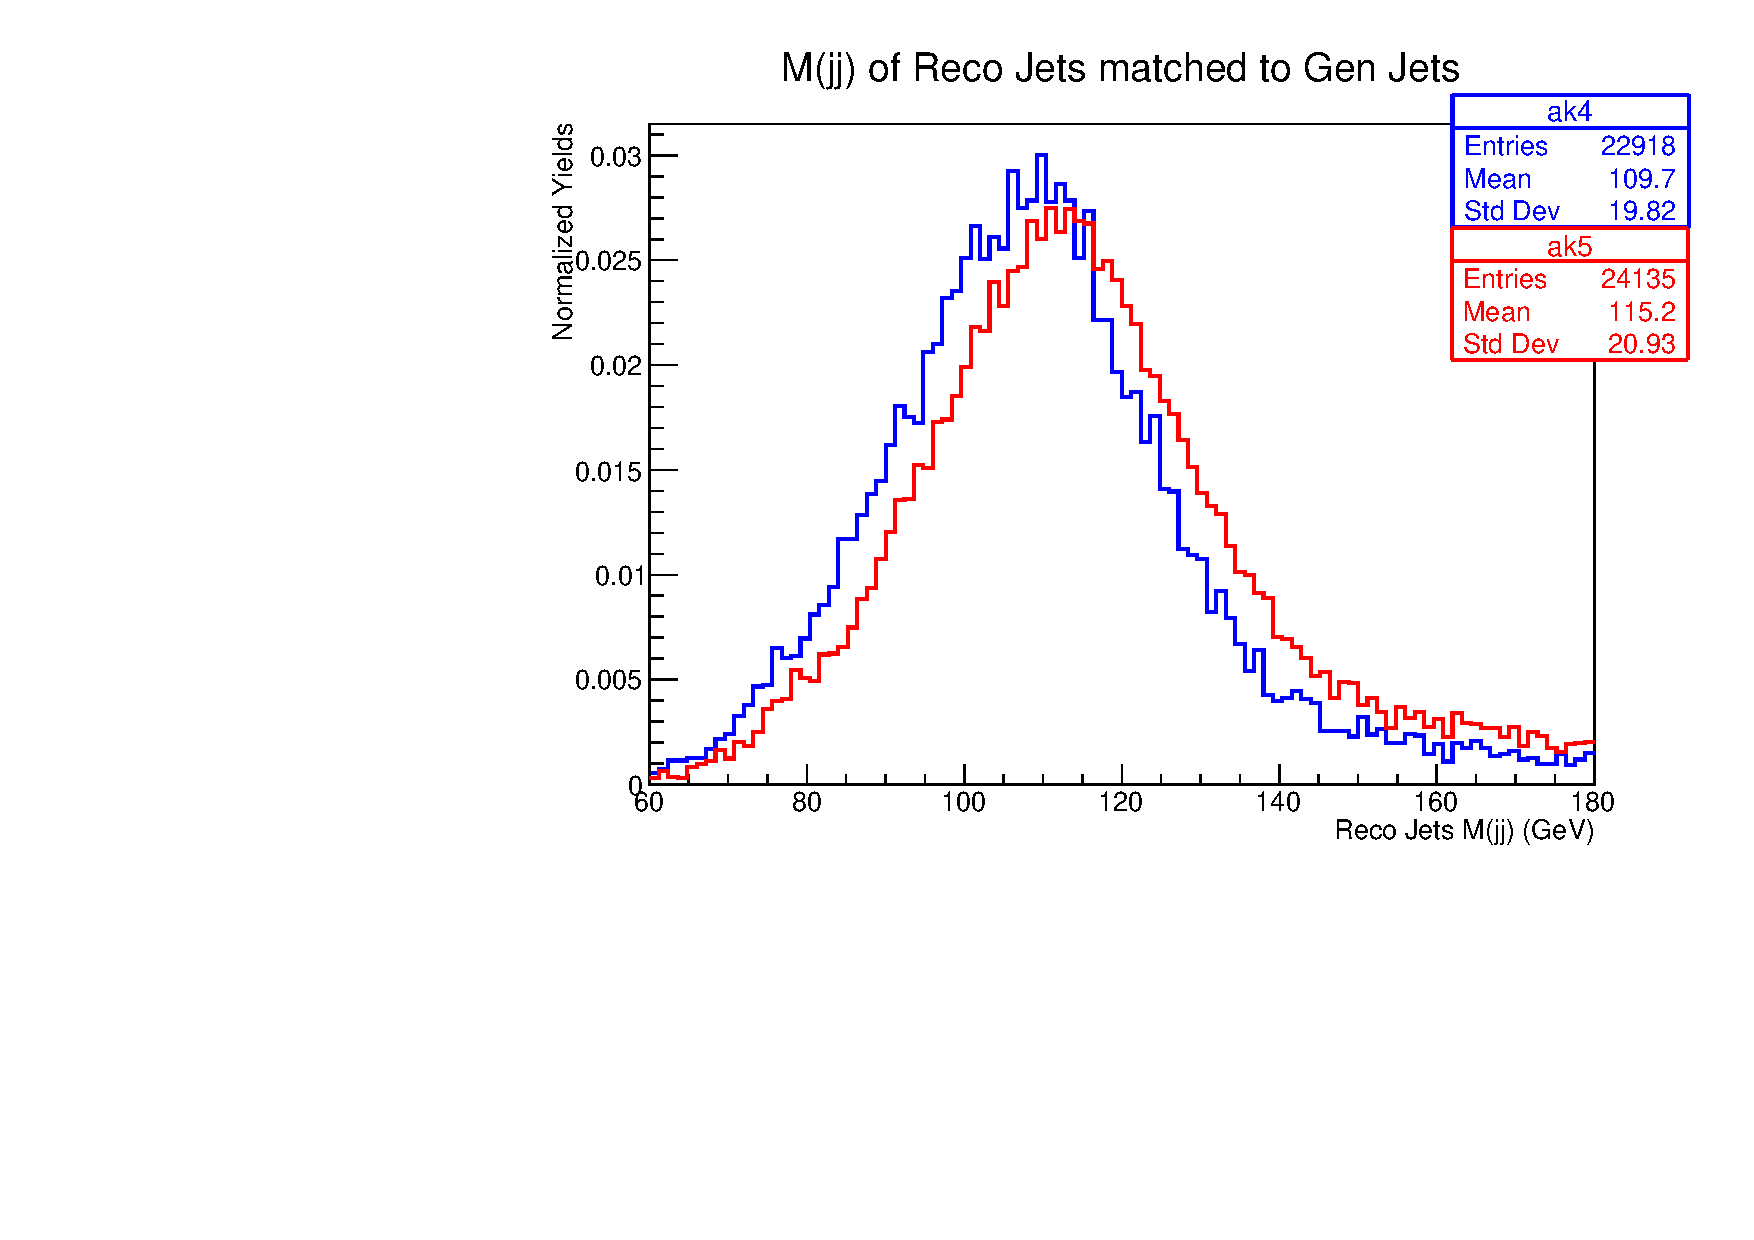
\includegraphics[width=0.45\textwidth]{figures/sec-jets/jet_rec.pdf}\hfil
  \caption{Difference between jet reconstruction used in Run I (red) and Run II (blue)}
  \label{fig:jet-reco}
\end{figure*}

We use the \textit{Loose ID} criteria to select the jets, which is described in
Ref~\cite{jetID-twiki}.

The jet candidates in the event, after passing the aforementioned ID,
must have $\PT > 25 \gev$ and $|\eta| < 2.4$ (so that they are within
the tracker of CMS and can be tagged as coming from $b$ quark). The
jets must also be outside the photon cone with a $\Delta R(j,\gamma) >
0.4$. Dijet objects are then created and only dijets with $\Mjj$ between 60 and 180 GeV 
pass the selection. If more than one dijet has passed those criteria, the dijet with two jets
with highest b-tagging score (see sec. \ref{sec:btag}) are selected as
the dijet candidate.


\subsection{Jet energy regression}
\label{sec:b-reg}

In addition to the misfortune of a small distance parameter of the jet reconstruction algorithm, the energy of the jets coming from $b$-quarks can not be fully reconstructed due to neutrinos escaping the detector. 
In order to improve the \Mjj resolution and gain in S/B discrimination, we employ an energy regression technique on our signal jets. 
The regression technique will work by changing the jet 4-momentum based on the likelihood that this specific jet is a signal jet. 

We use the TMVA package to implement the regression, and it on $X\to\HH\to\bbbb$ MC samples, in order to ensure a statistically independent training. 
Input variables to the training include jet kinematics, energy deposited in the calorimeter, vertex information, and variables related to missing transverse energy of the event (MET) and the distance between the two jets, $\Delta R(j,j)$. 
A summary of all input variables is shown in Table~\ref{tab:reg-vars}.

\begin{table}[h]\centering
\begin{tabular}{rl}
\hline
Input variables        & Jet kinematics: $\eta$, $\PT$, $m_T$\\
as in $\Hbb$ analysis  & Neutral hadron energy fraction, Photon energy fraction\\
regression:       & SecVtxdL, SecVtxdeL, SecVtxPt, SecVtxM, SecVtxNtrk\\
                  & Soft Lepton: \PT, \PT(rel), \DR \\
                  & \PT(Lead Track), Number of verteces\\\hline
\hline
Additional         & \\
variables for our  &\MET, $\Delta\phi(Jet, \MET)$, $\Delta R$(Leading jet, Trailing jet) \\
analysis:          & \\
\hline
\end{tabular}
\caption{Input variables used in TMVA regression. Upper part lists the
  variables that are also used in $\Hbb$ analysis, and the lower part
  lists additional variables.}
\label{tab:reg-vars}
\end{table}

The target for the regression training is $\PT^{gen}/\PT^{reco}$, where the generated level jet ("gen") contains neutrinos. 
This means that the regression technique will aim to construct, in a piece-wise manner, a function $f(\bar{x}) = \langle \PT^{gen}/\PT^{reco} \rangle (\bar{x})$, where $\bar{x}$ are the regression input variables, which can be used to correct the jet's energy. 
The standard gen-jet collection in CMS does not include the neutrinos, so we add them manually from gen-particle collection, using $\DR$ cone of 0.4 for matching.

Adding neutrinos to the gen-jet brings the energy of the jet closer to the energy of original b-quark, which is illustrated in Fig.~\ref{fig:b-reg-quark}.  
Figure~\ref{fig:b-reg-quark} also shows additional distributions, also comparing the gen-jets with and without
neutrino additions: \PT of the leading and trailing jets, invariant mass of the Higgs boson candidates and the $m_{jjjj}$. 
Events from all mass samples are combined, which explains the shape of $m_{jjjj}$ distribution. 
From these figures one can see the effects on the mass resolution of adding neutrinos to gen-jets.

\begin{figure*}[h]
  \centering
  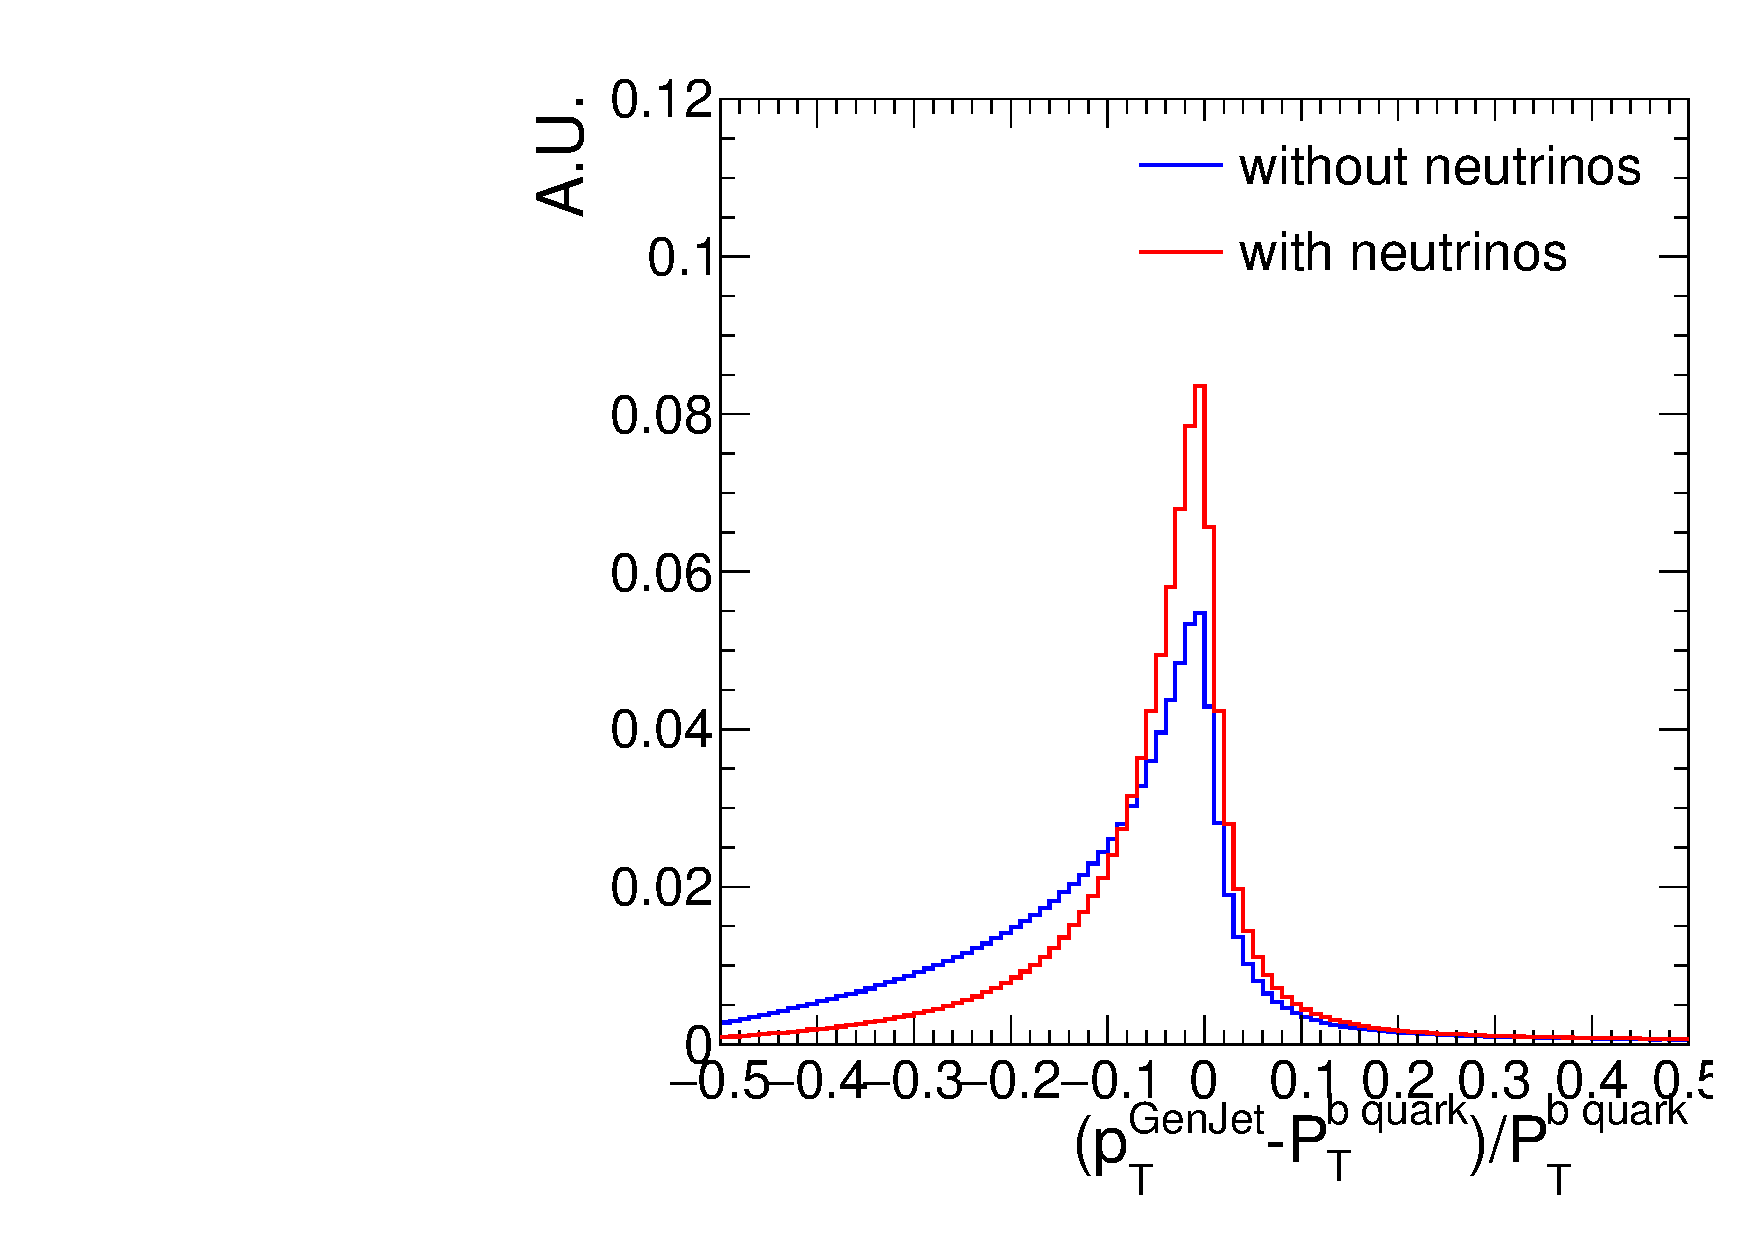
\includegraphics[width=0.33\textwidth]{b-reg/input_noBins_GenJetPtGenPtRel}\hfil
  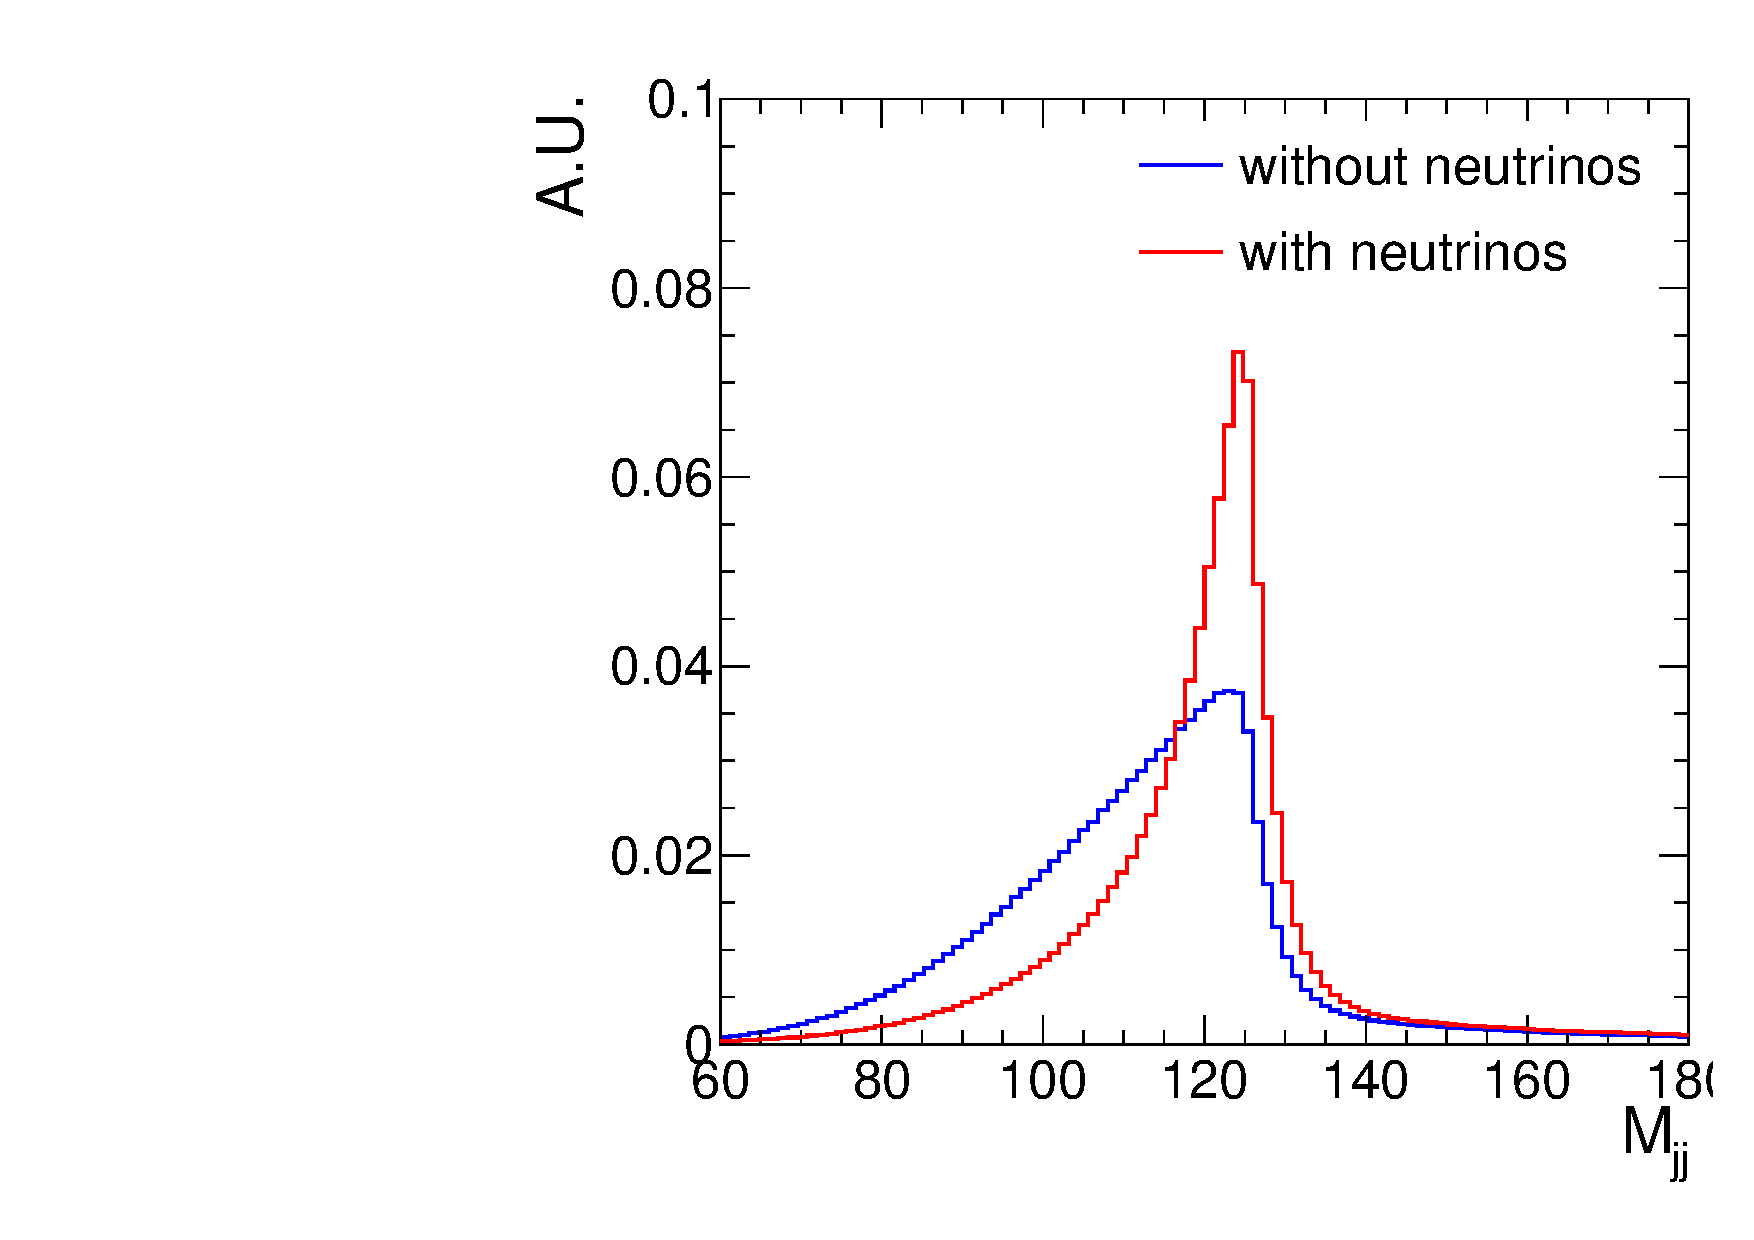
\includegraphics[width=0.33\textwidth]{b-reg/input_noBins_jjMass_Jetgenjet}\hfil
  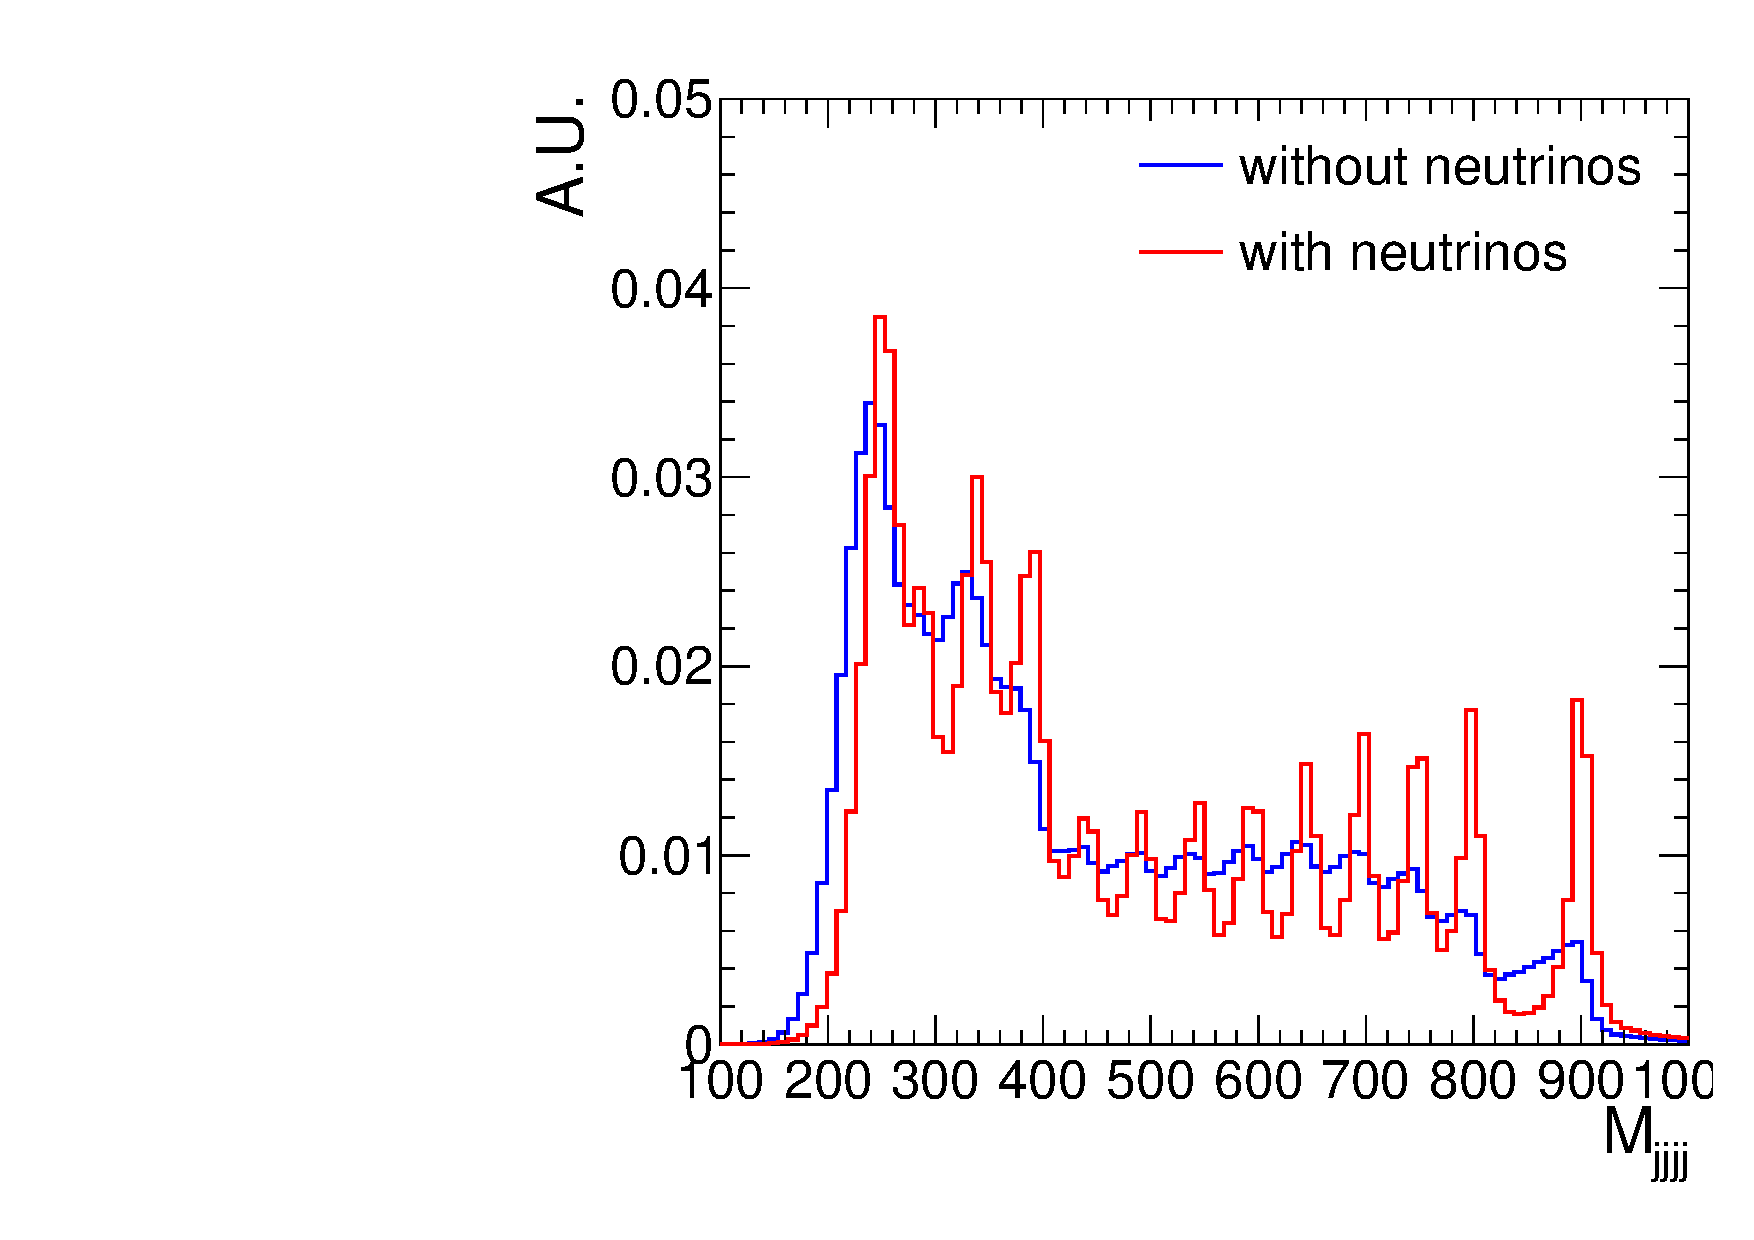
\includegraphics[width=0.33\textwidth]{b-reg/input_noBins_jjjjMass_Jetgenjet}\hfil

  \caption{Relative \PT difference, $m_{jj}$ and $m_{jjjj}$ distributions of the b-quark and the
    corresponding gen-jet, obtained from $\HH\to\bbbb$ samples. Red
    histogram is for gen-jets containing neutrinos, blue is for jets
    without neutrinos.}
  \label{fig:b-reg-quark}
\end{figure*}

For the training we select jets that satisfy the following criteria:
\begin{itemize}
\item $\PT > 20\GeV$, $|\eta| < 2.4$
\item Matched to the generated level jet within a cone $\DR<0.4$ (this matching is done as part of MiniAOD reconstruction)
\item Matched to a b-quark within a cone $\DR<0.4$
\end{itemize}


We perform six different trainings to check the impact of additional variables:
\begin{itemize}
\item Using 15 variables based on $\Hbb$ training, listed in
  Table~\ref{tab:reg-vars}. It is denoted as \textbf{Baseline} on the
  figures below.
\item Using 15 variables plus \MET and $\Delta\phi(Jet, \MET)$.
\item Using 15 variables plus \MET , $\Delta\phi(Jet, \MET)$, and also
  $\Delta R$(Leading jet, Trailing jet).  This training is denoted as
  \textbf{full 15+3var} in the text.
\item Using 15 variables as above but in addition, for each pair of
  jets from the Higgs boson, the training is performed separately for
  the leading and trailing jets. That is, two XML weight files are
  derived, one for the leading and one for the trailing jet in the
  event.  This method is denoted as \textbf{js} on the figures and in
  the text.
\item Using 15 plus \MET and $\Delta\phi(Jet, \MET)$ variables, and
  separating the training for leading and trailing jets as above.
\item Using 15 plus \MET, $\Delta\phi(Jet, \MET)$ and $\Delta R$
  variables, and separating the training for leading and trailing jets
  as above.
\end{itemize}

The regression is performed with the TMVA package, using the Boosted Decision Tree technique with gradient boosting. 500 decision trees with depth 5 are created to estimate the target. 
The pruning technique is applied.
The detailed TMVA modified options are as follows:

\verb|NTrees=500:MaxDepth=5:nCuts=500:BoostType=Grad:!UseBaggedGrad|

\verb|Shrinkage=0.1:MinNodeSize=1:PruneStrength=5:PruneMethod=CostComplexity|

\verb|NegWeightTreatment=IgnoreNegWeightsInTraining|

After the training is done, its performance is checked in signal samples, $X\to\HH\to\ggbb$, at all mass points of $m_X$.  
The selection is the same as the training samples. 
All of our trainings are compared with the one done by $\Hbb$ analysis, which is denoted as \textbf{Hbb} on the figures. 
The $\PT^{reco}$ of the reconstructed jet can be compared to the target $\PT^{gen}$ of the generated jet with neutrinos. 
An example of such distributions is shown in Fig.~\ref{fig:b-reg-pt-res} for the leading and trailing jets. 
From distributions such as in Fig.~\ref{fig:b-reg-pt-res} we obtain the mean value for the \textbf{scale} and sigma ($\sigma$) for the \textbf{resolution}. 
The mean value and sigma are obtained from the Bukin function fit. 
The scale and resolution of the leading and trailing jets versus their \PT are shown in Fig.~\ref{fig:b-reg-jet-res}. 
From this figure we can conclude that adding MET variables into the training improves significantly the resolution. 
As expected the \textbf{15+3var js} training gives best per-jet resolution across the whole \PT range.

\begin{figure*}[h]
  \centering
  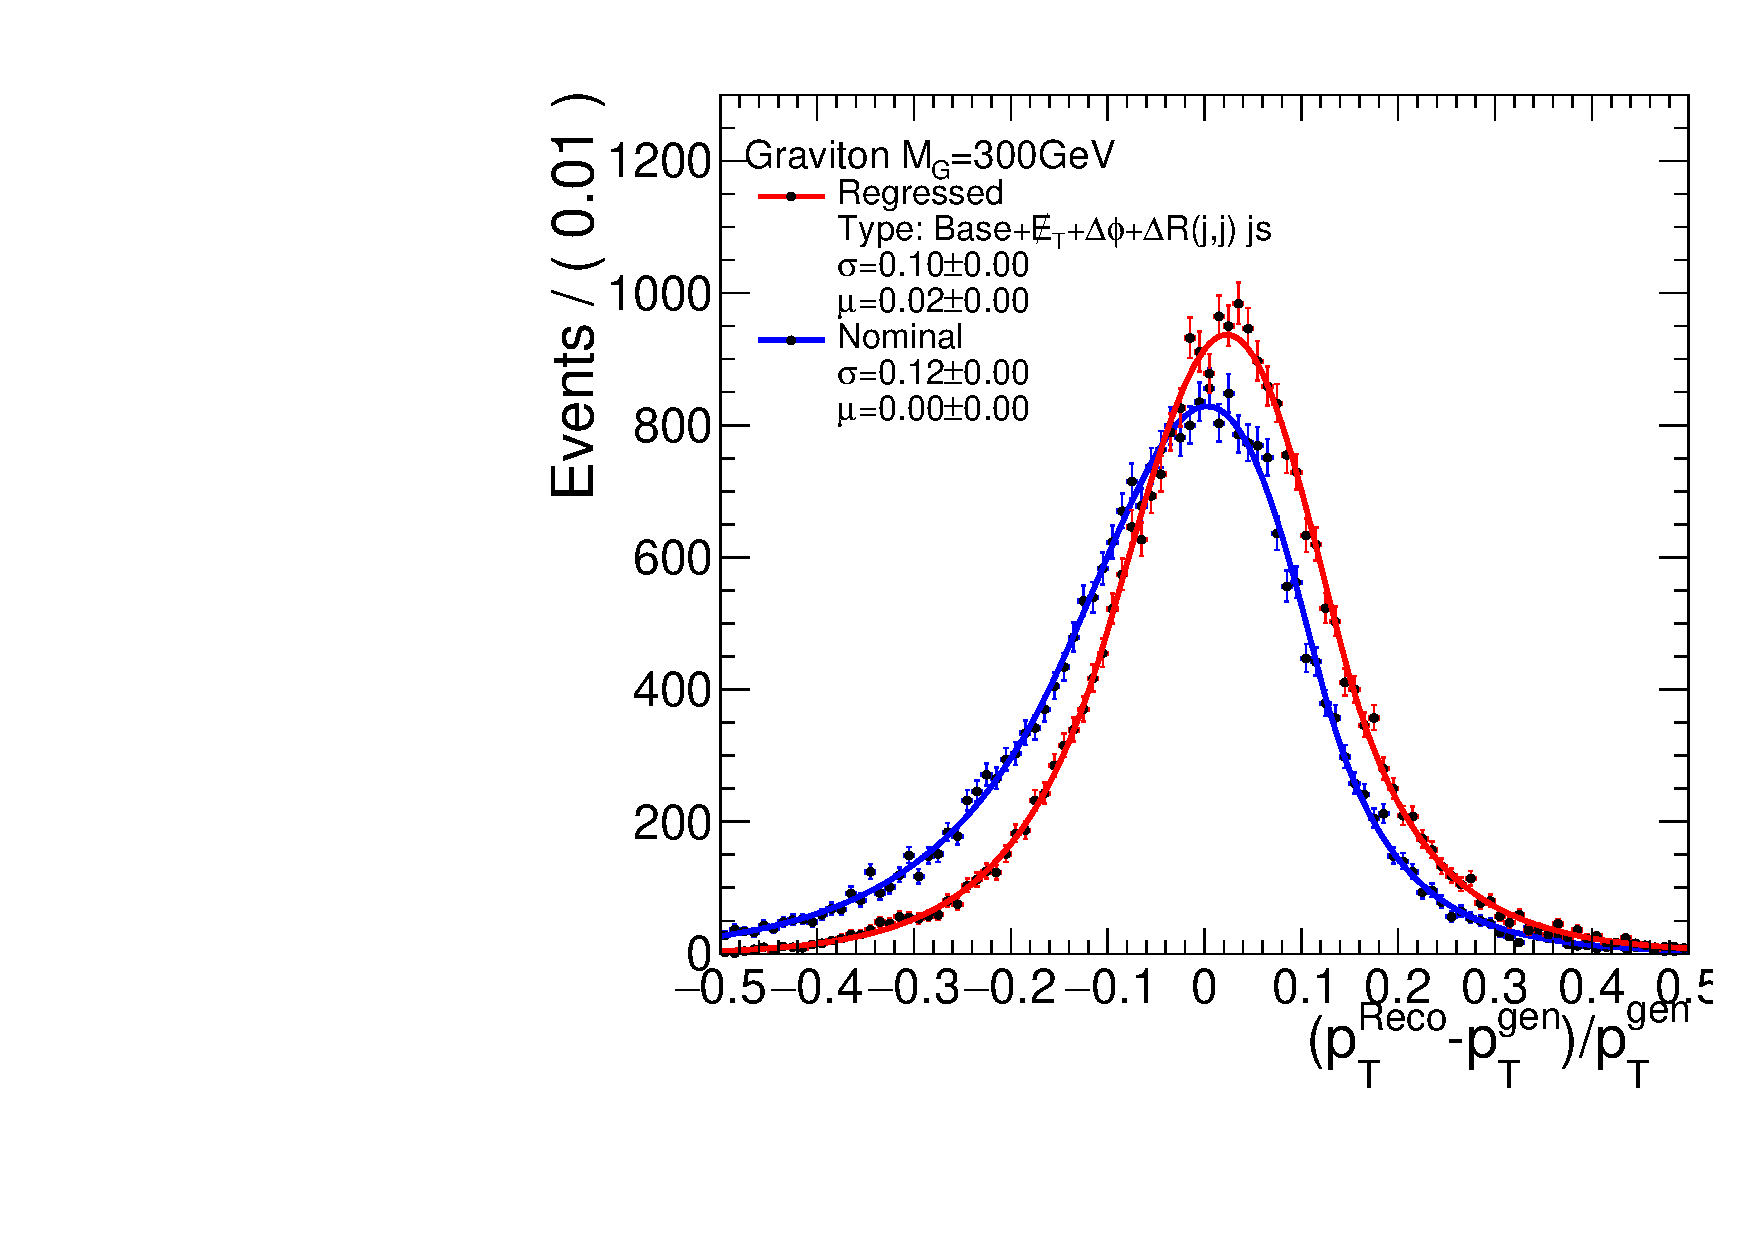
\includegraphics[width=0.35\textwidth]{b-reg/AN_mass300_J1}\hfil
  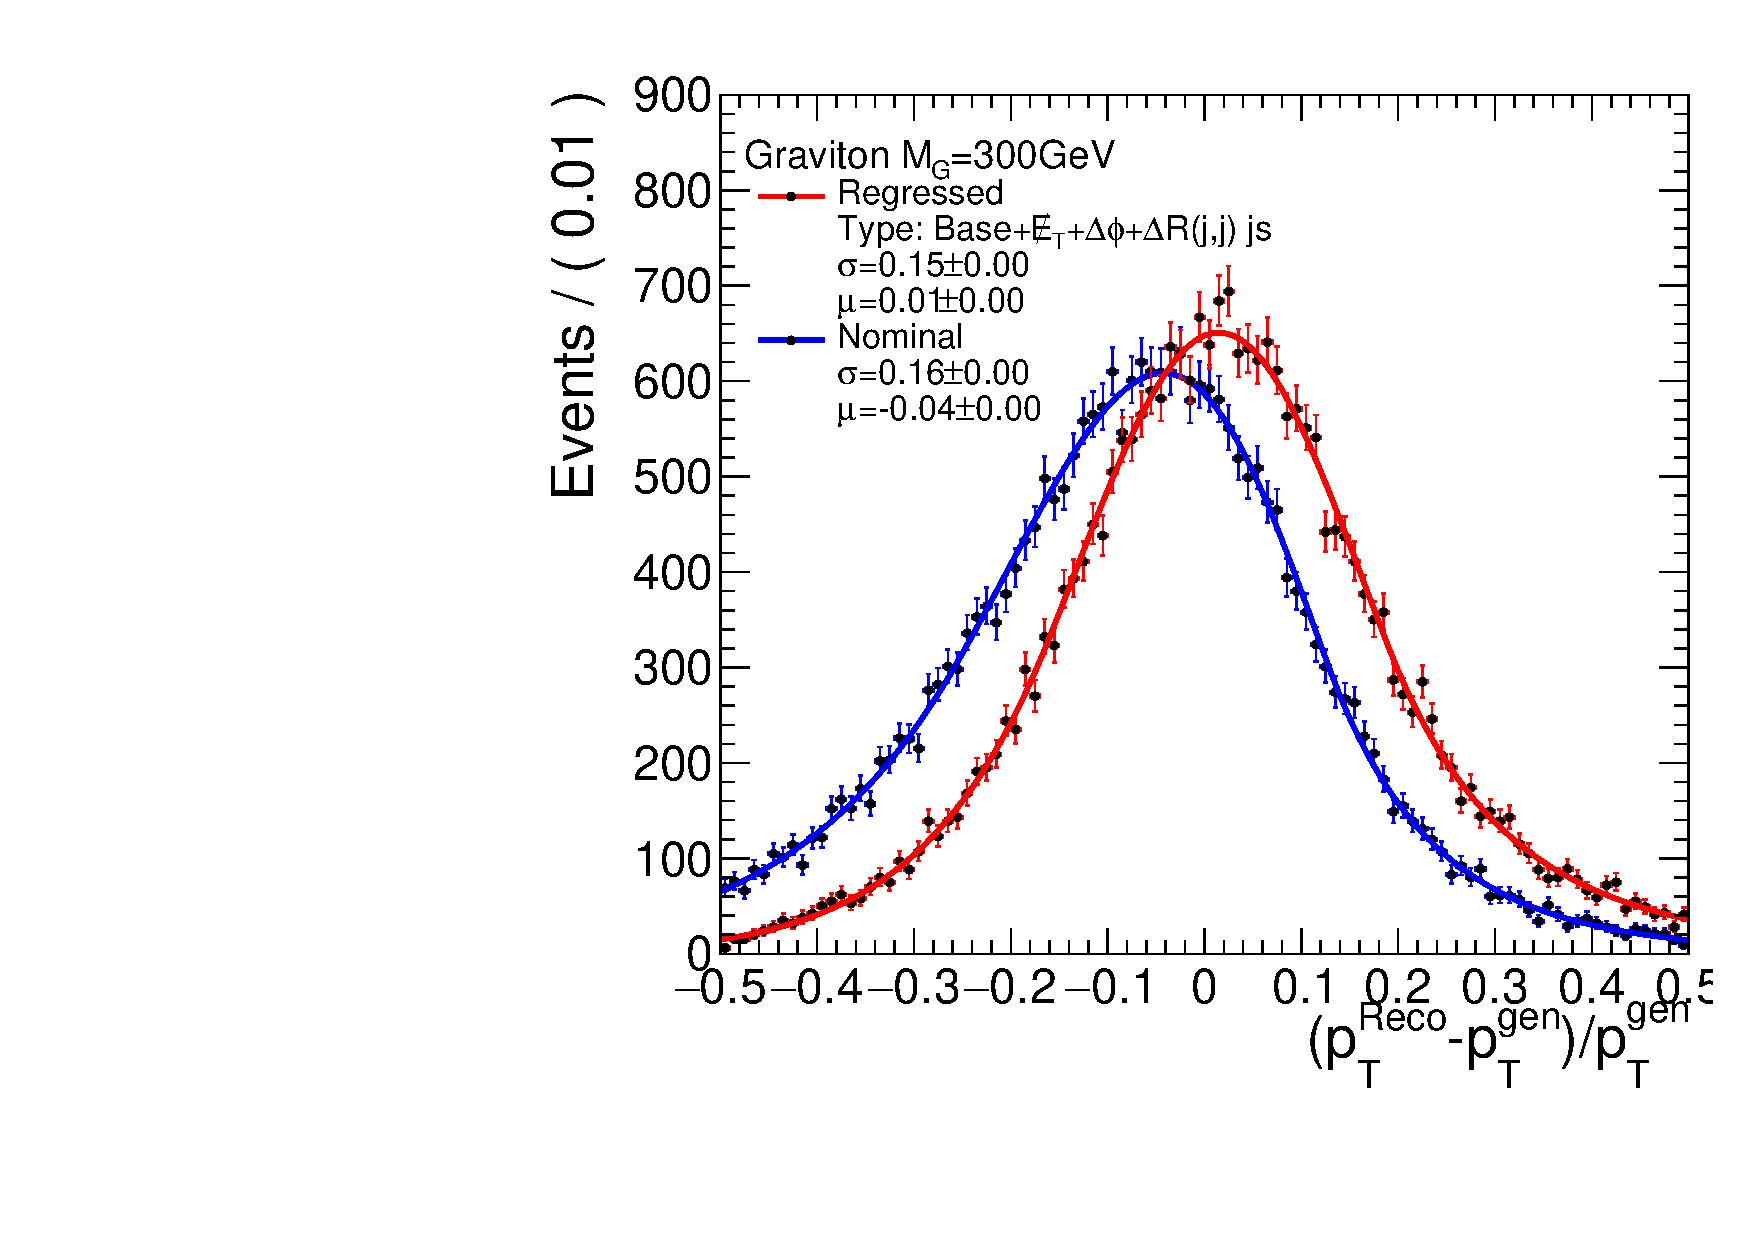
\includegraphics[width=0.35\textwidth]{b-reg/AN_mass300_J2}\hfil
  \caption{Relative \PT difference of the reconstructed and generated
    level jets after regression (red histograms) and without
    the regression (blue histograms).}
  \label{fig:b-reg-pt-res}
\end{figure*}

\begin{figure*}[h]
  \centering
  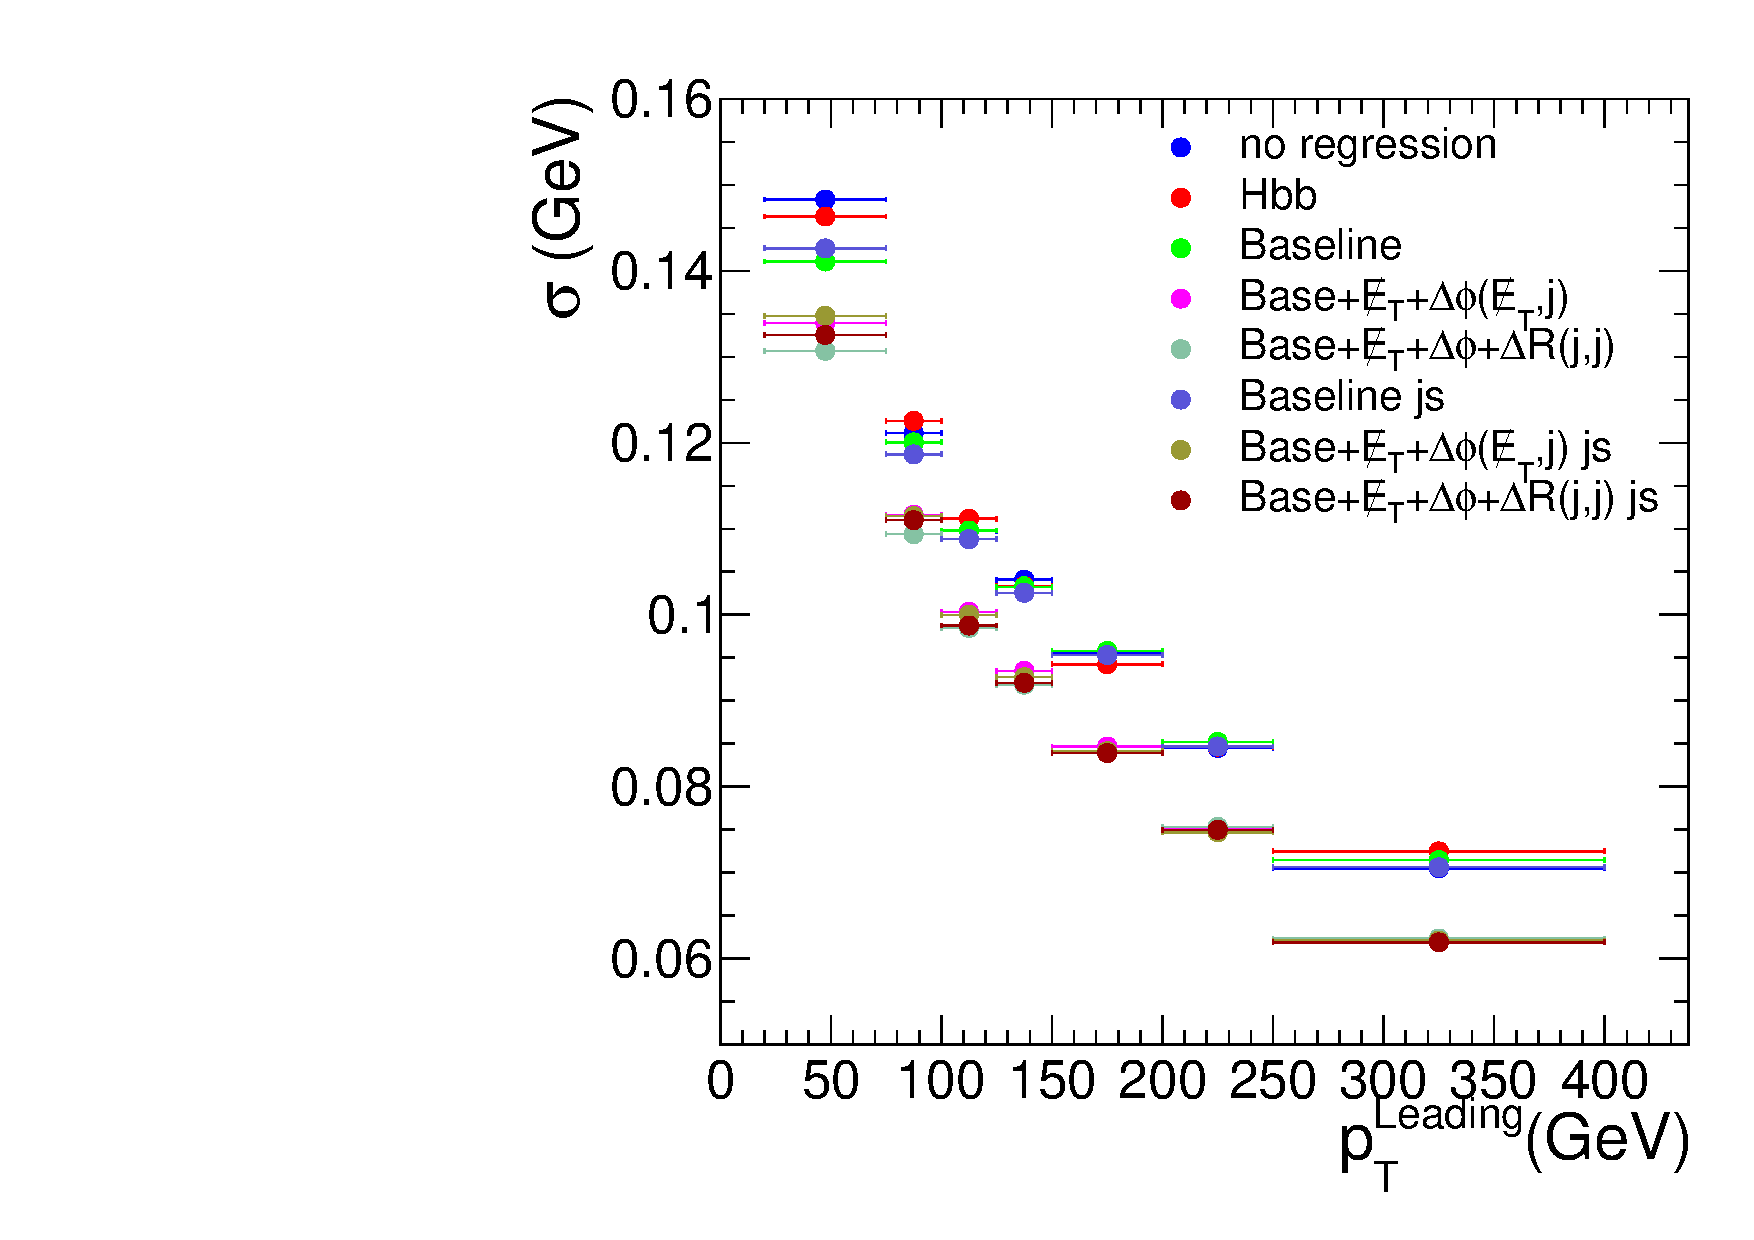
\includegraphics[width=0.35\textwidth]{b-reg/AN_HHbbgg_G_sigma_jet1pT}\hfil
  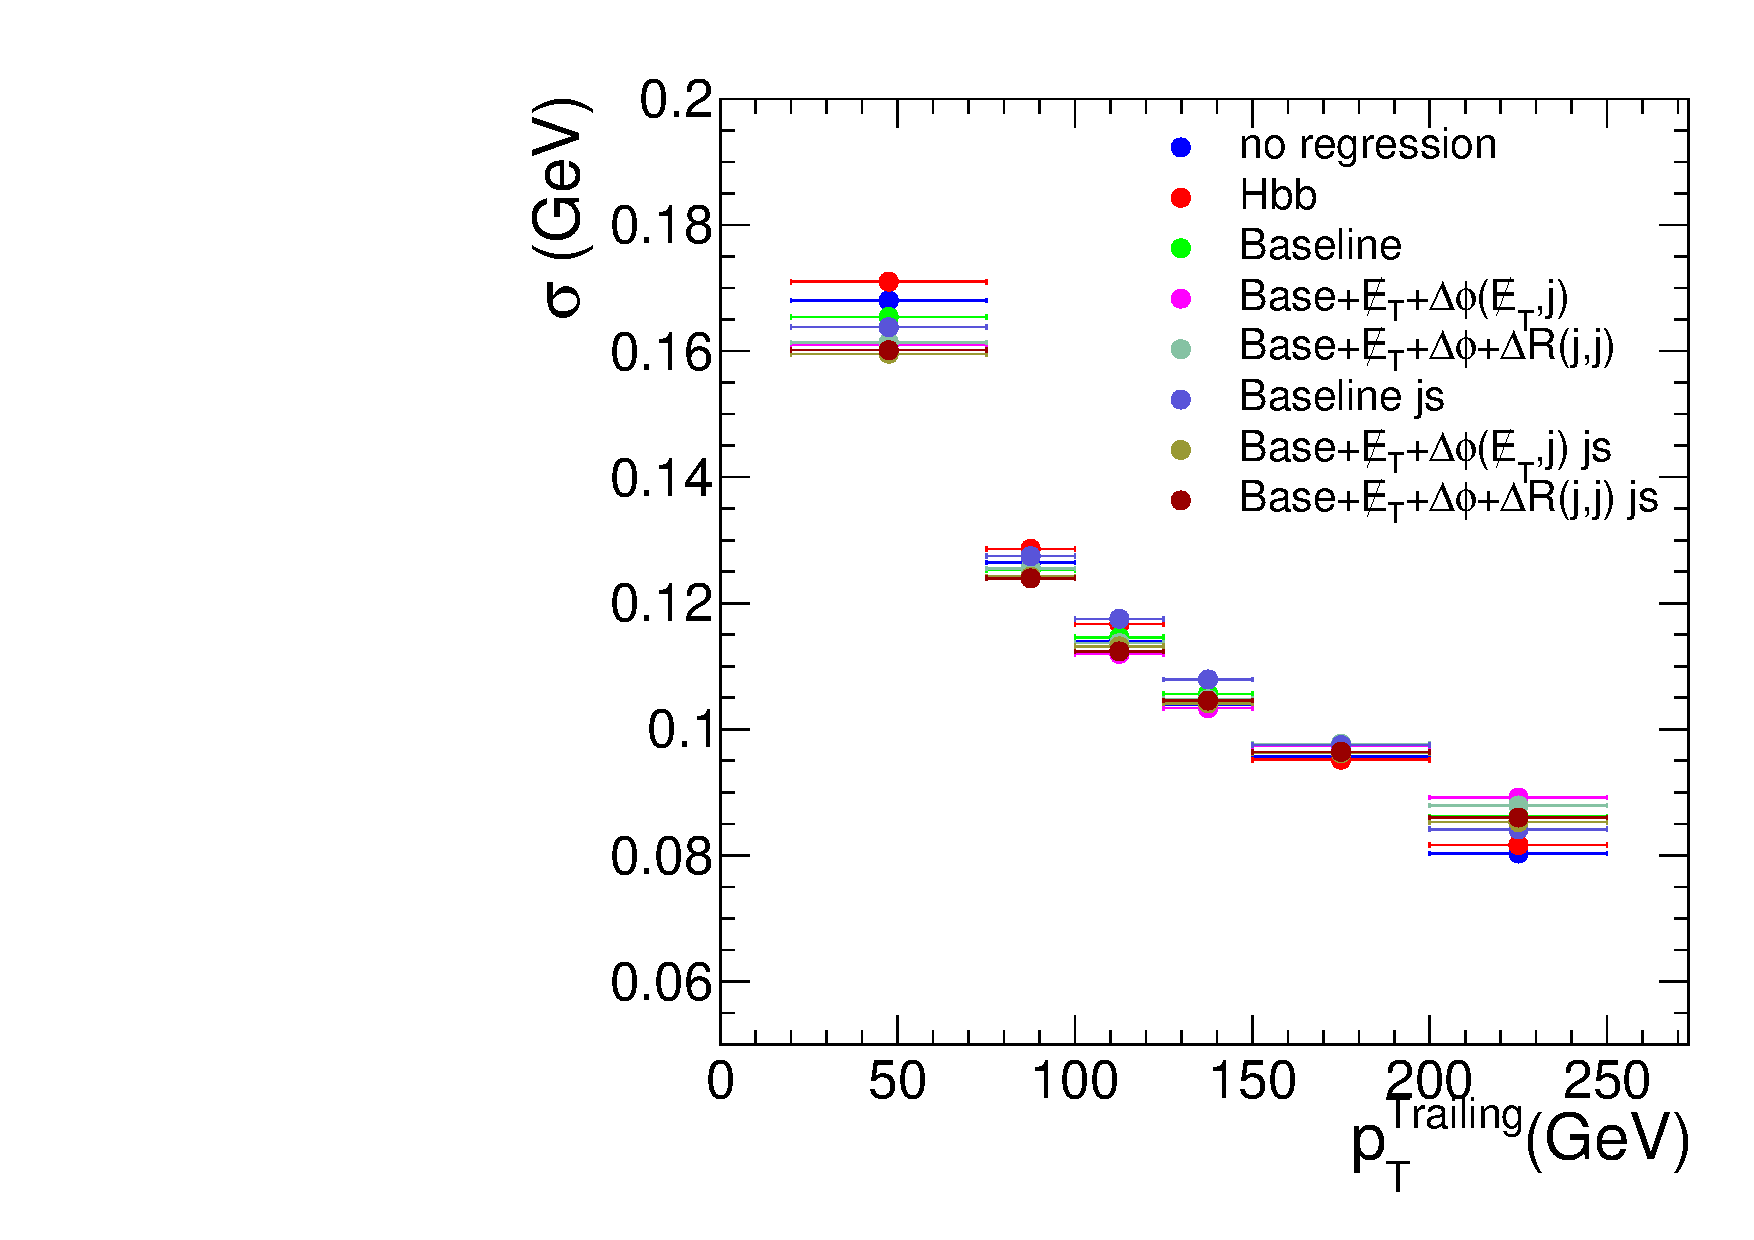
\includegraphics[width=0.35\textwidth]{b-reg/AN_HHbbgg_G_sigma_jet2pT}\hfil\\
  \caption{The resolution of the jet \PT for leading (left) and trailing (right) jets from the signal
    sample $G\to\HH\to\ggbb$.}
  \label{fig:b-reg-jet-res}
\end{figure*}
  
  \begin{figure*}[h]
  \centering
  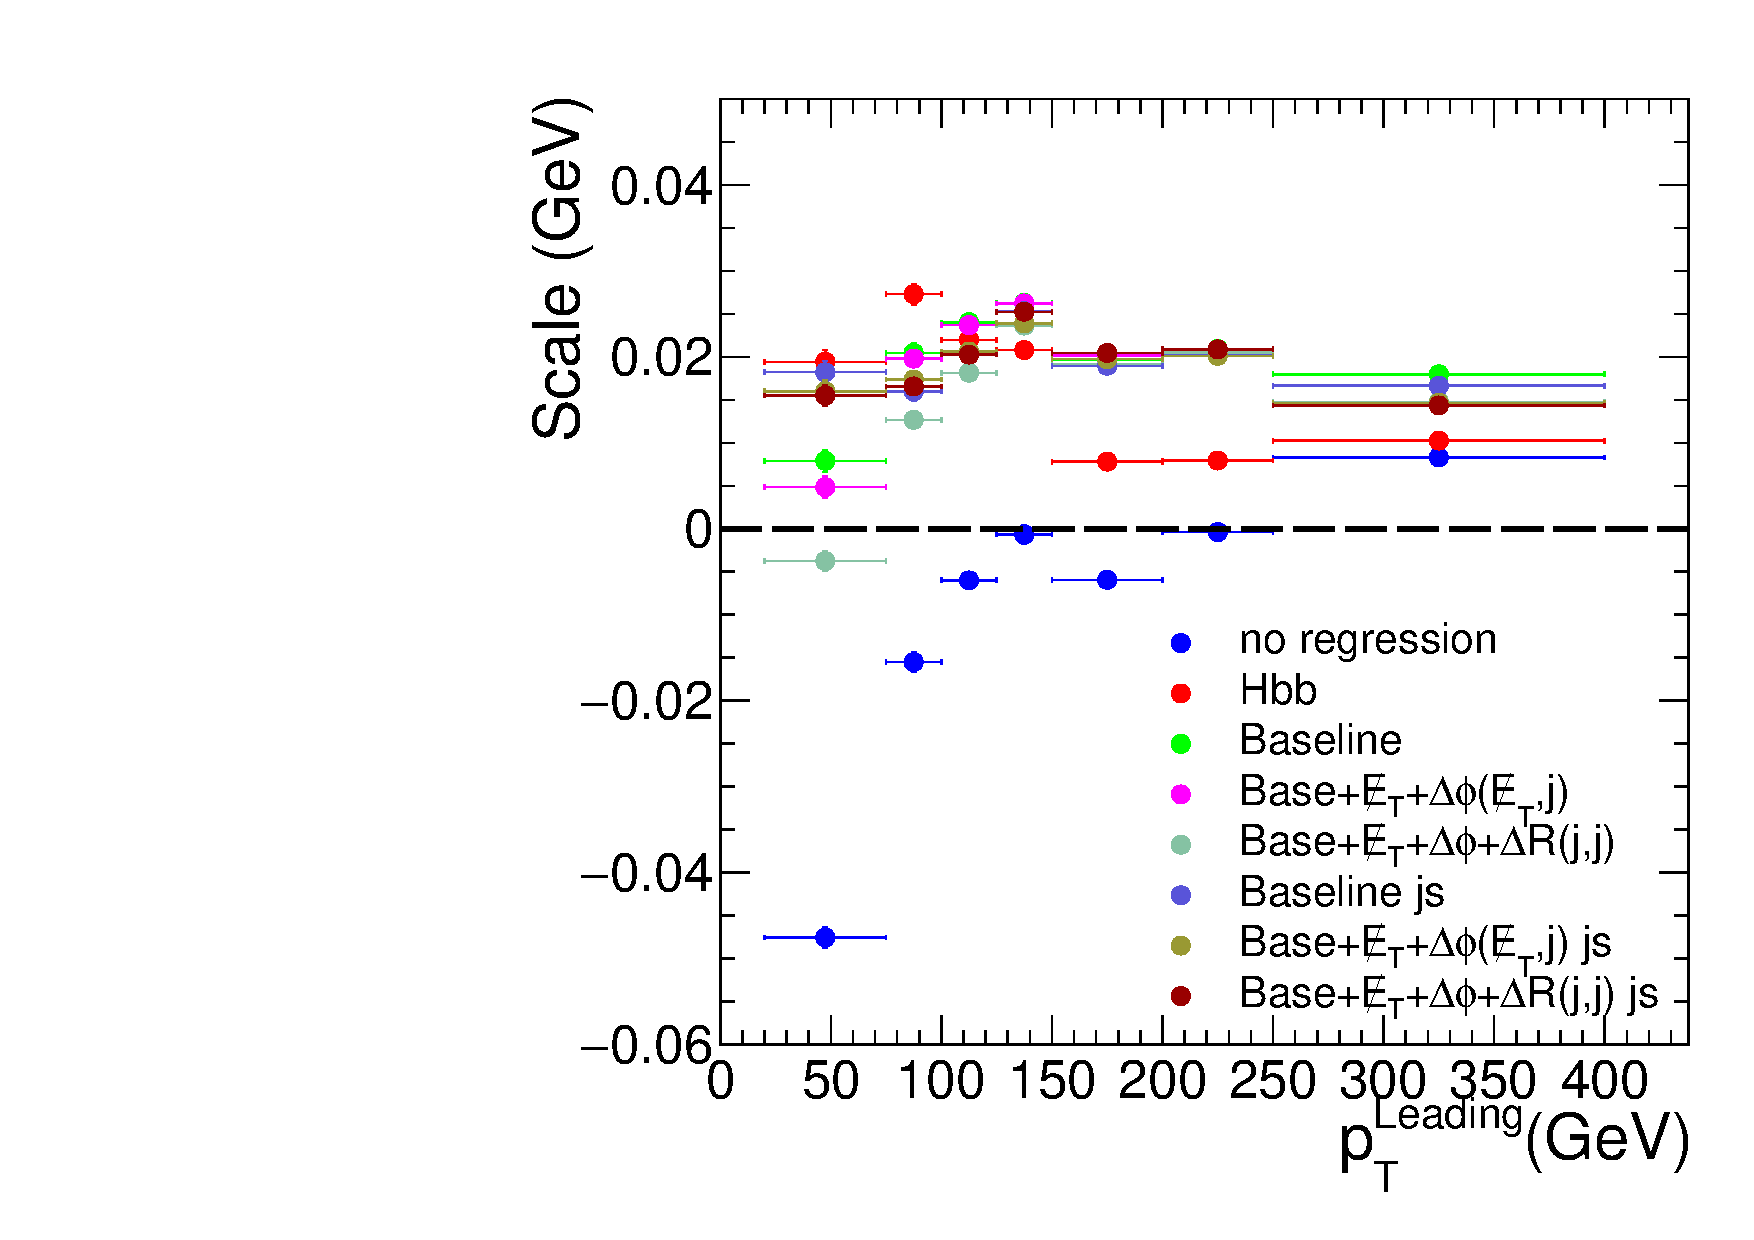
\includegraphics[width=0.35\textwidth]{b-reg/AN_HHbbgg_G_scale_jet1pT}\hfil
  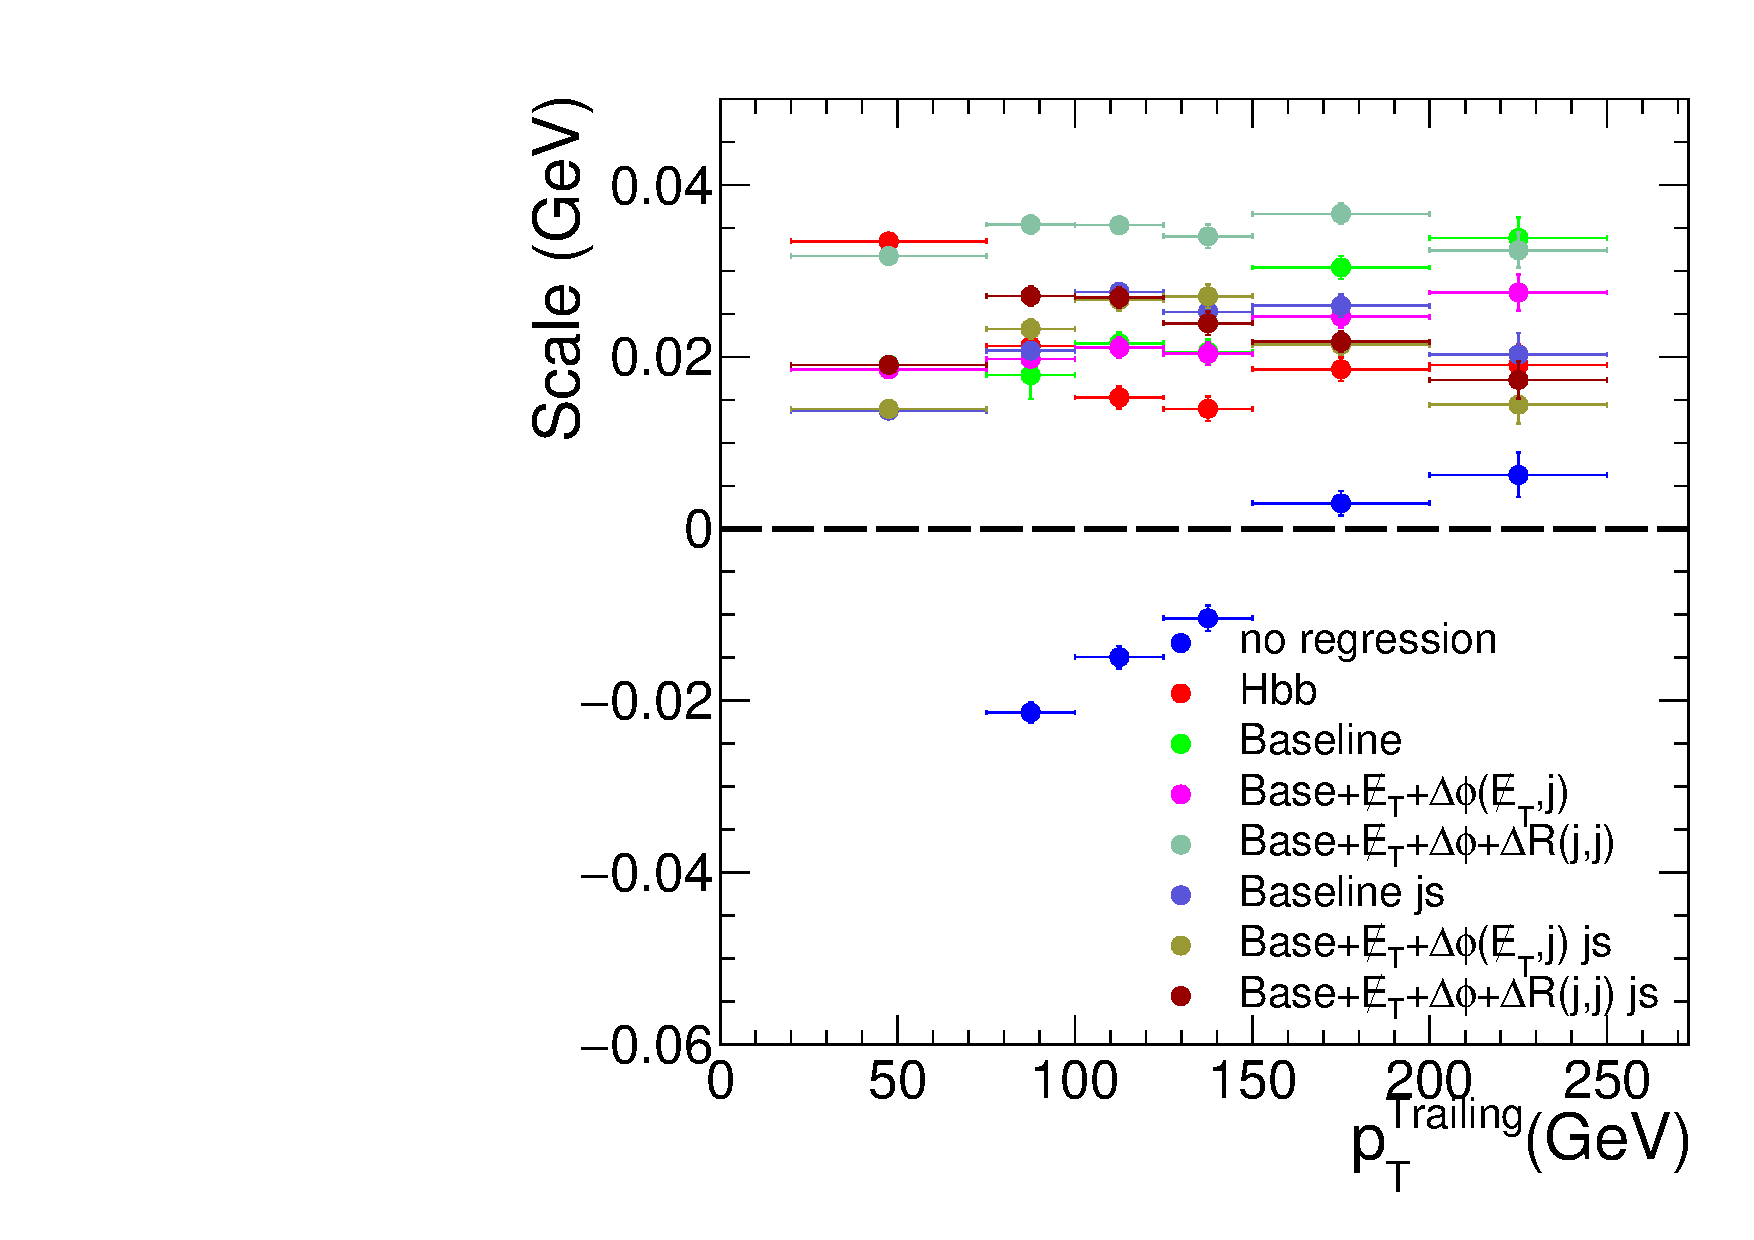
\includegraphics[width=0.35\textwidth]{b-reg/AN_HHbbgg_G_scale_jet2pT}\hfil\\
  \caption{The scale of the jet \PT for leading (left) and trailing (right) jets from the signal
    sample $G\to\HH\to\ggbb$.}
  \label{fig:b-reg-jet-scale}
\end{figure*}

The purpose of the regression is to improve the Higgs boson mass resolution from the $\Hbb$ decay in $X\to\HH\to\ggbb$ signal.  
The distributions together with the fit by Bukin function are shown in Figs.~\ref{fig:b-reg-mH-fit-reco}, where the reconstructed mass is shown after the \textbf{full 15+3var js} regression training, for $m_G = 300\GeV$ and $m_G = 900\GeV$.

After the fitting to the corresponding function is done, we obtain the mean and the width parameters of the fit.  
The width and mean (both in \GeV) are shown on Fig.~\ref{fig:b-reg-mH-res} versus the mass of the Graviton particle.  
From this figure we arrive at the same conclusion  as for single-jet plots of Fig.~\ref{fig:b-reg-jet-res}: the MET variables improve the resolution and the \textbf{full 15+3var js} training gives the best mass resolution. 
The training with \textbf{15} variables give similar results to the \textbf{Hbb} training.  
In all trainings the scale does not match the nominal value of the Higgs boson mass. 
This is expected because the jets (both at reco and gen levels) do not contain the whole energy of the Higgs boson decay.

\begin{figure*}[h]
  \centering
  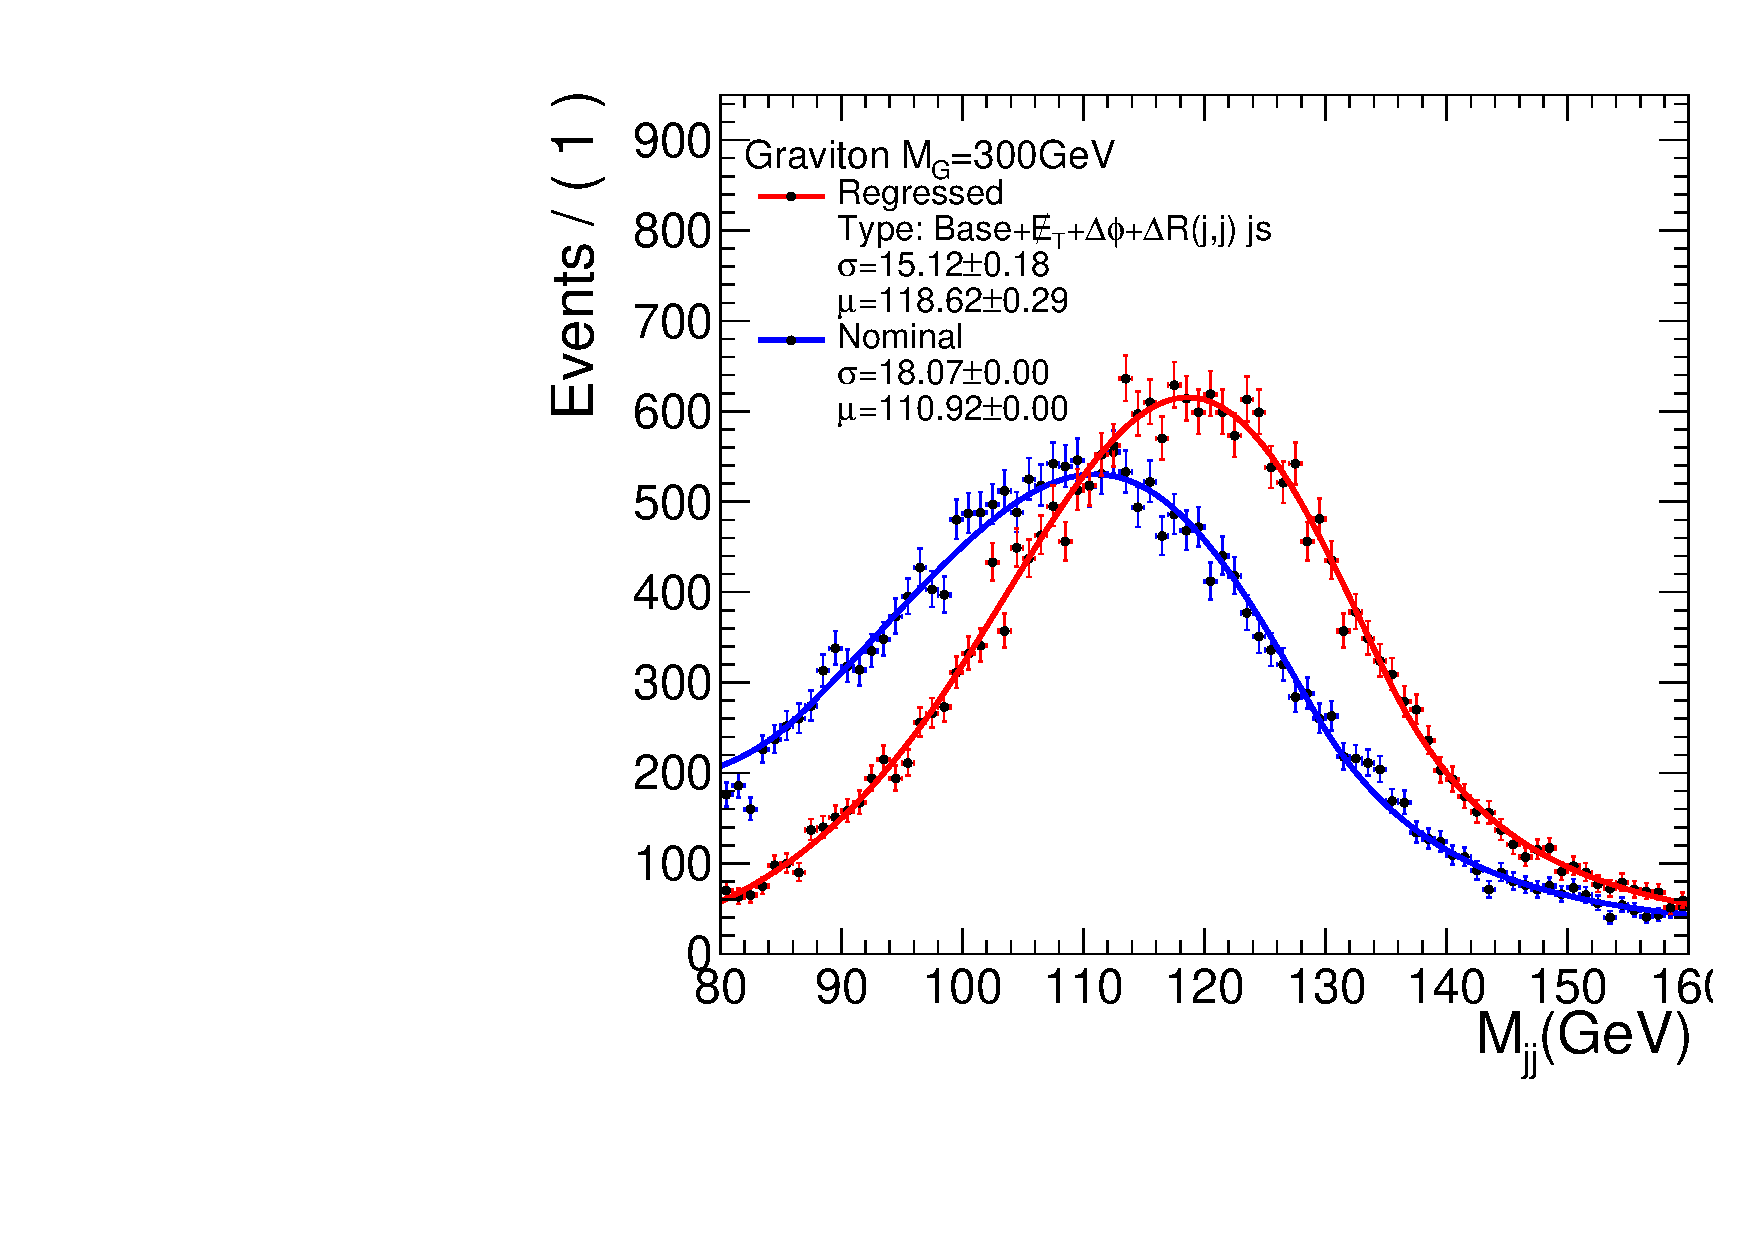
\includegraphics[width=0.35\textwidth]{b-reg/AN_mass300}\hfil
  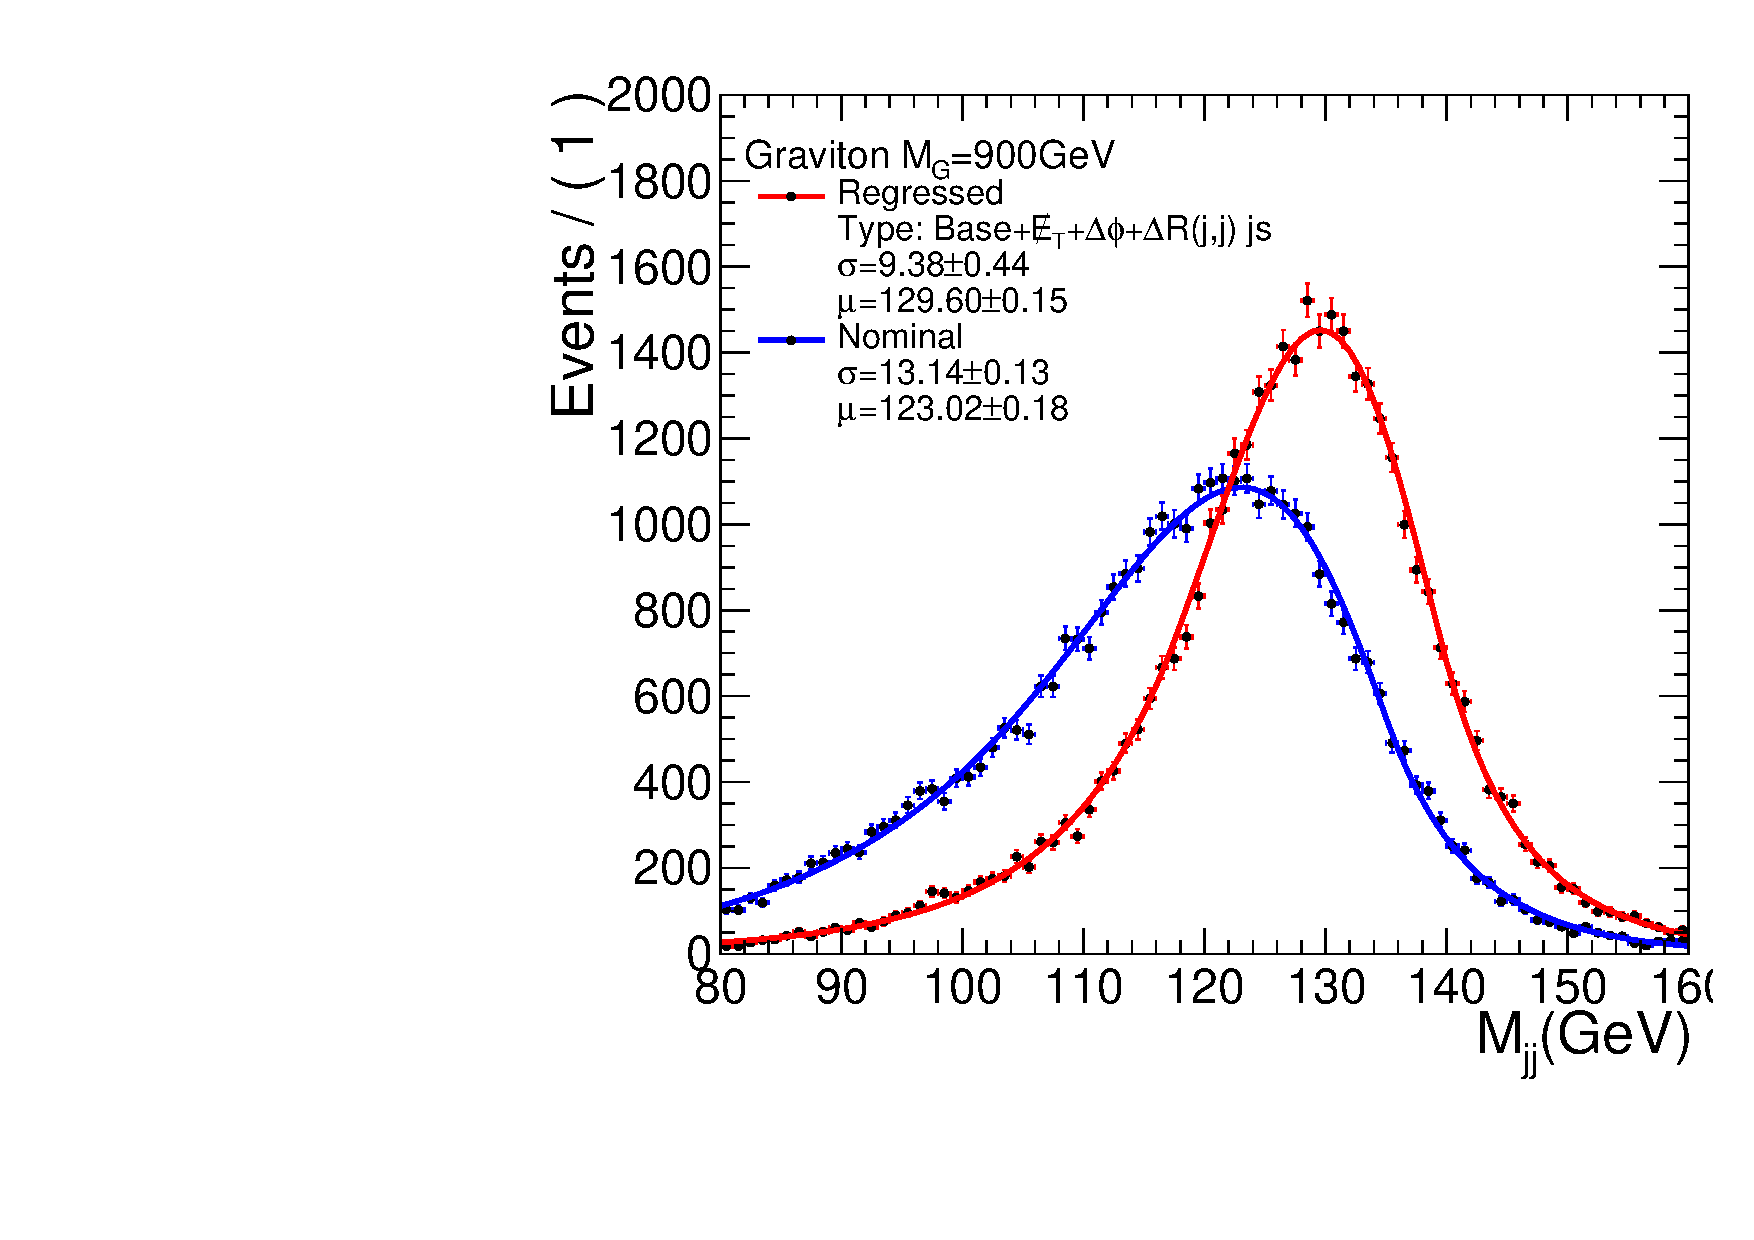
\includegraphics[width=0.35\textwidth]{b-reg/AN_mass900}\hfil
  \caption{$M_{jj}$ distributions from the reco-jets before and after
    the \textbf{full variables with js} regression for $m_G=300\GeV$ signal sample
    (left) and $m_G=900\GeV$ signal sample (right).}
  \label{fig:b-reg-mH-fit-reco}
\end{figure*}

\begin{figure*}[h]
  \centering
  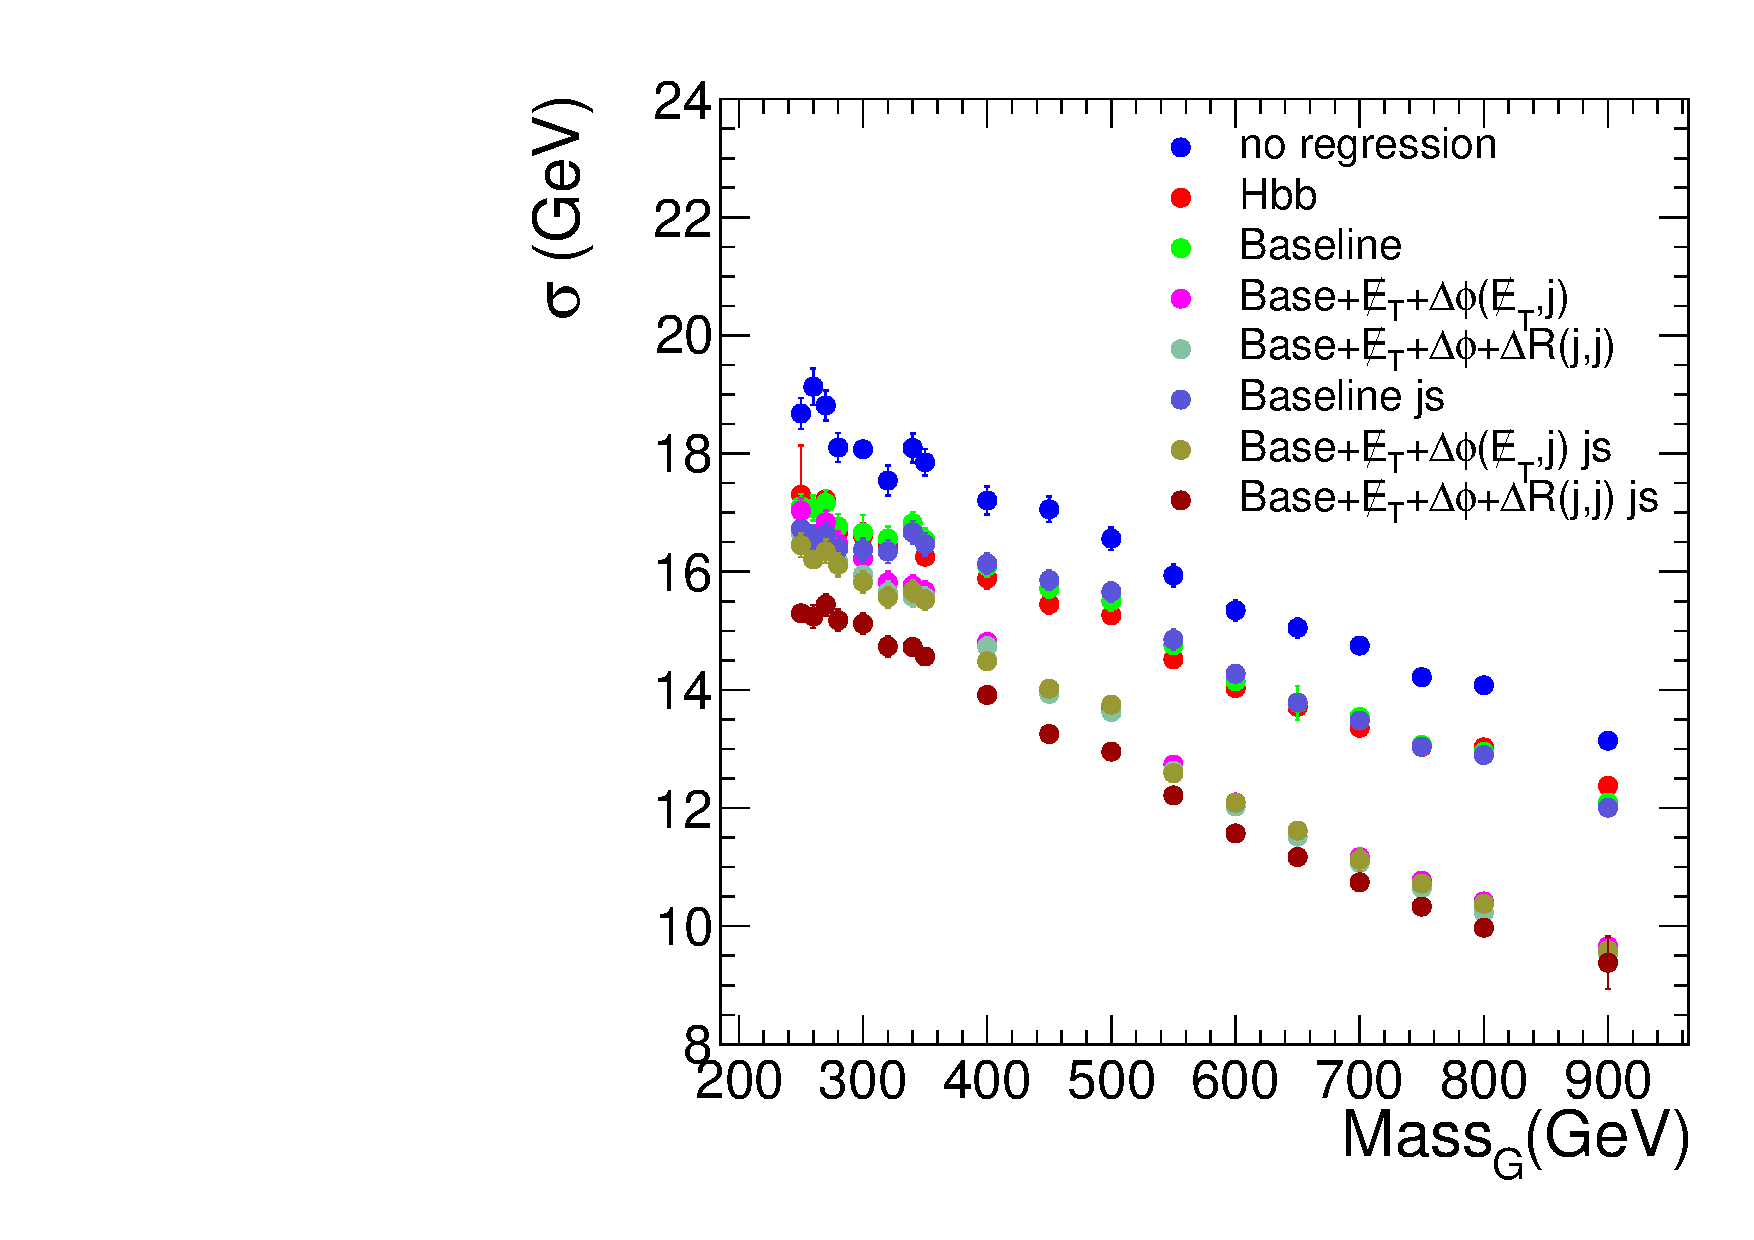
\includegraphics[width=0.35\textwidth]{b-reg/AN_HHbbgg_G_sigma_Mass}\hfil
  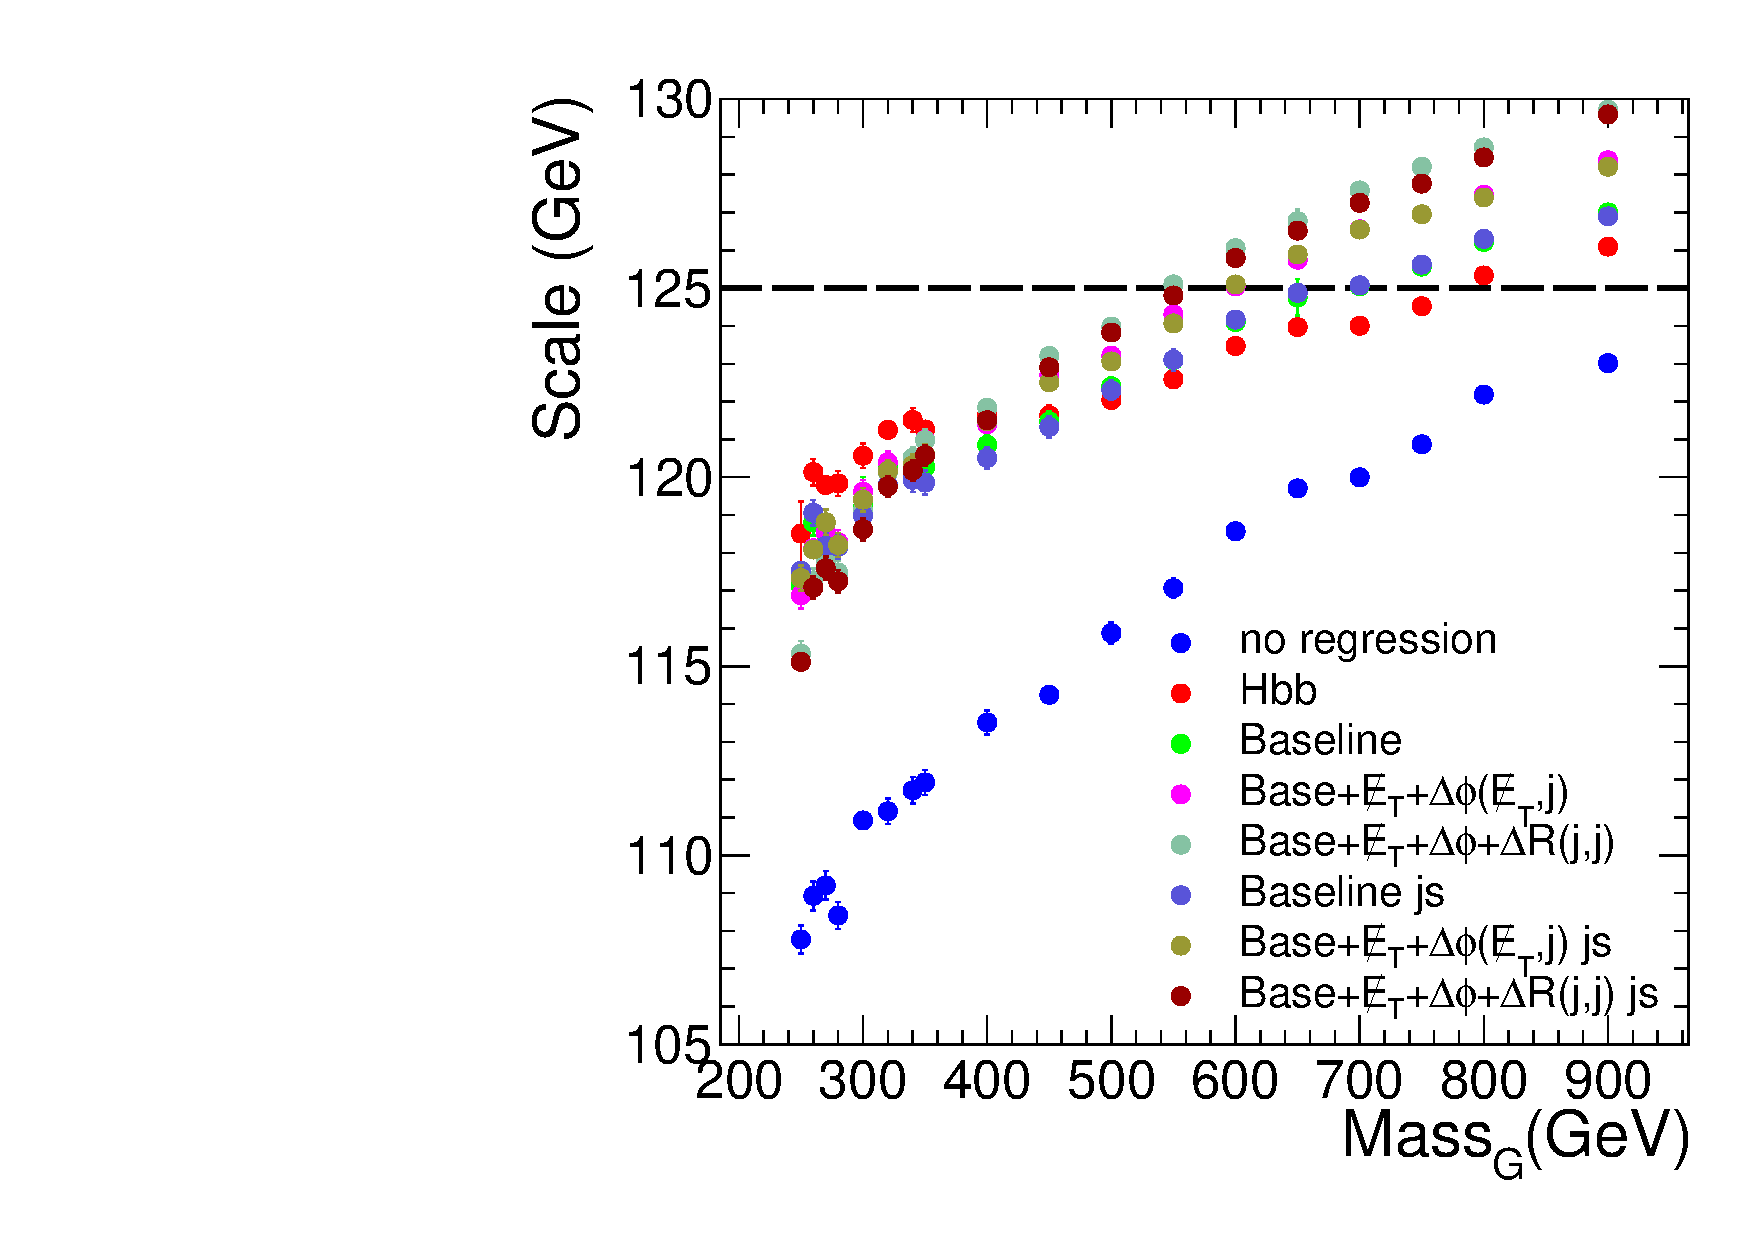
\includegraphics[width=0.35\textwidth]{b-reg/AN_HHbbgg_G_scale_Mass}\hfil
  \caption{Performance plot comparing different regression trainings.}
  \label{fig:b-reg-mH-res}
\end{figure*}


In order to validate the developed regression in data we select events with $\Z\to\ell\ell$ decay which also contain two b-tagged jets. 
It is assumed that a di-jet is recoiled against $\Z$ boson, and therefore the $\PT(jj)$ must balance the $\PT(\ell\ell)$.  
This check was done both in muon and electron channels of \Z boson decay, analyzing \verb|DoubleMuon| and \verb|DoubleElectron| datasets correspondingly, using 2016 data.

In the muon channel the events were selected with an OR of two triggers:
\begin{itemize}
\item \verb|HLT_Mu17_TrkIsoVVL_Mu8_TrkIsoVVL_DZ| and 
\item \verb|HLT_Mu17_TrkIsoVVL_TkMu8_TrkIsoVVL_DZ|. 
\end{itemize}
The reconstructed muons must pass Tight muon ID and Loose PF isolation. 

In the electron channel the \verb|HLT_Ele23_Ele12_CaloIdL_TrackIdL_IsoVL_DZ| trigger was used and
the electrons required to pass MVA ID WP90 selection.  
Further event selection requirements in both channels are: $\PT(\ell_1) > 25\GeV$,
$\PT(\ell_2) > 15\GeV$, $\PT(\ell\ell) > 50\GeV$,
$75<m_{\ell\ell}<105\GeV$, $\Delta R^{min}_{\ell, jet} > 0.4$. The two
jets in the event must pass Loose PF ID selection, Medium PU jet ID,
tagged as b-jets with CSVv2 Medium WP, and have $\PT>20\GeV$,
$|\eta|<2.4$.

\begin{figure*}[thb]
  \centering
  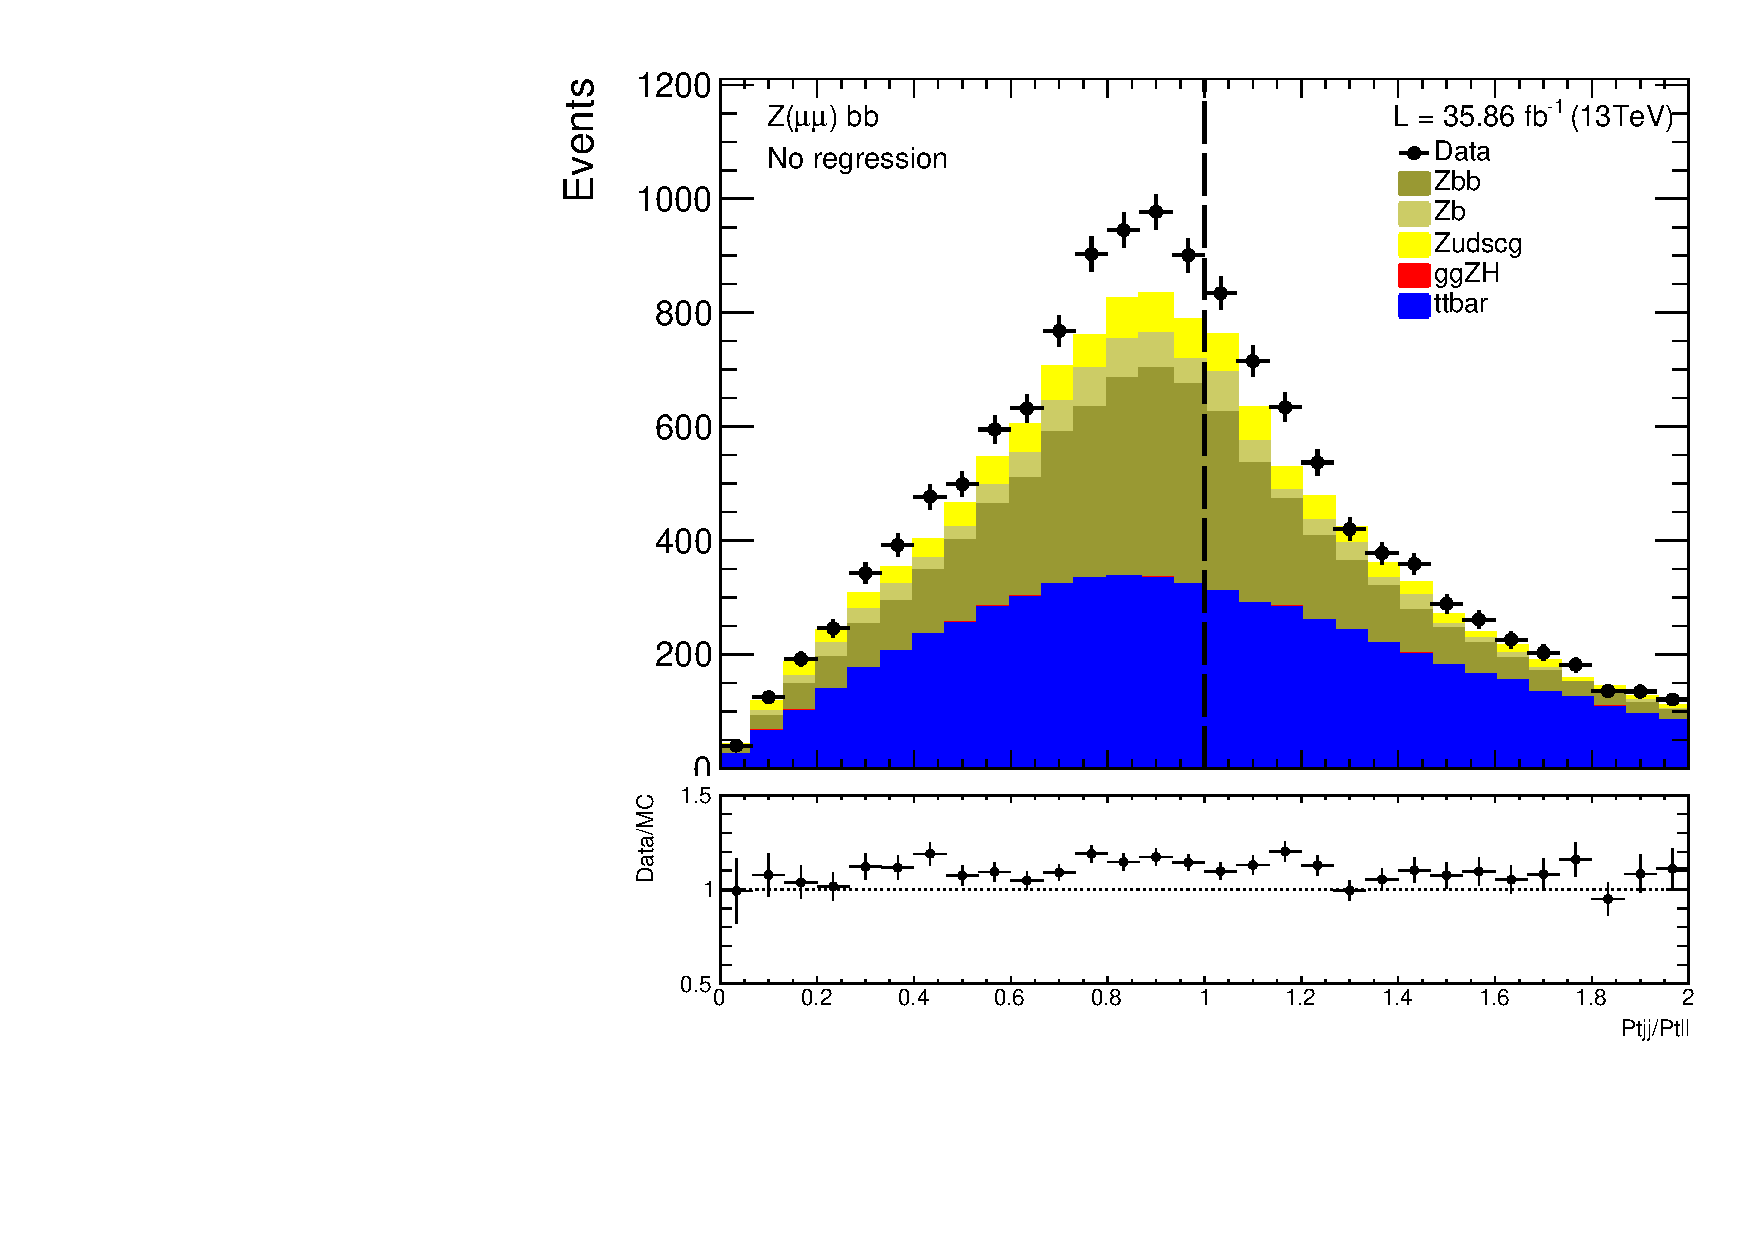
\includegraphics[width=0.32\textwidth]{b-reg/Vali_Data_MC_no_reg__PtBalance_mu_Medium}\hfil
  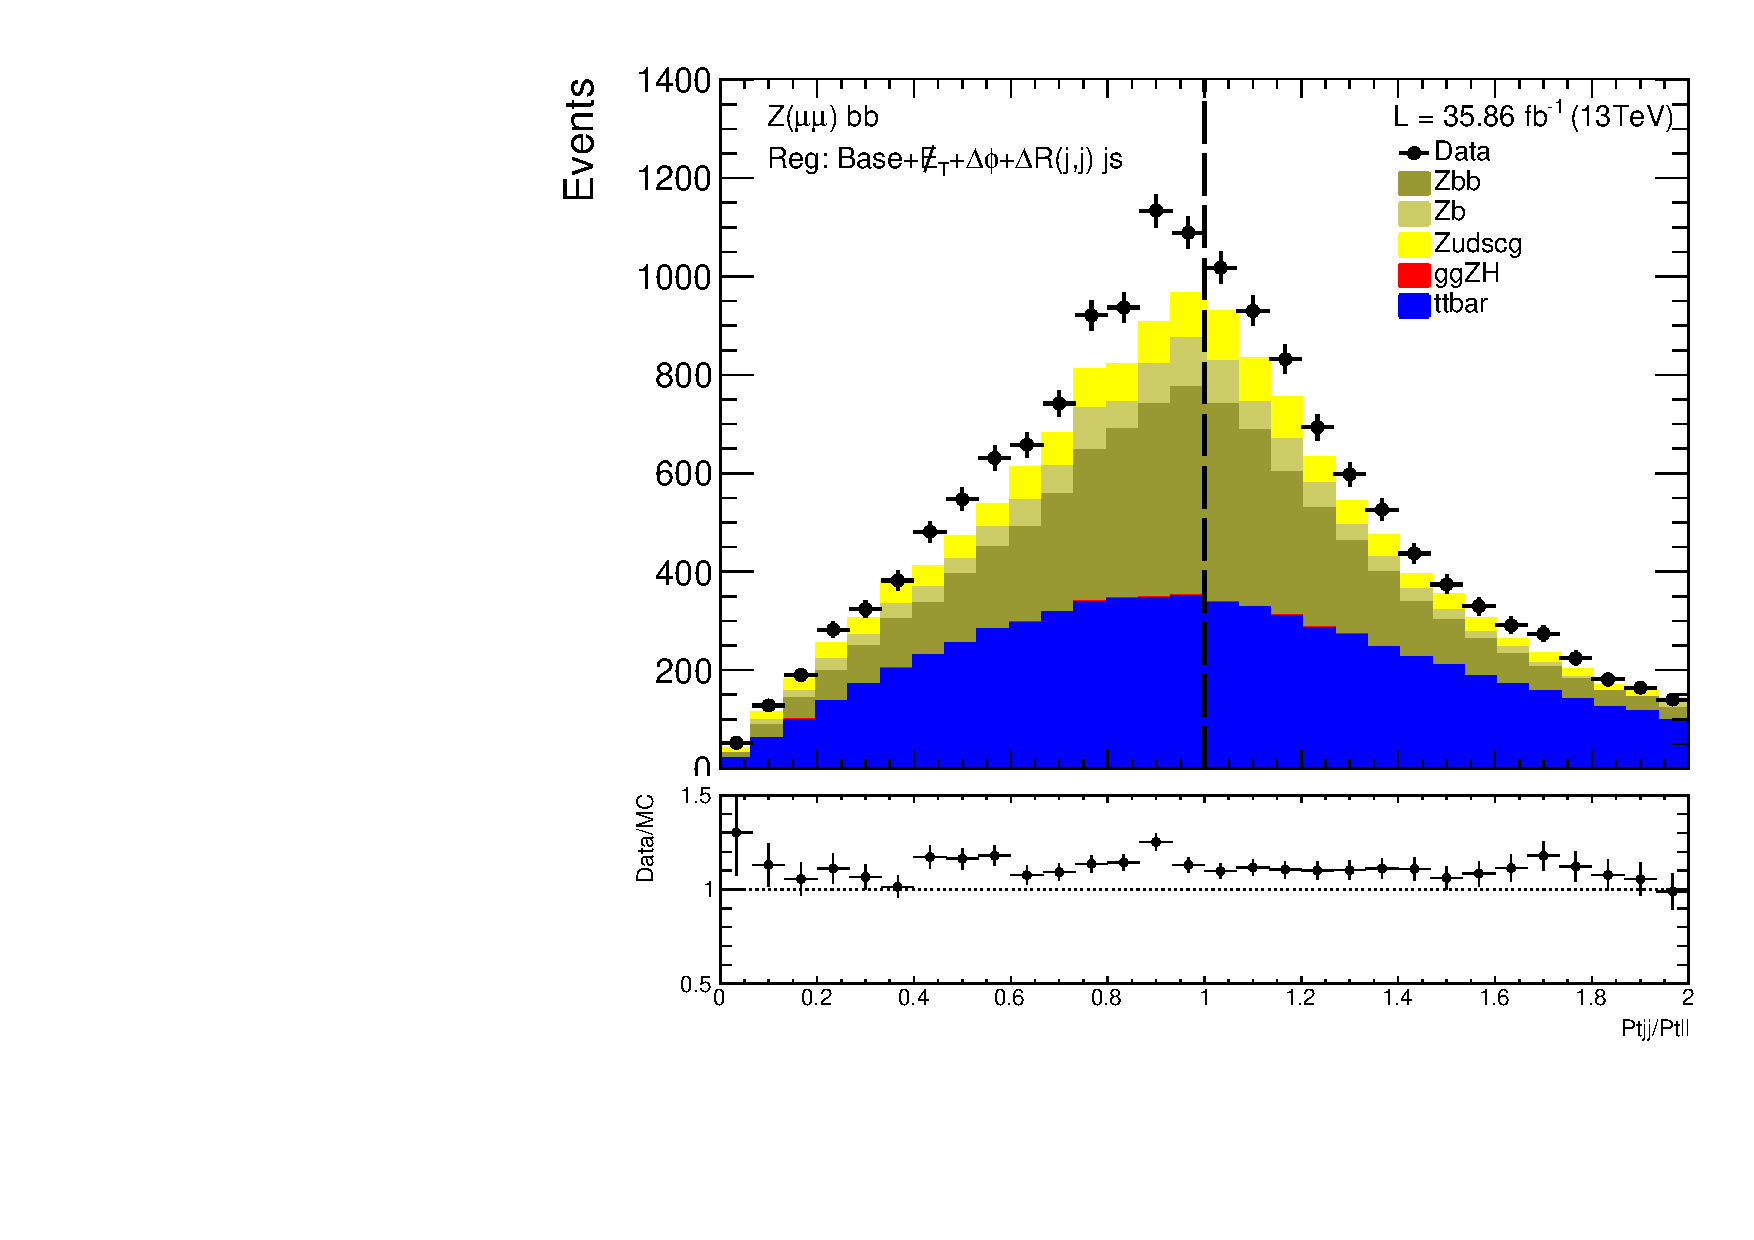
\includegraphics[width=0.32\textwidth]{b-reg/Vali_Data_MC_jet_15plus3_js_2_27__PtBalance_mu_Medium}\hfil
  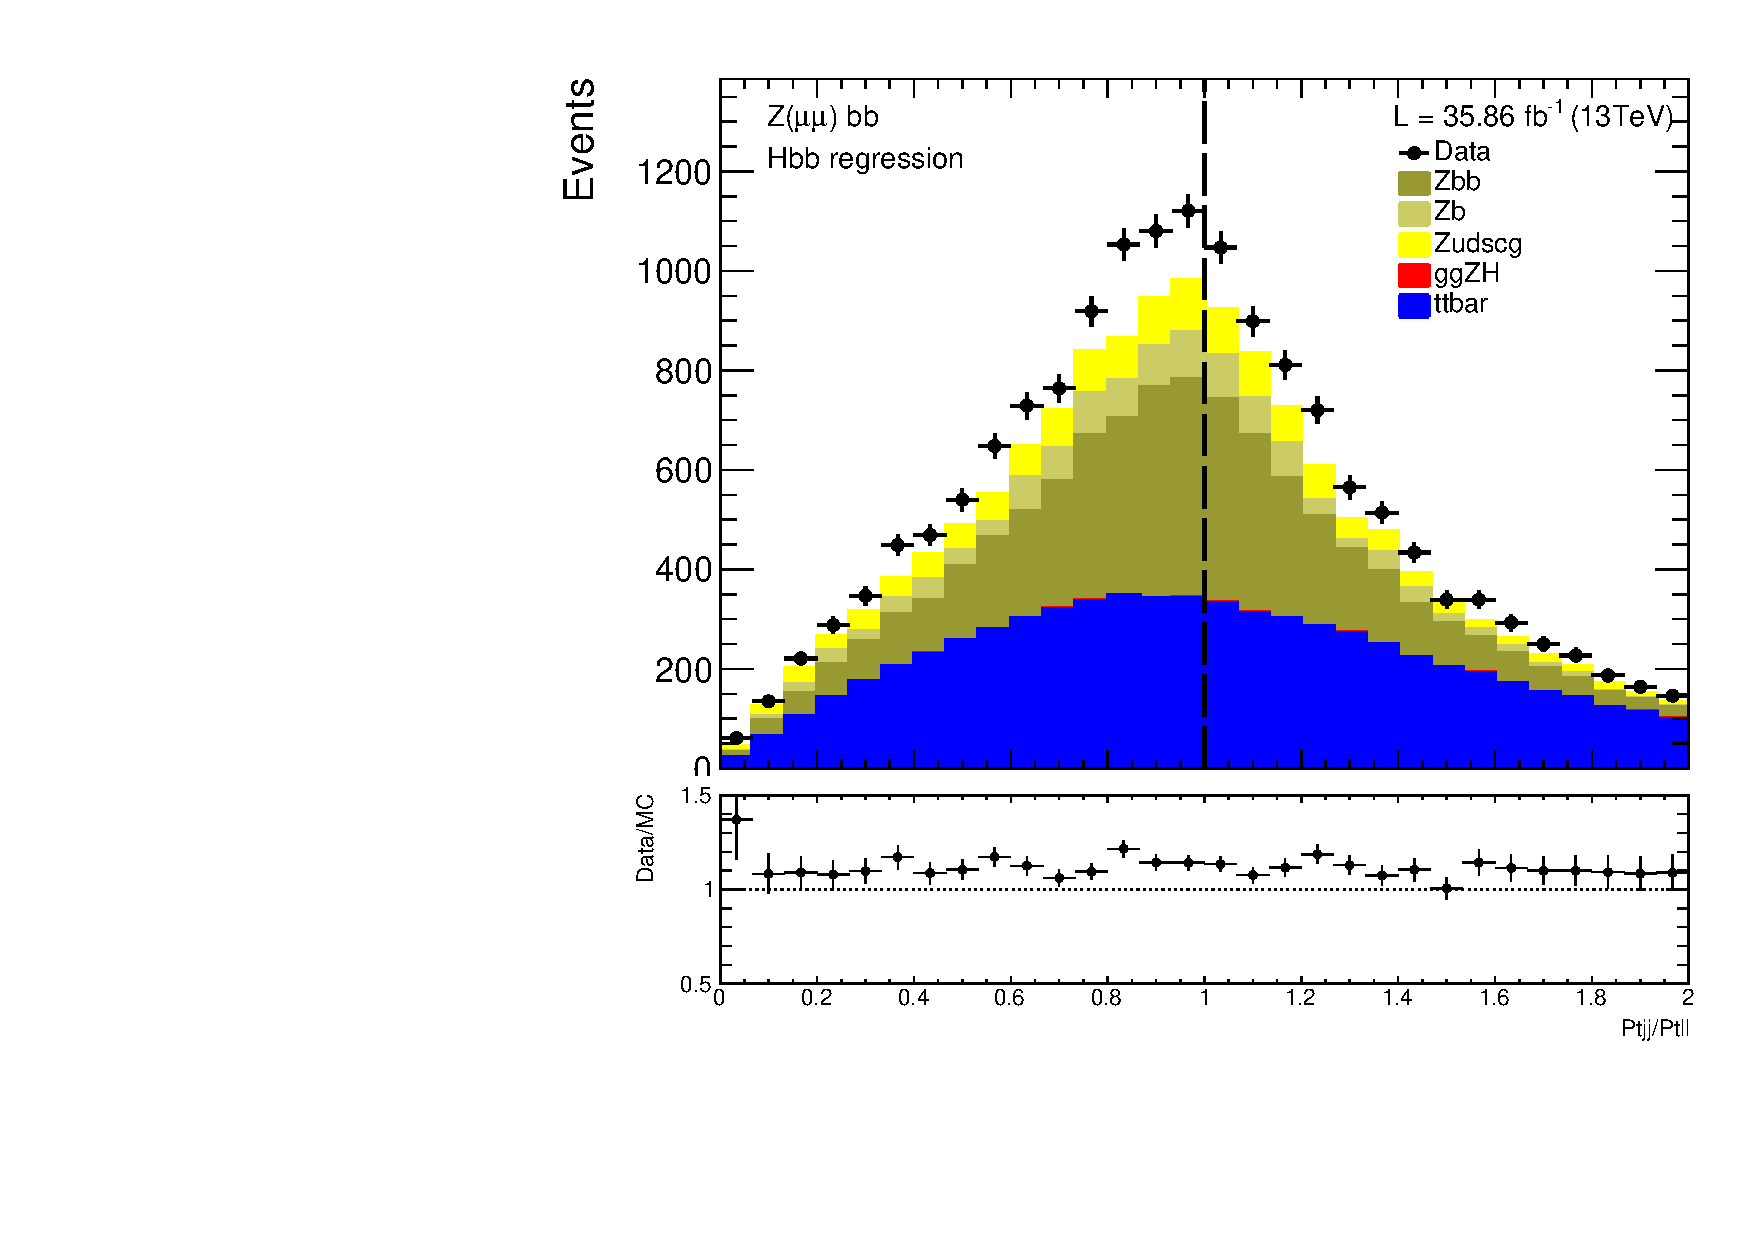
\includegraphics[width=0.32\textwidth]{b-reg/Vali_Data_MC_jet_Hbb__PtBalance_mu_Medium}\hfil\\
  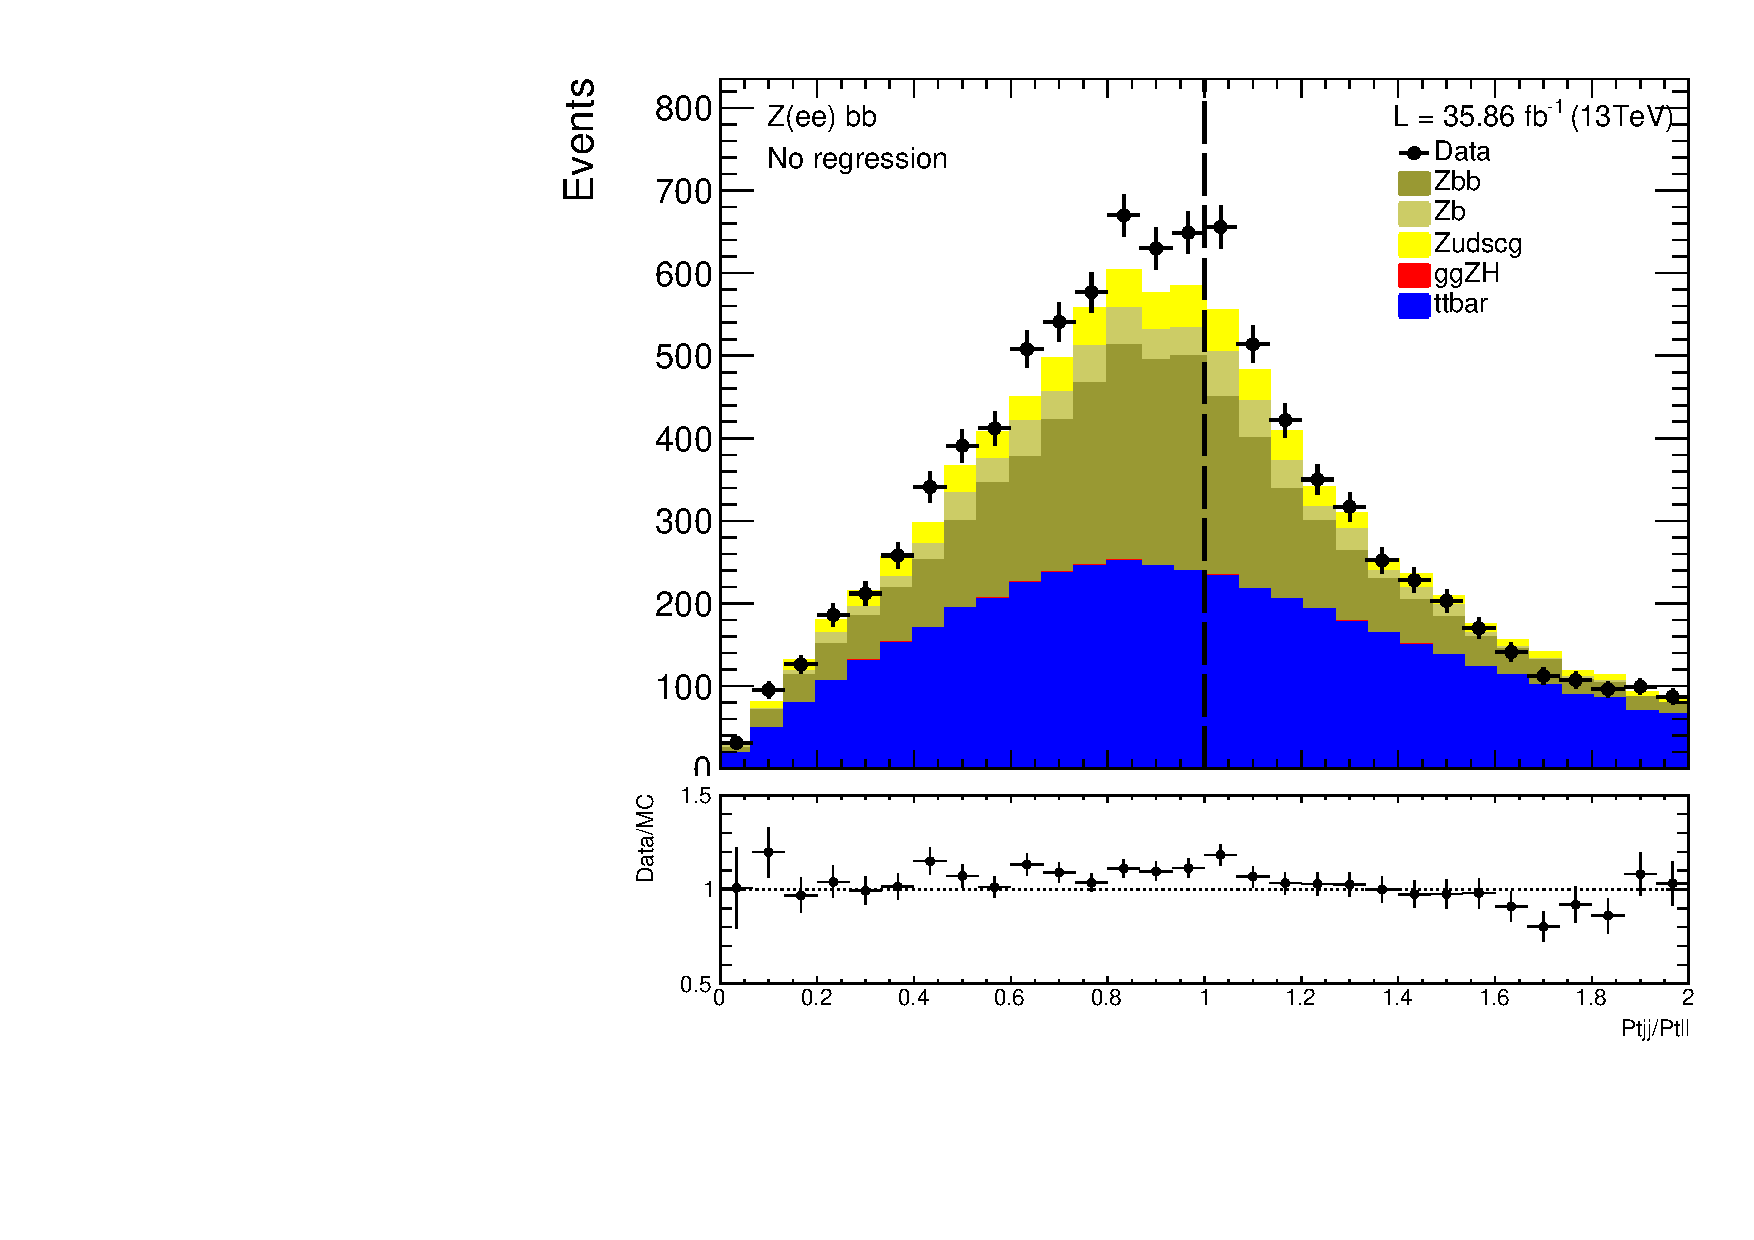
\includegraphics[width=0.32\textwidth]{b-reg/Vali_Data_MC_no_reg__PtBalance_ele_Medium}\hfil
  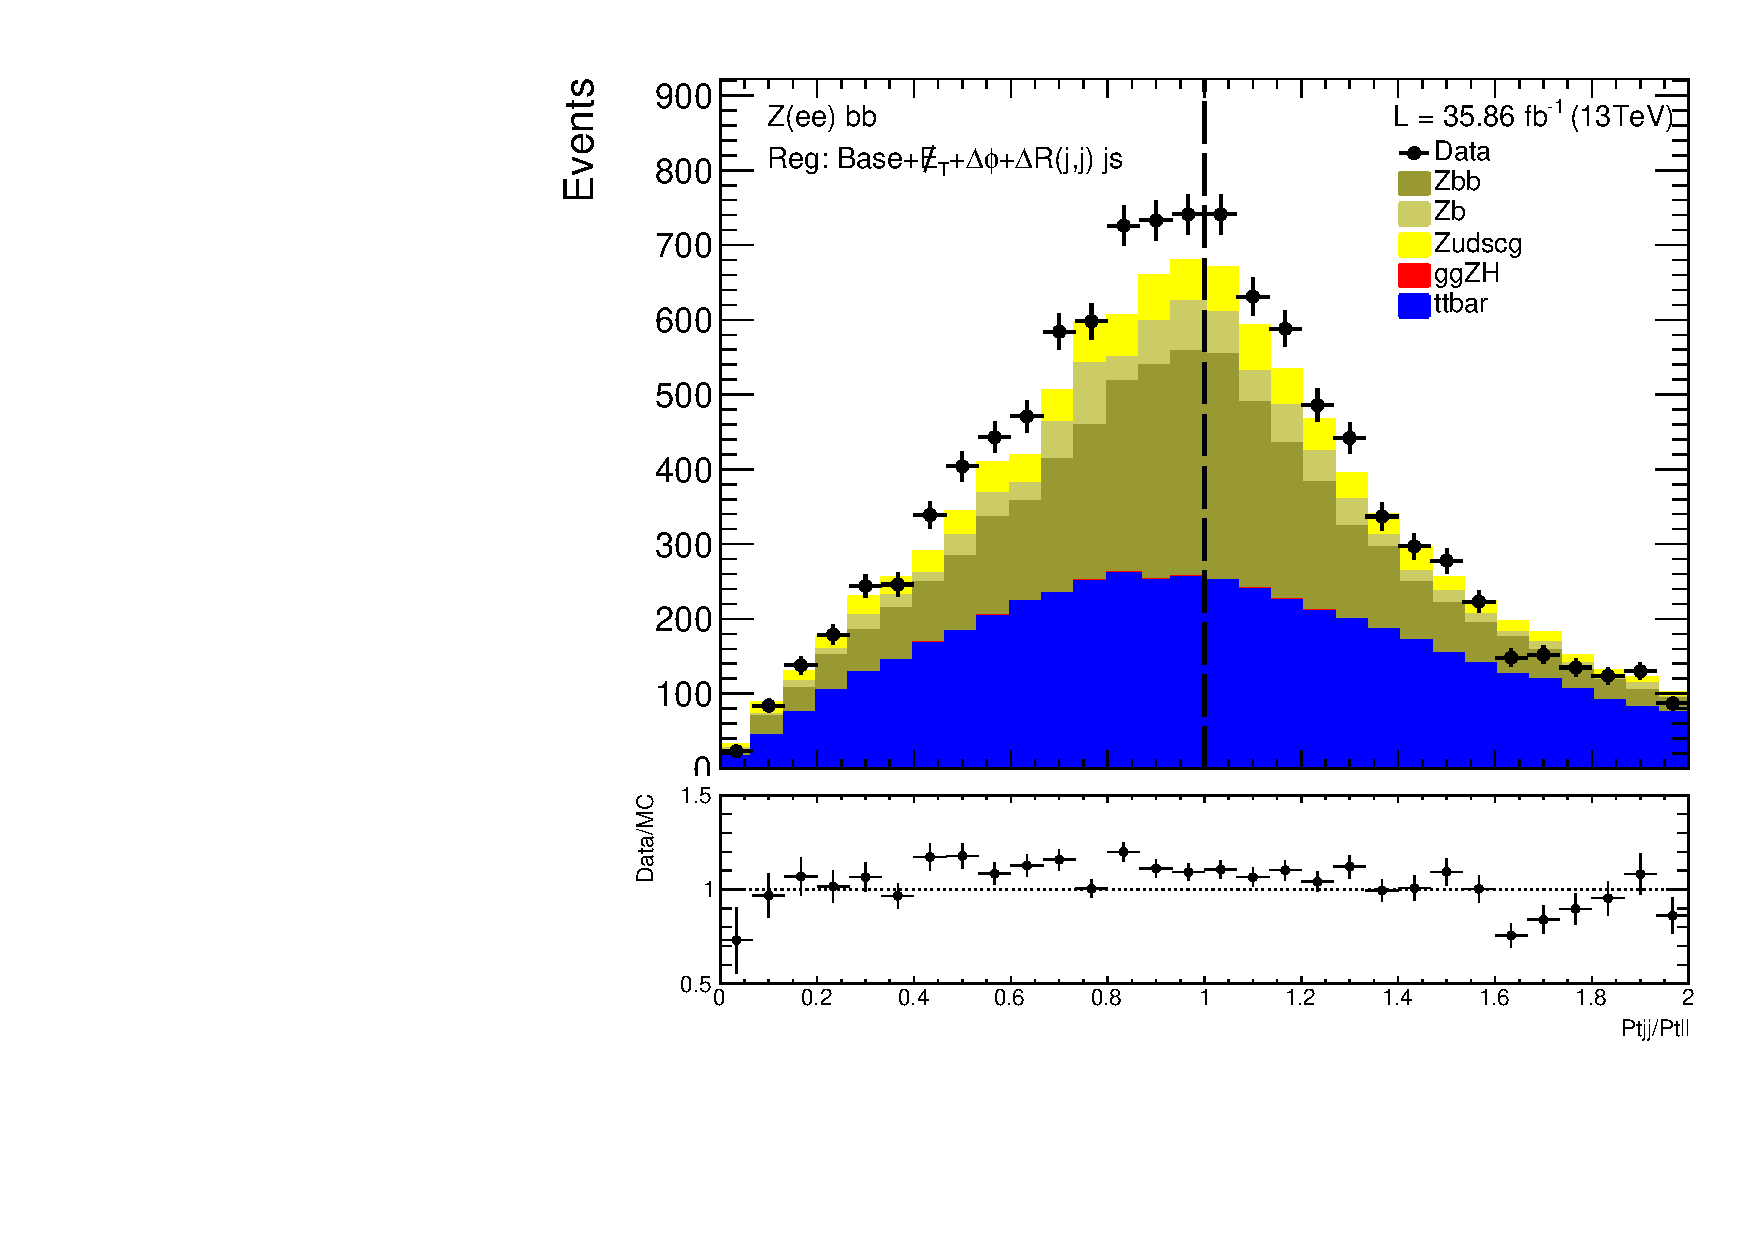
\includegraphics[width=0.32\textwidth]{b-reg/Vali_Data_MC_jet_15plus3_js_2_27__PtBalance_ele_Medium}\hfil
  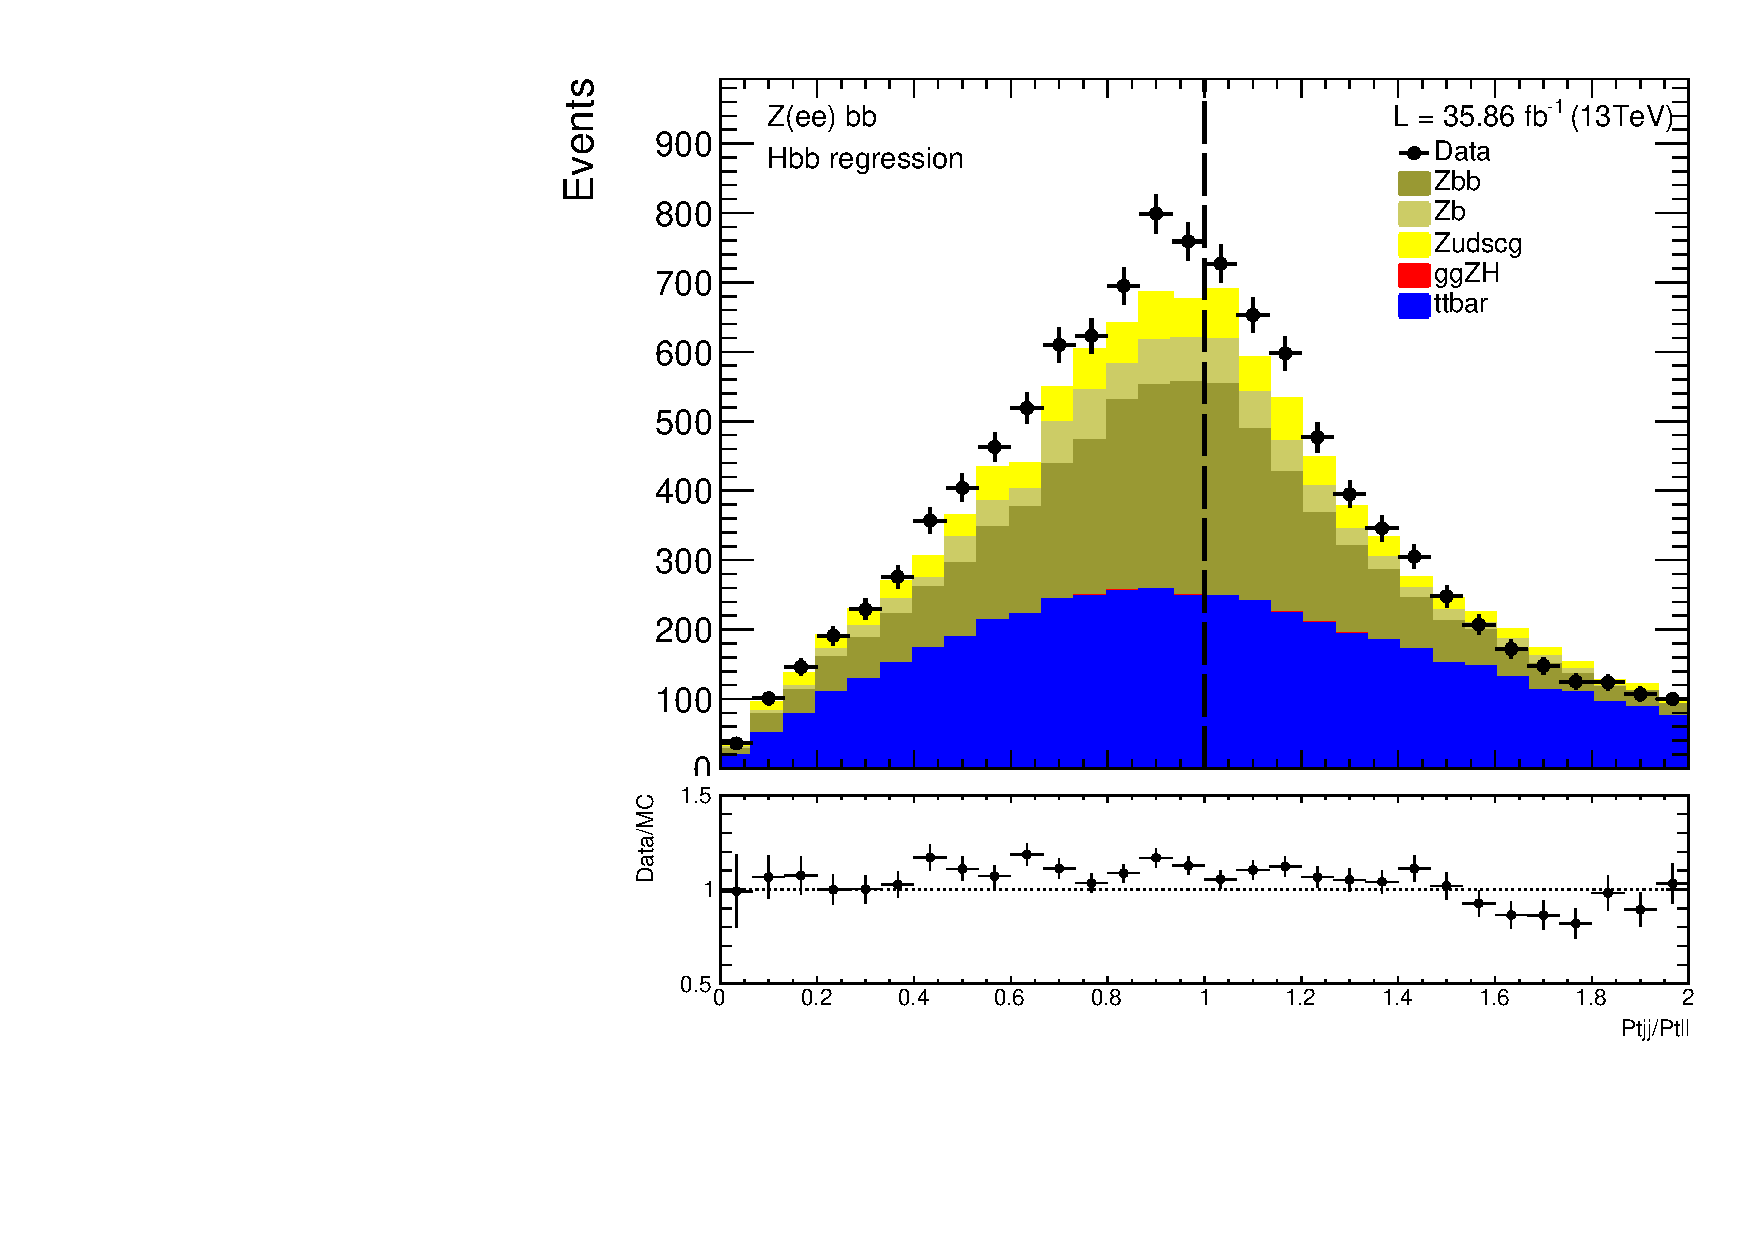
\includegraphics[width=0.32\textwidth]{b-reg/Vali_Data_MC_jet_Hbb__PtBalance_ele_Medium}\hfil\\
  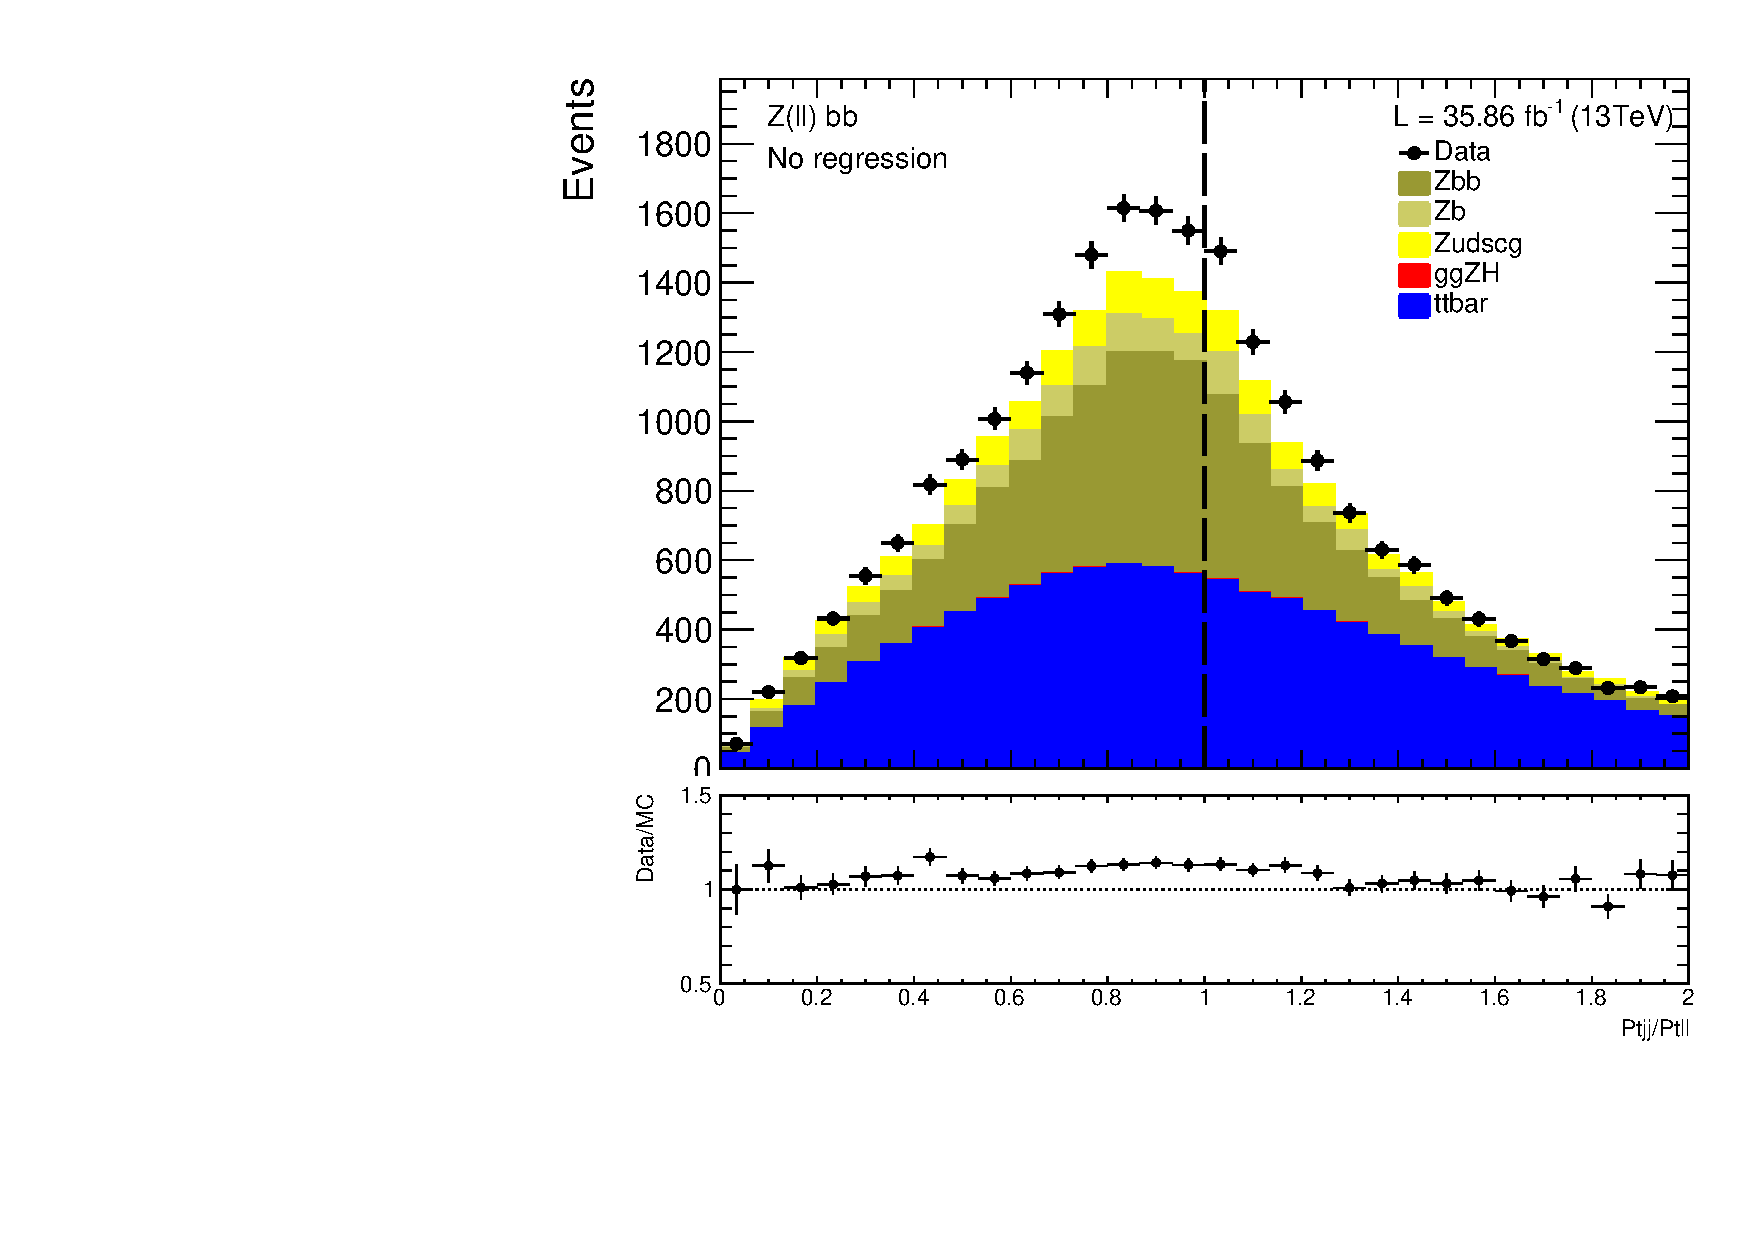
\includegraphics[width=0.32\textwidth]{b-reg/Vali_Data_MC_no_reg__PtBalance_all_Medium}\hfil
  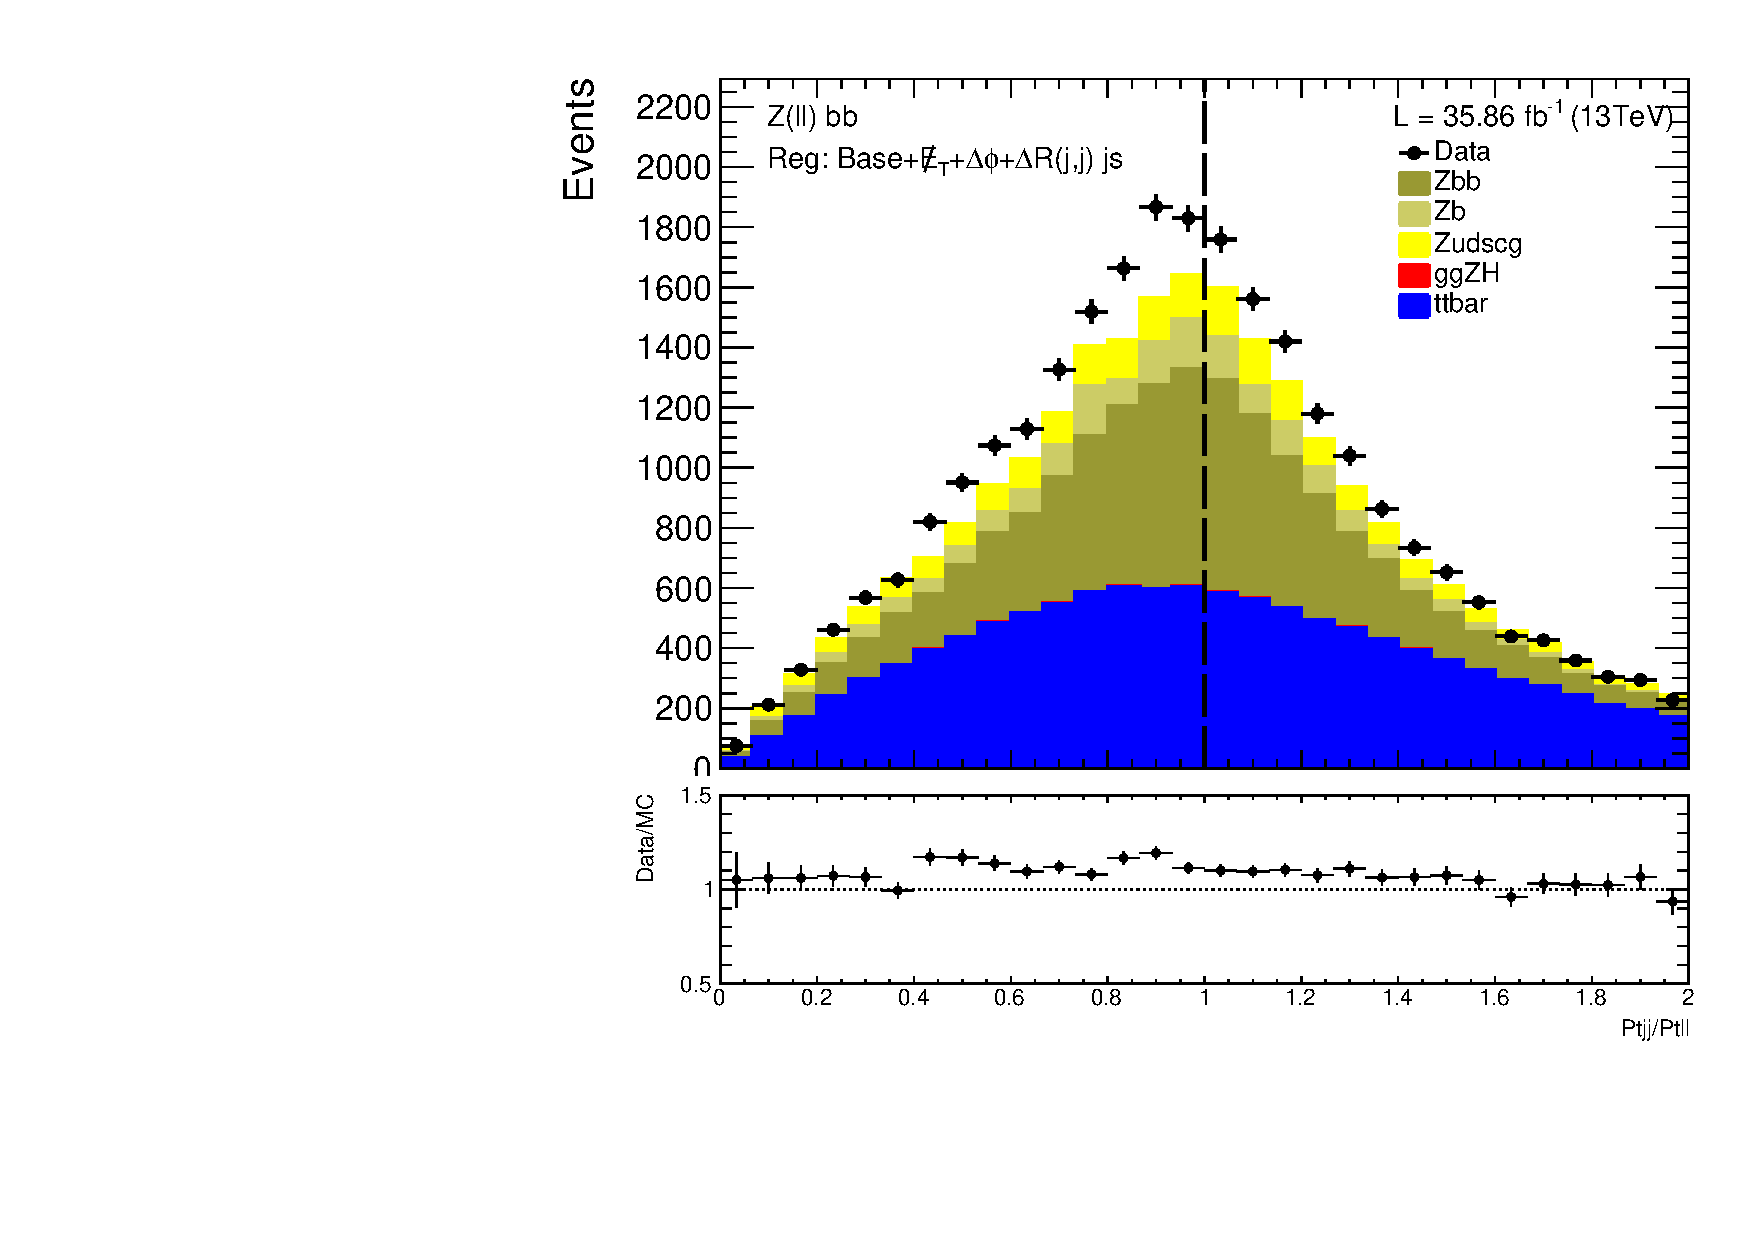
\includegraphics[width=0.32\textwidth]{b-reg/Vali_Data_MC_jet_15plus3_js_2_27__PtBalance_all_Medium}\hfil
  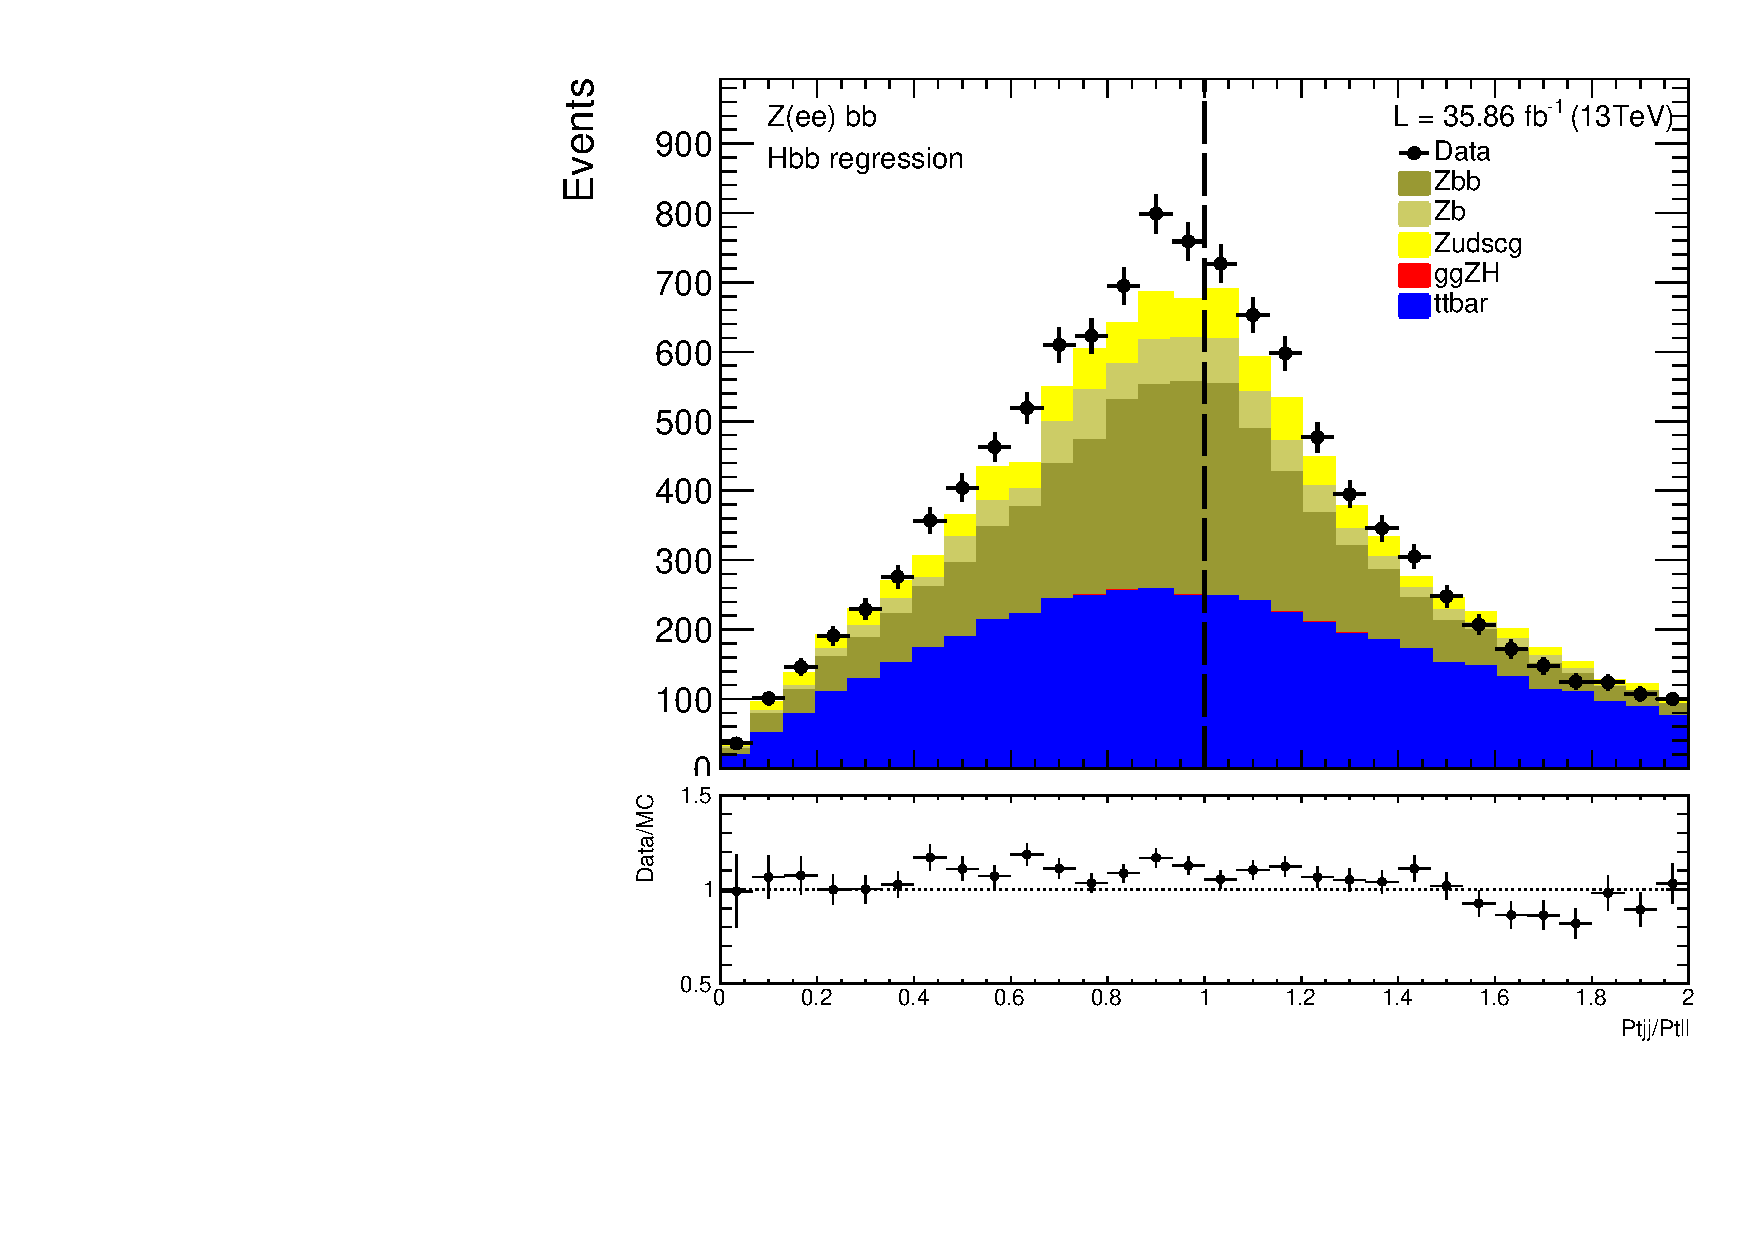
\includegraphics[width=0.32\textwidth]{b-reg/Vali_Data_MC_jet_Hbb__PtBalance_ele_Medium}\hfil\\
  \caption{Pt balance (ratio) of the di-jet and di-lepton. On the left
    are the distributions without regression, in the center - using
    \textbf{full 15+3var js} training and on the right - using
    \textbf{Hbb} regression.  Top plots are for muon channel, middle
    for electron channel and bottom is the combination (sum) of the
    two.}
  \label{fig:vali-pt}
\end{figure*}

Figure \ref{fig:vali-pt} shows the mentioned $\PT$-balance
distributions, $\PT^{jj}/\PT^{\ell\ell}$.  The data is compared to the
MC predictions. It can be seen that before any regression is applied to avoid over training.
(left plots) the peak of the ratio distribution is below one. With the
regression applied the peak moves to 1 for both our \textbf{full variables with js}
 training (center) and the one from \textbf{Hbb} (right). The
trend is the same in data and MC.  This indicates that the regression
does indeed brings the $\PT$ of the $b$-jets closer to their true
values.

Similarly, figure~\ref{fig:vali-Mjj} shows the mass distributions,
$m_{jj}$, before and after regression. These figures indicate that
$m_{jj}$ is not distorted in any bad way, no artificial peaks are
created. This ensures us that the background distributions in our
analysis signal region will not be distorted either.


\begin{figure*}[thb]
  \centering
  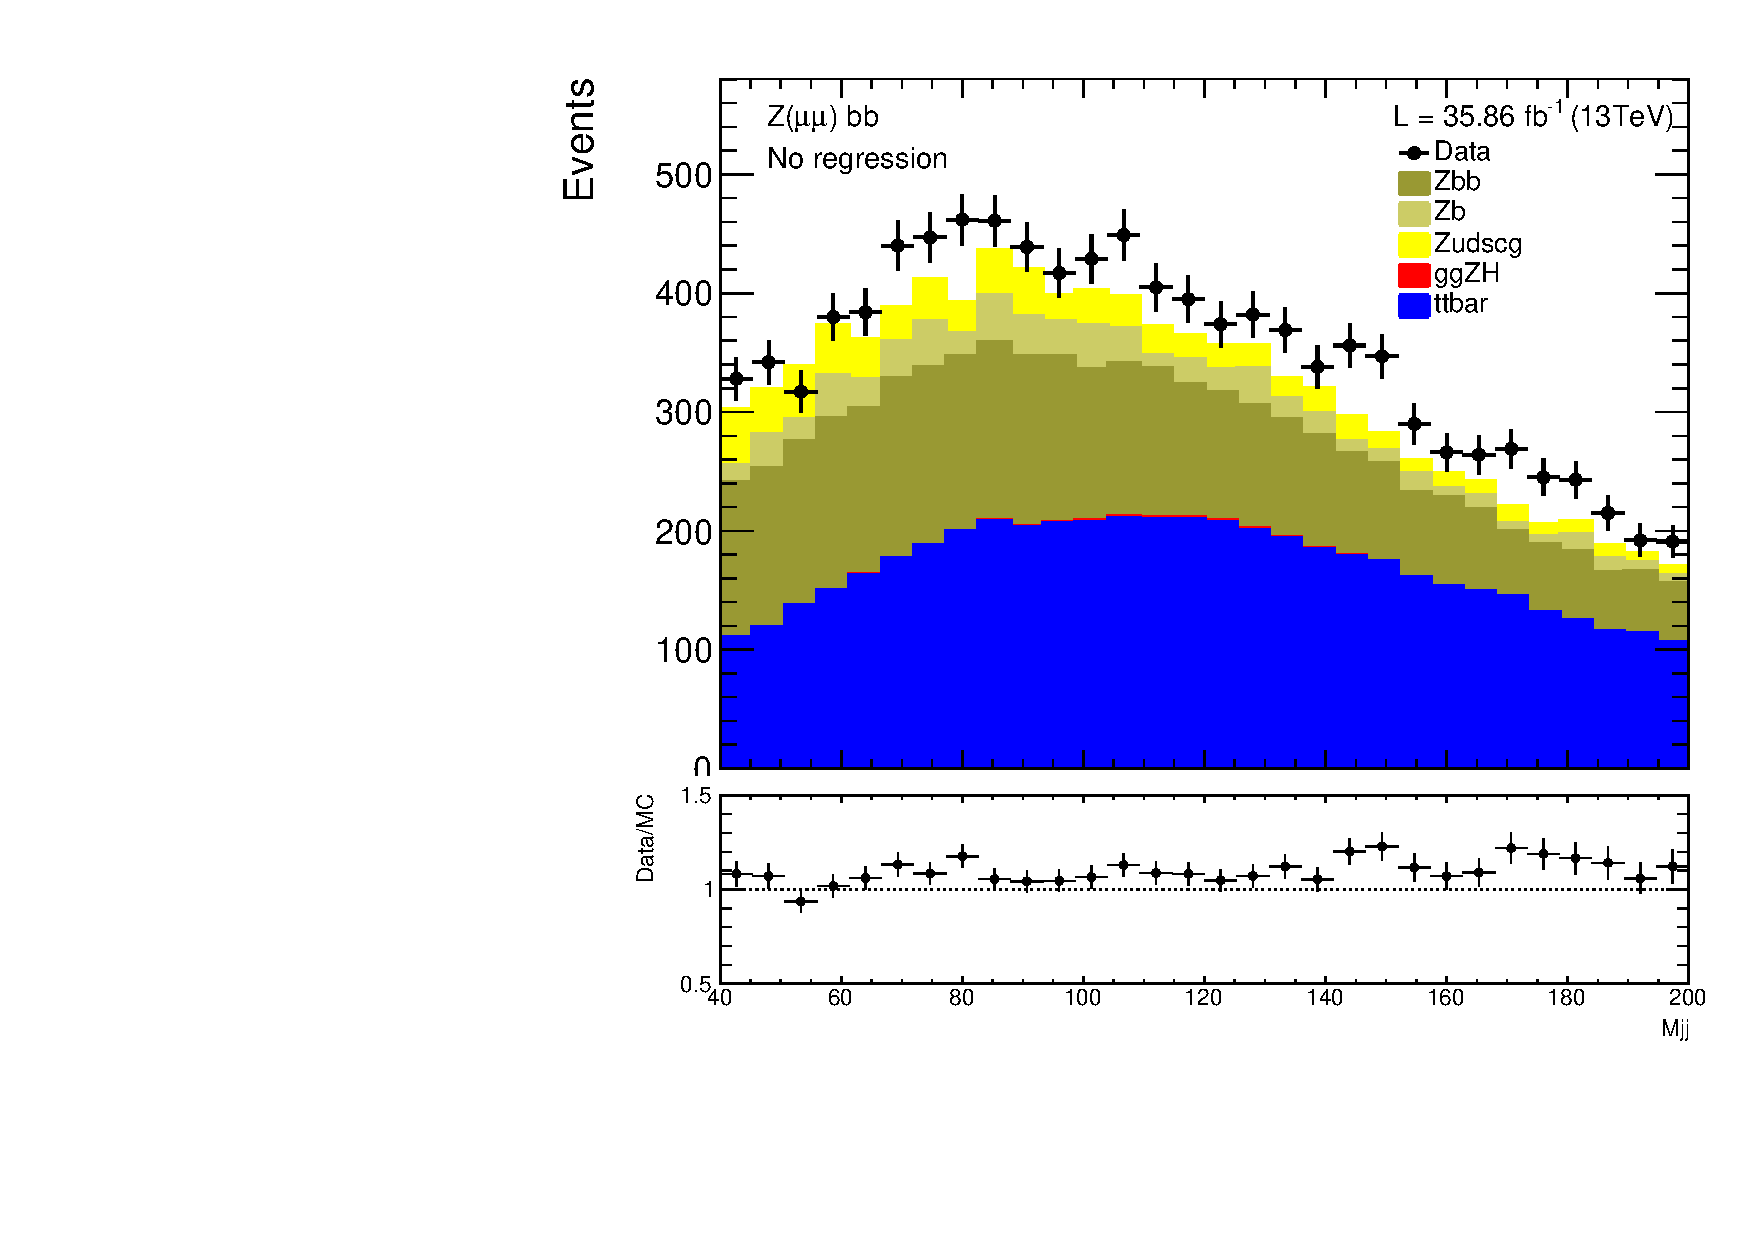
\includegraphics[width=0.32\textwidth]{b-reg/Vali_Data_MC_no_reg__Mjj_mu_Medium}\hfil
  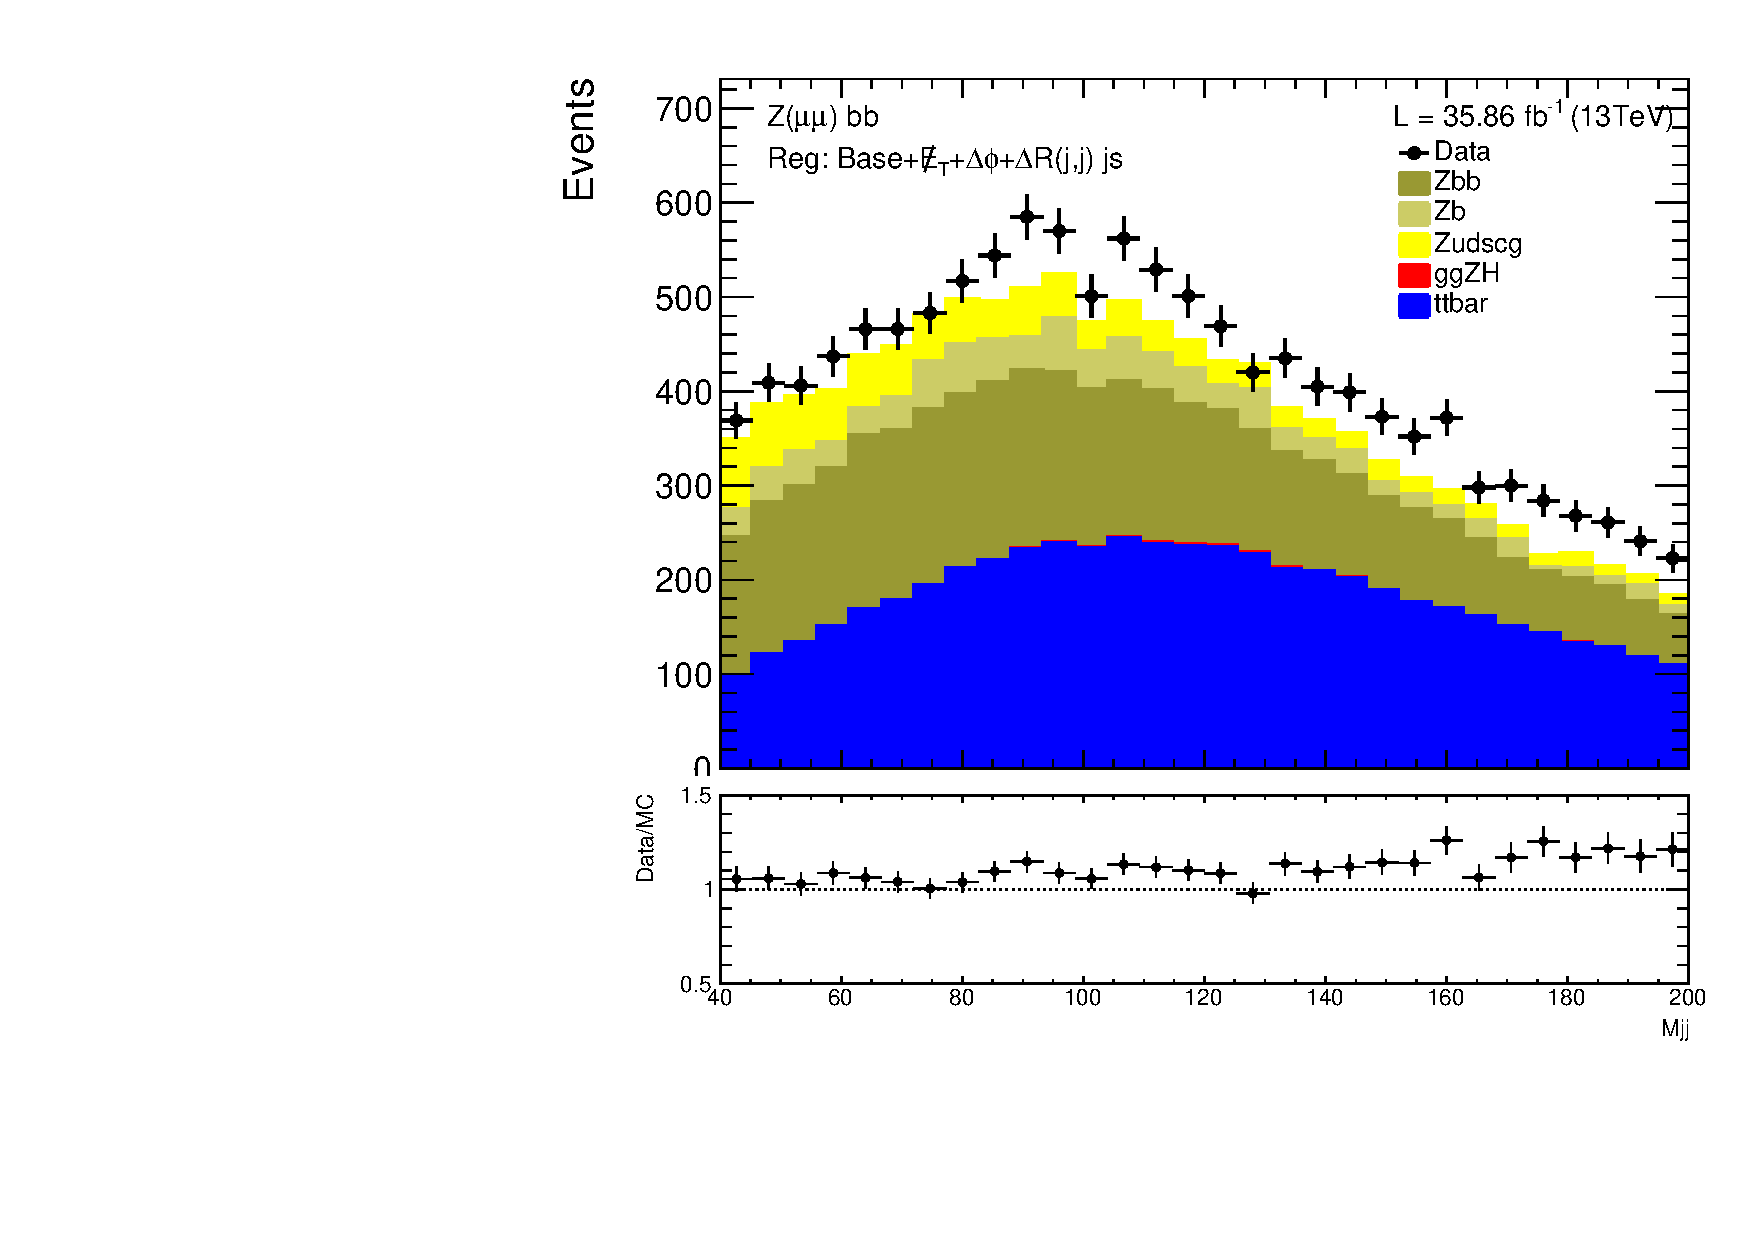
\includegraphics[width=0.32\textwidth]{b-reg/Vali_Data_MC_jet_15plus3_js_2_27__Mjj_mu_Medium}\hfil
  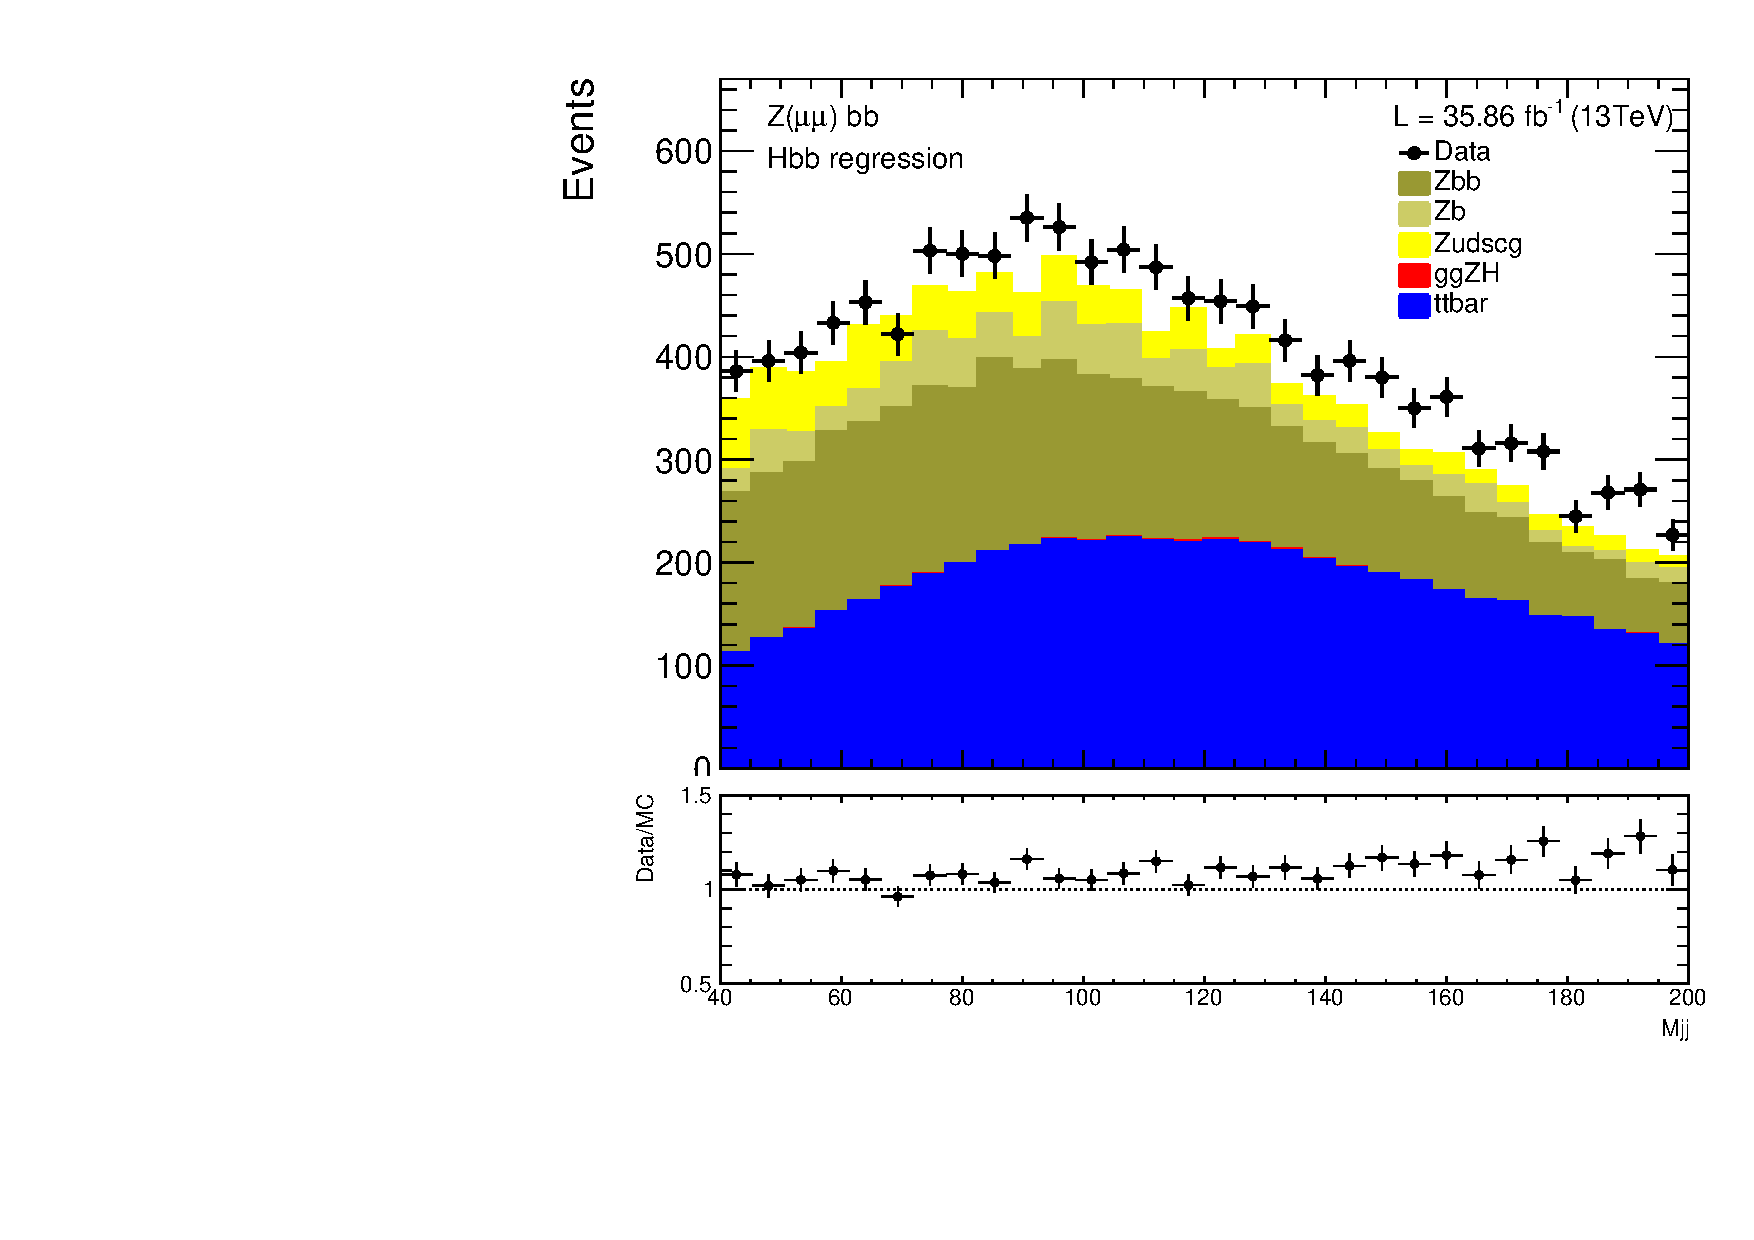
\includegraphics[width=0.32\textwidth]{b-reg/Vali_Data_MC_jet_Hbb__Mjj_mu_Medium}\hfil\\
  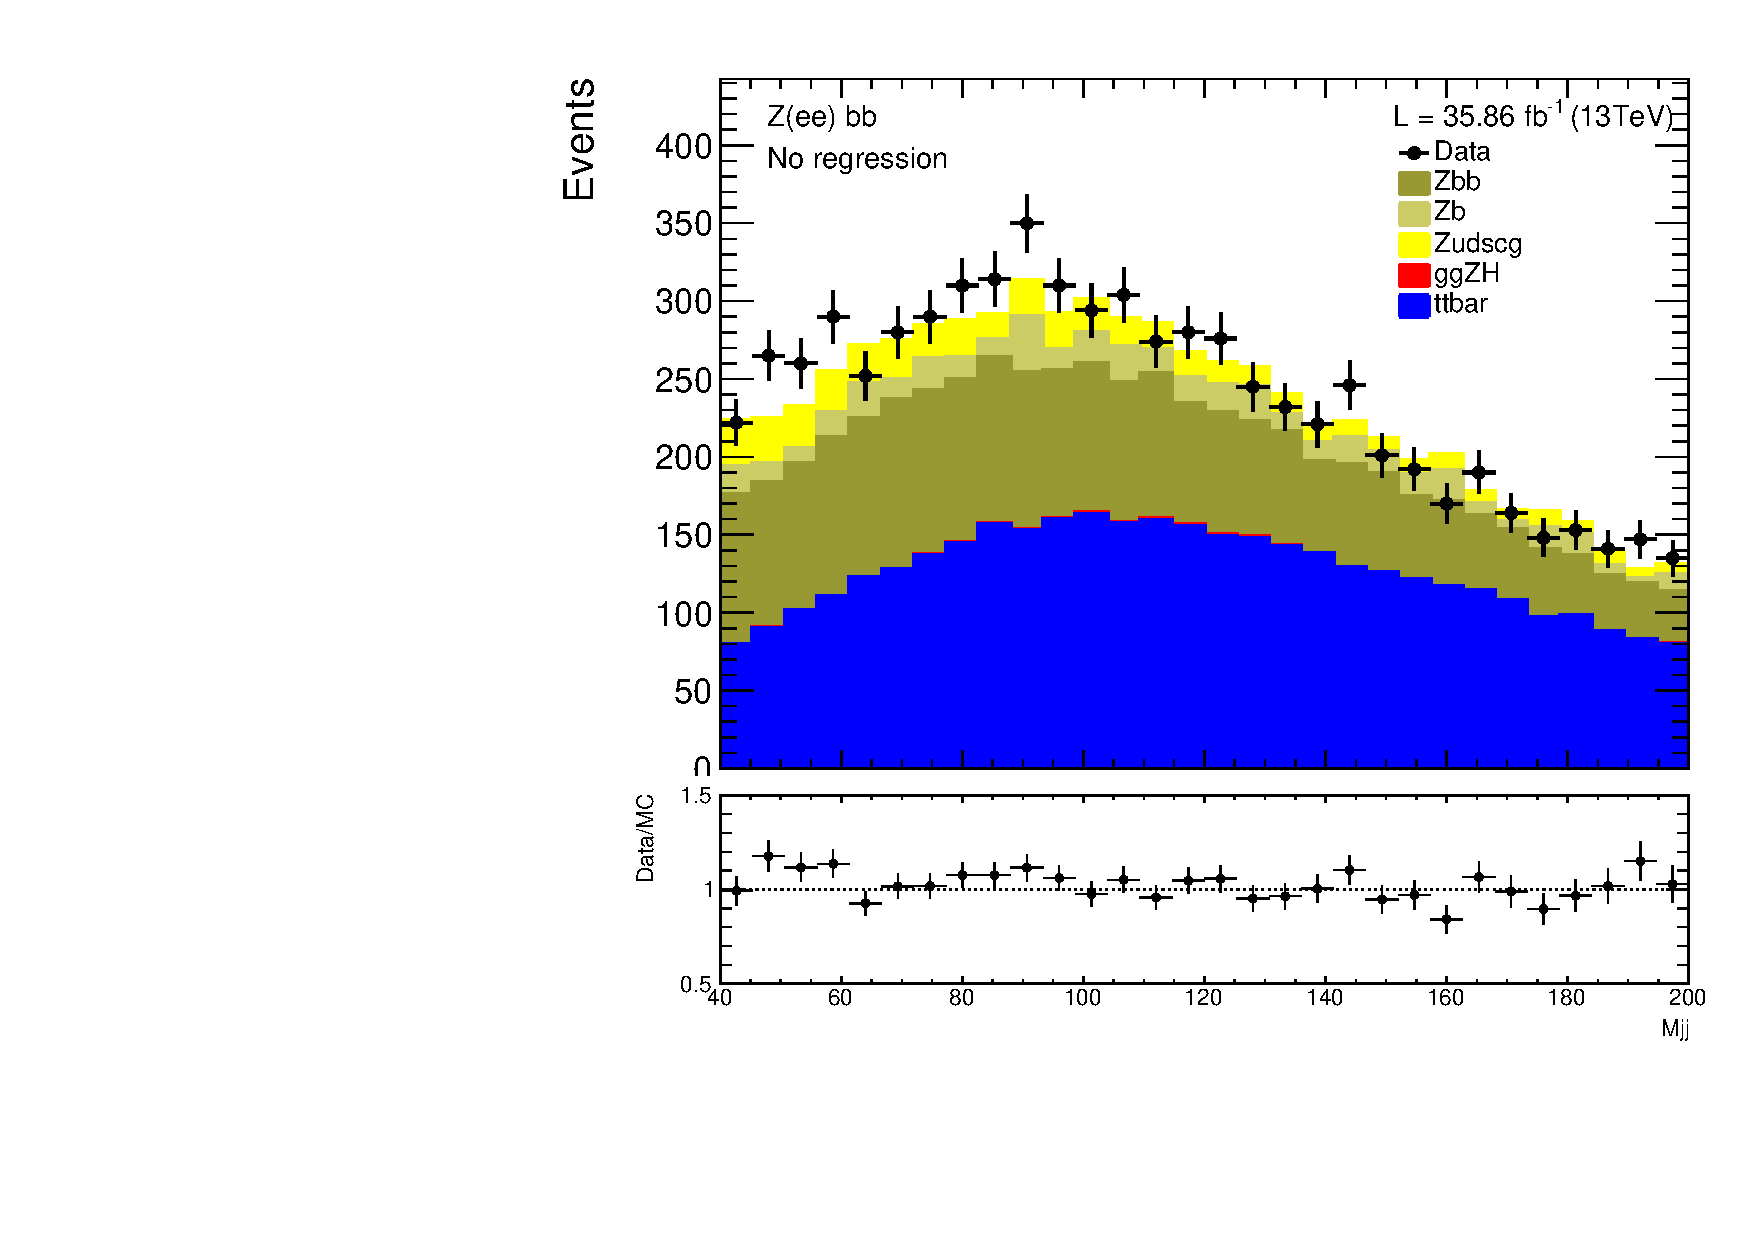
\includegraphics[width=0.32\textwidth]{b-reg/Vali_Data_MC_no_reg__Mjj_ele_Medium}\hfil
  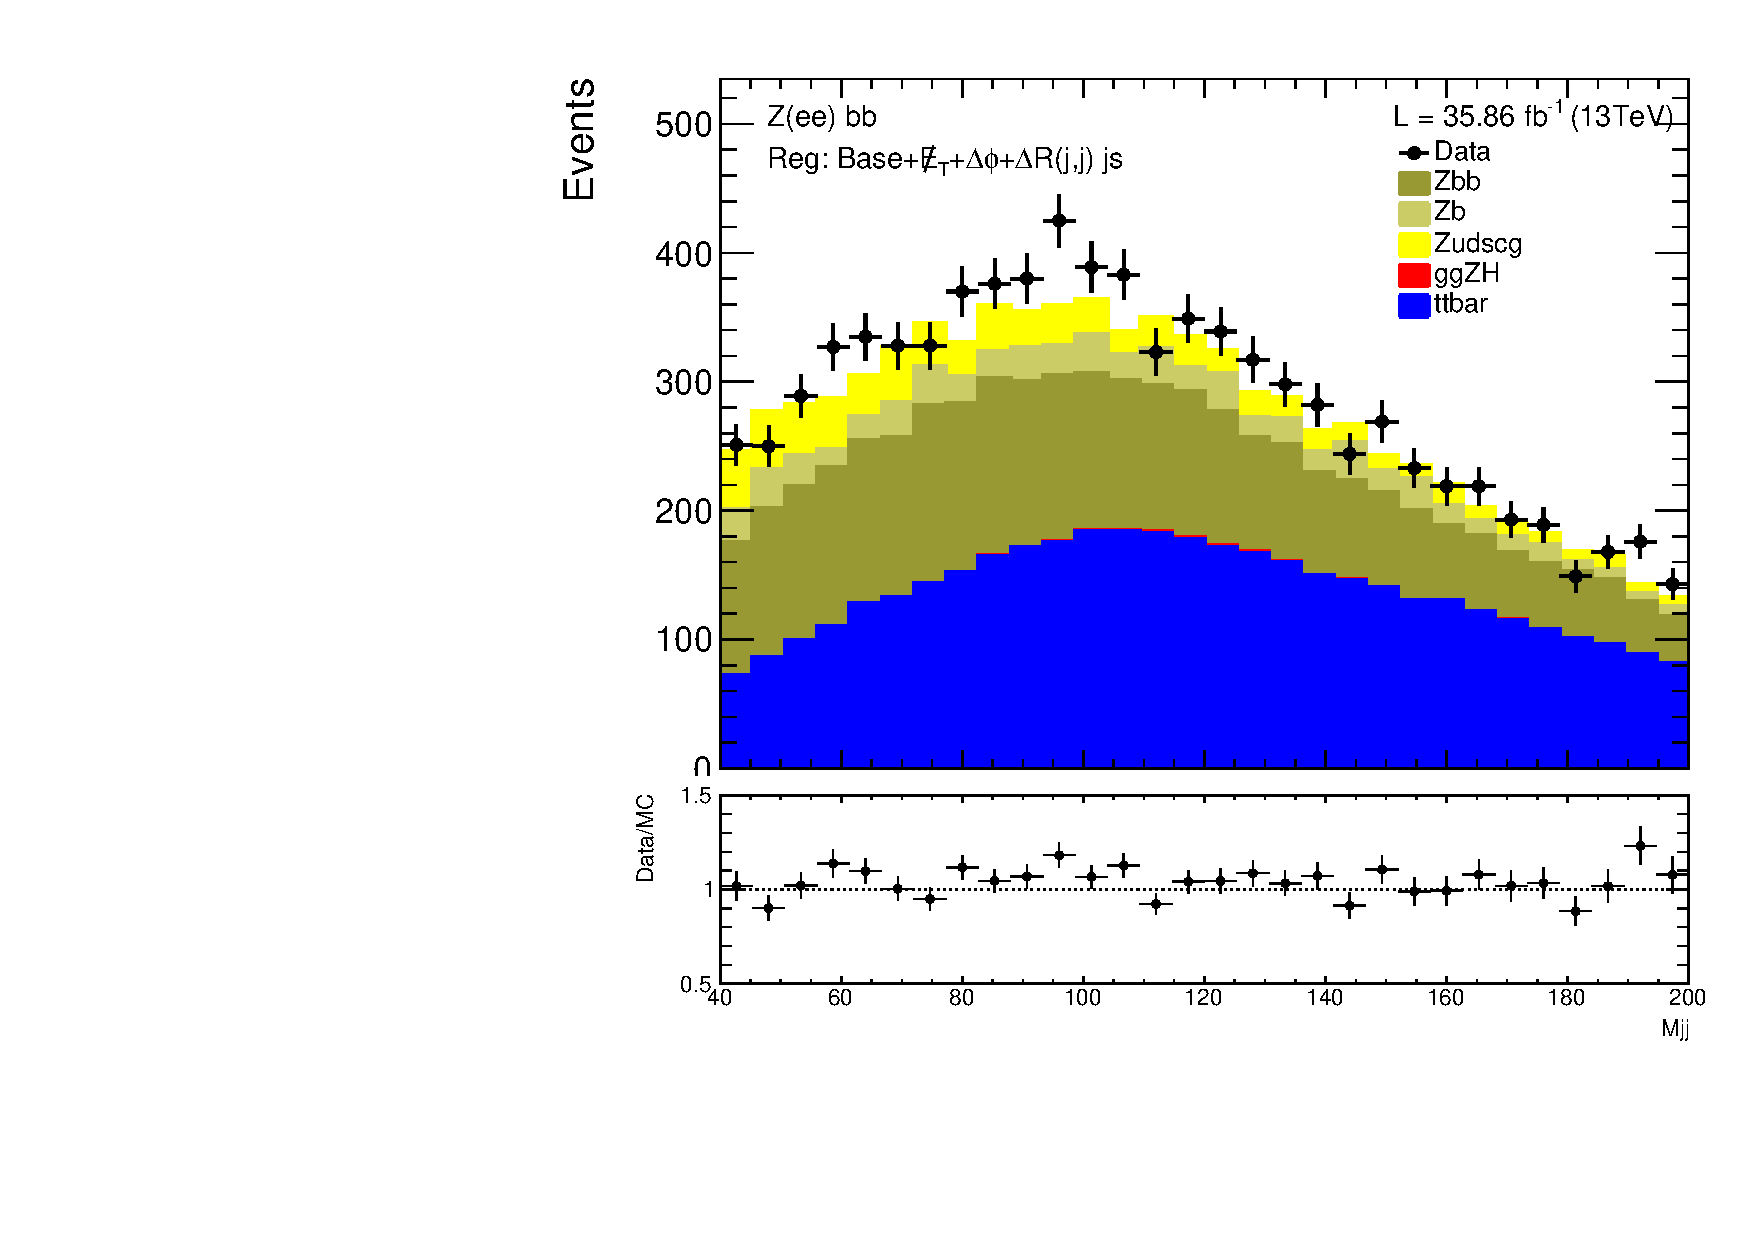
\includegraphics[width=0.32\textwidth]{b-reg/Vali_Data_MC_jet_15plus3_js_2_27__Mjj_ele_Medium}\hfil
  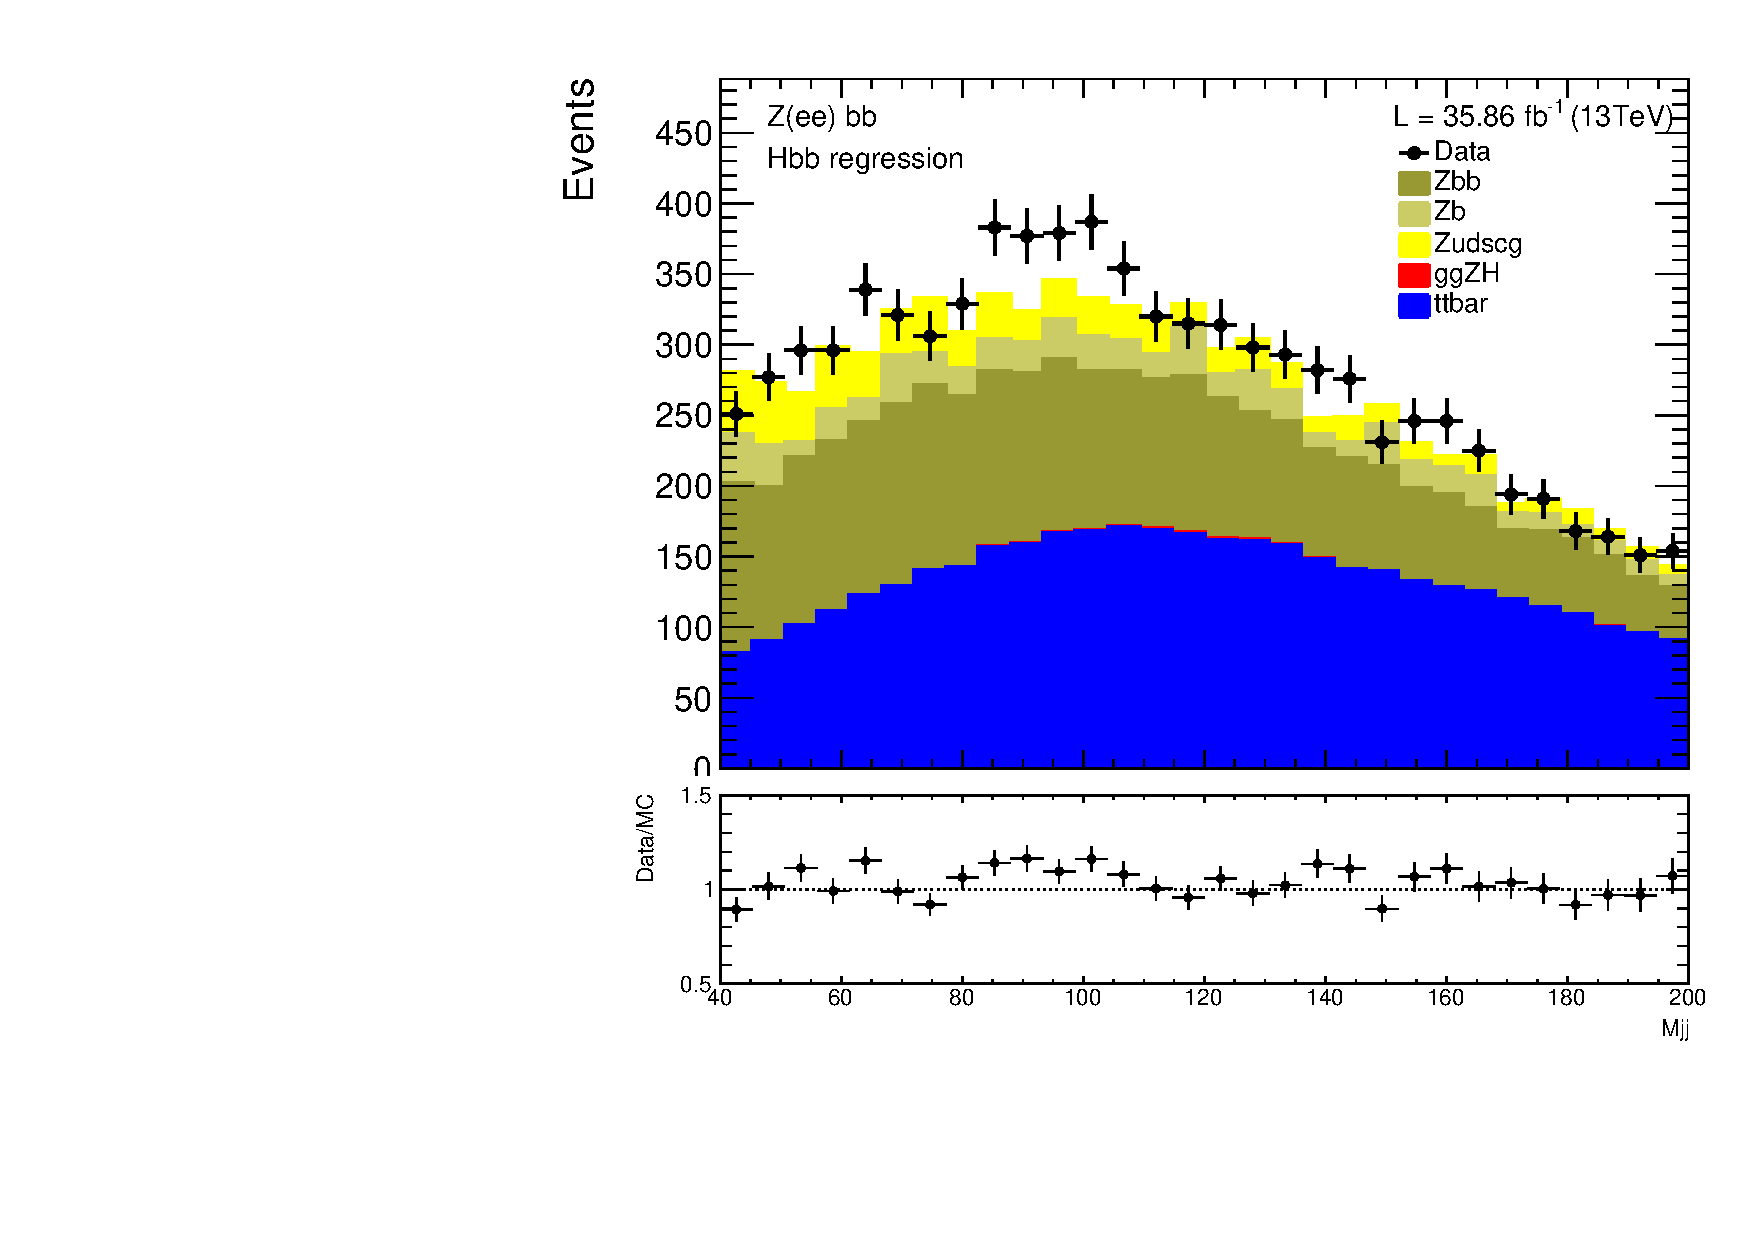
\includegraphics[width=0.32\textwidth]{b-reg/Vali_Data_MC_jet_Hbb__Mjj_ele_Medium}\hfil\\
  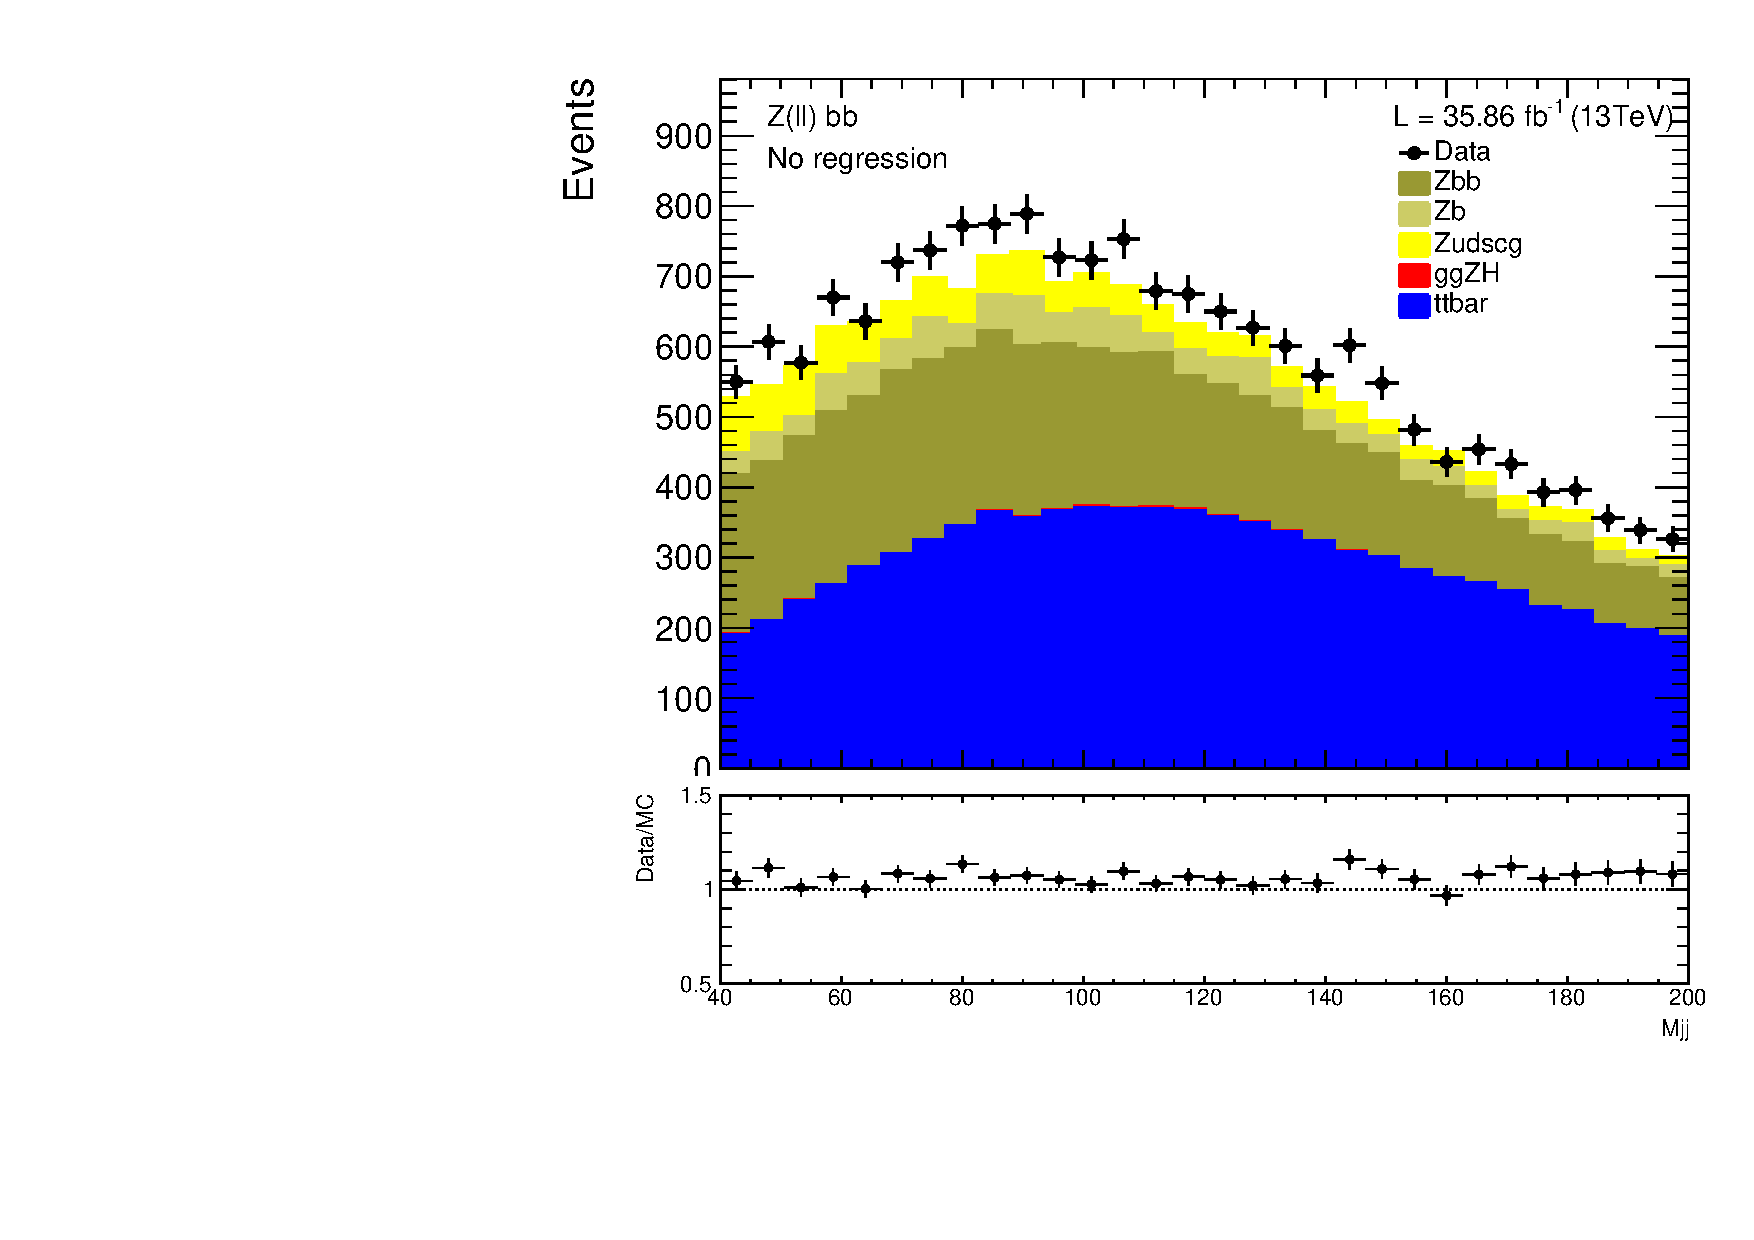
\includegraphics[width=0.32\textwidth]{b-reg/Vali_Data_MC_no_reg__Mjj_all_Medium}\hfil
  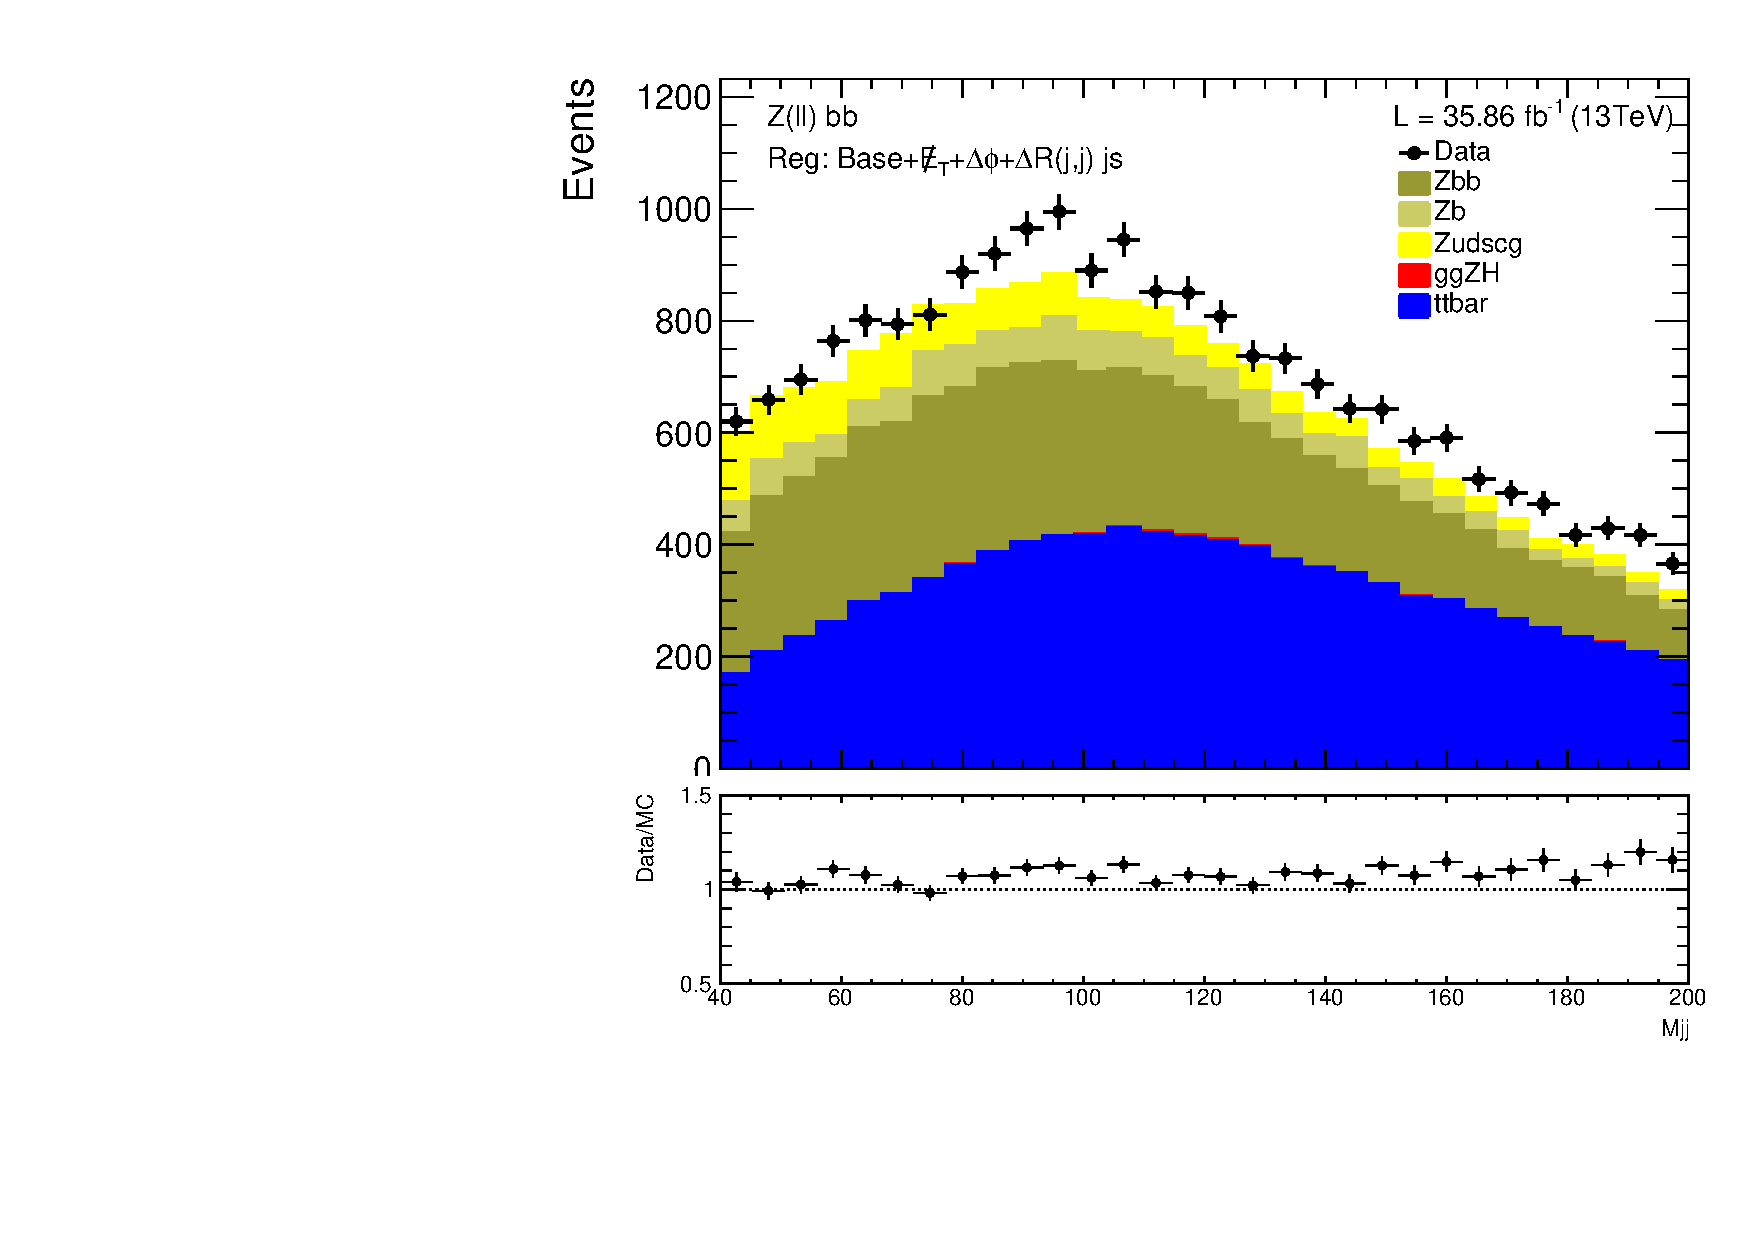
\includegraphics[width=0.32\textwidth]{b-reg/Vali_Data_MC_jet_15plus3_js_2_27__Mjj_all_Medium}\hfil
  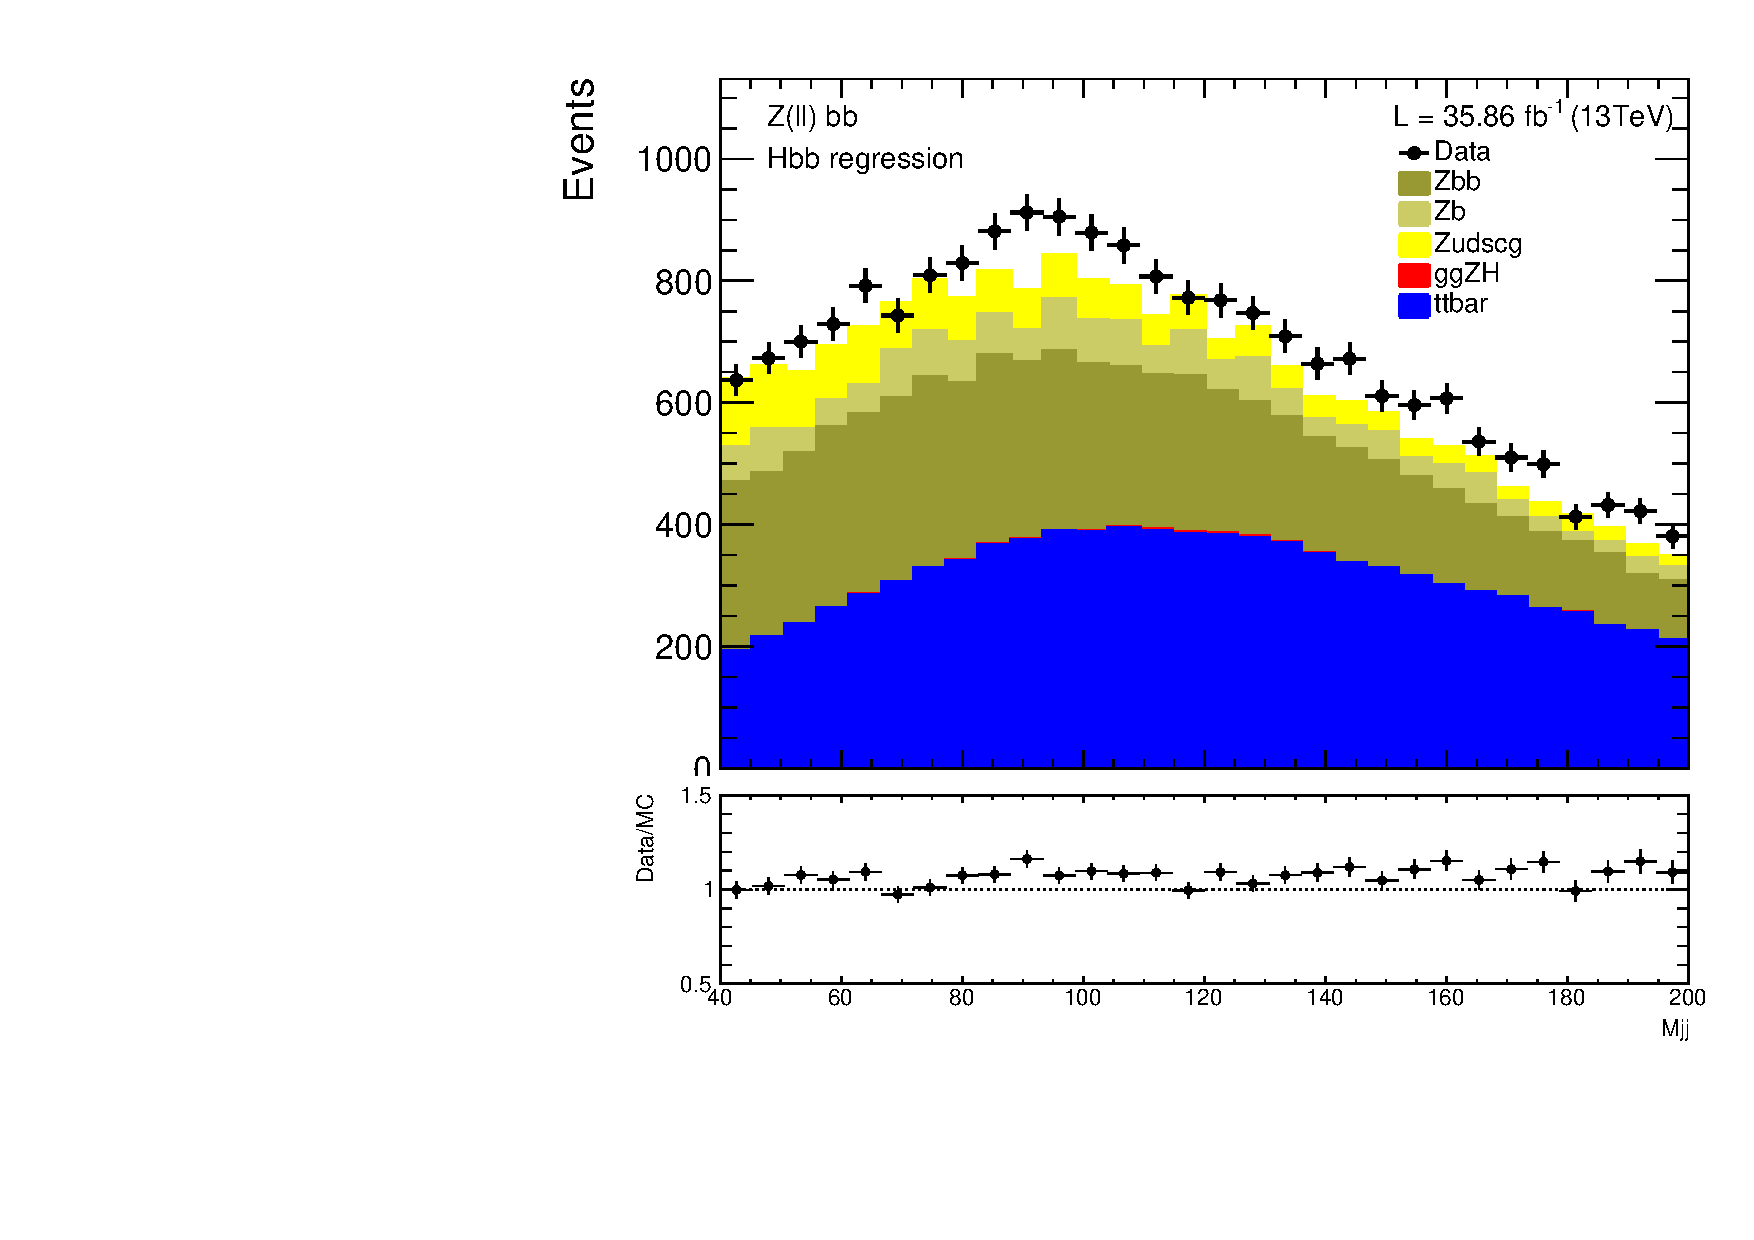
\includegraphics[width=0.32\textwidth]{b-reg/Vali_Data_MC_jet_Hbb__Mjj_all_Medium}\hfil\\
  \caption{Distributions of the $m_{jj}$. On the left are plots with
    no regression, in the center - using \textbf{full 15+3var js}
    training and on the right - using \textbf{Hbb} regression.  Top
    plots for muon channel, middle for electron channel and bottom is
    the combination (sum) of the two.  }
  \label{fig:vali-Mjj}
\end{figure*}

\clearpage

\subsubsection{B-tagging}
\label{sec:btag}

We utilize the \textit{Combined Secondary Vertex} algorithm (CSVv2) for tagging b-jets,
described in Ref.~\cite{btag-twiki}. This b-tagging score for leading and subleading jets is then used in the MVA categorization.

The b-tagging scale factors have been calculated according to the BTV recipe, including the in situ calculation of signal efficiency.
The signal efficiency has been calculated for all signal samples combined, in bins of $p_{T}$ and $|\eta|$.
The efficiency plots for tight WP, medium WP and loose WP can be seen in figure \ref{fig:btageff}.

\begin{figure*}[h]
  \centering
  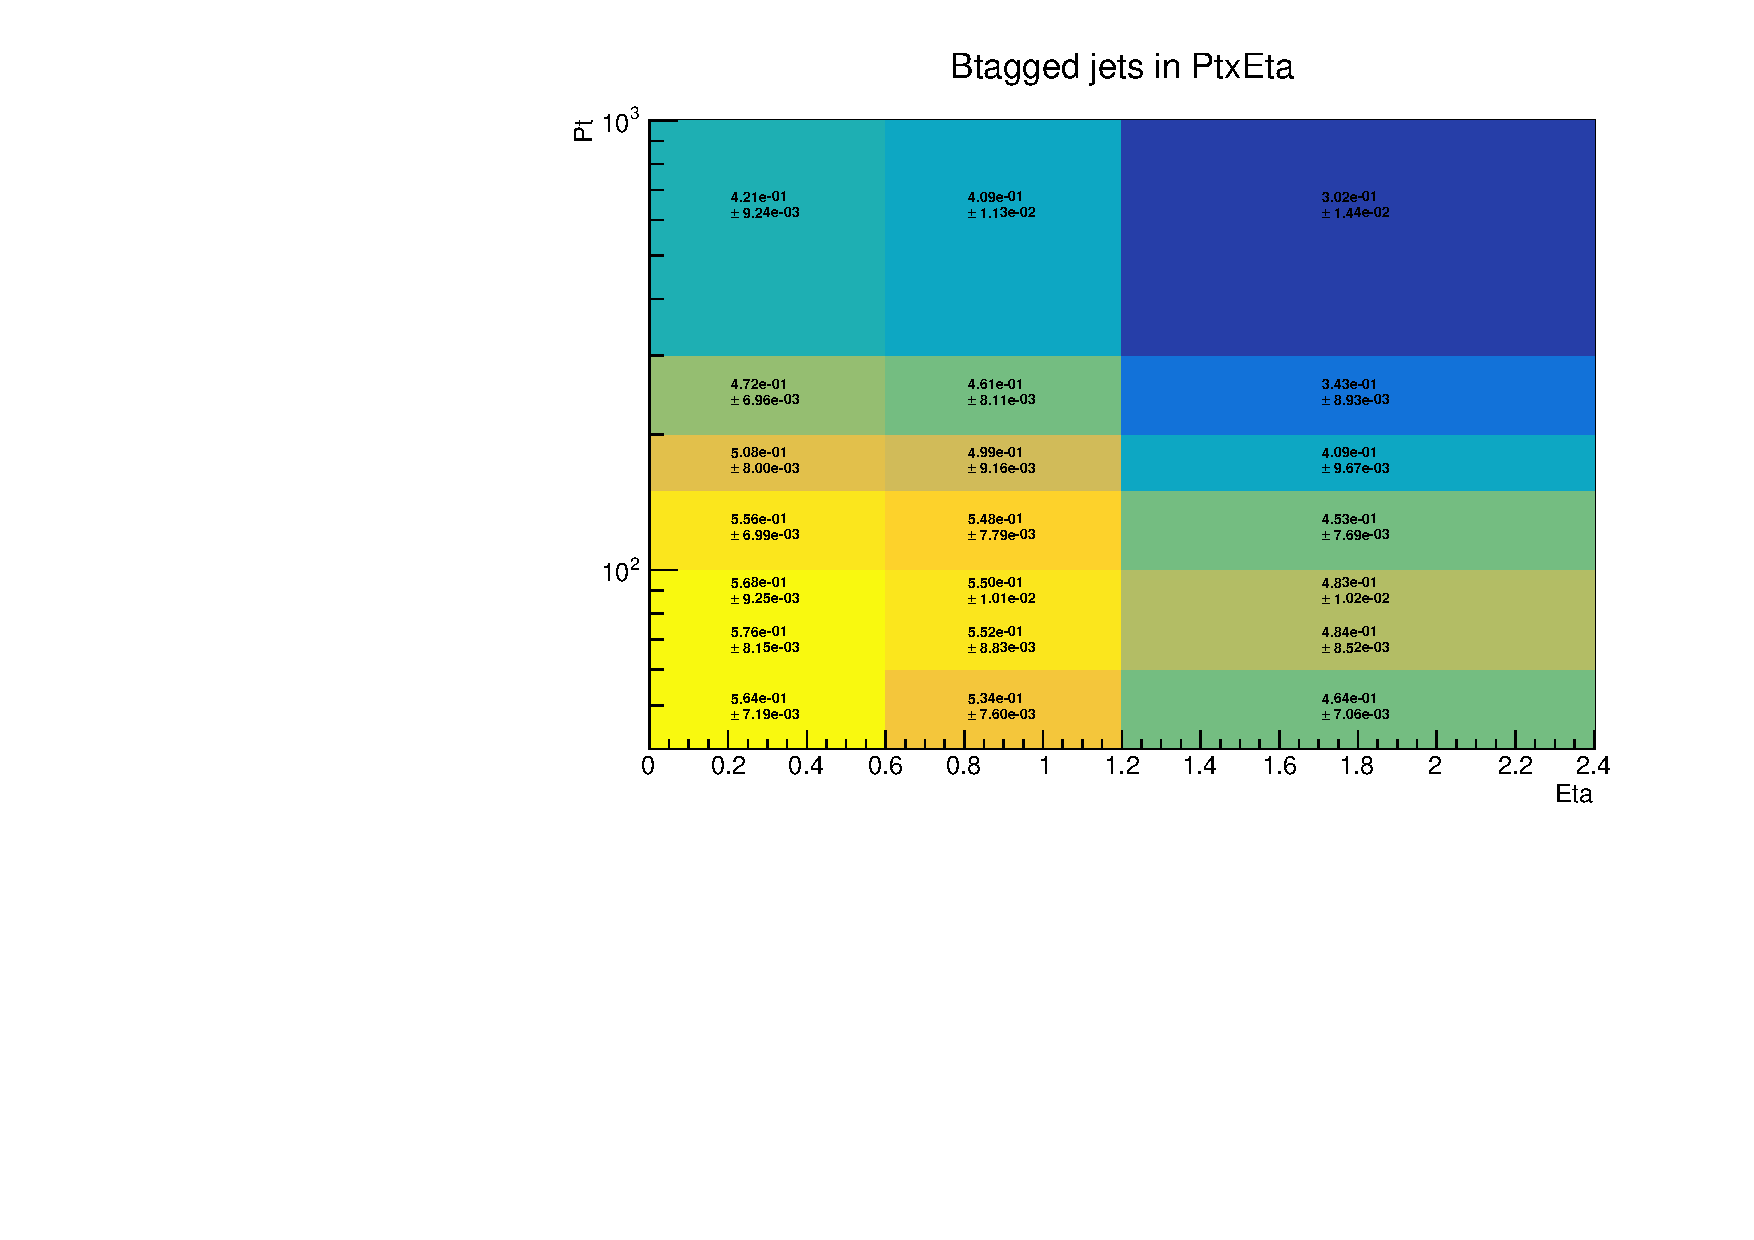
\includegraphics[width=0.45\textwidth]{figures/sec-jets/btageff_tight.pdf}\hfil
  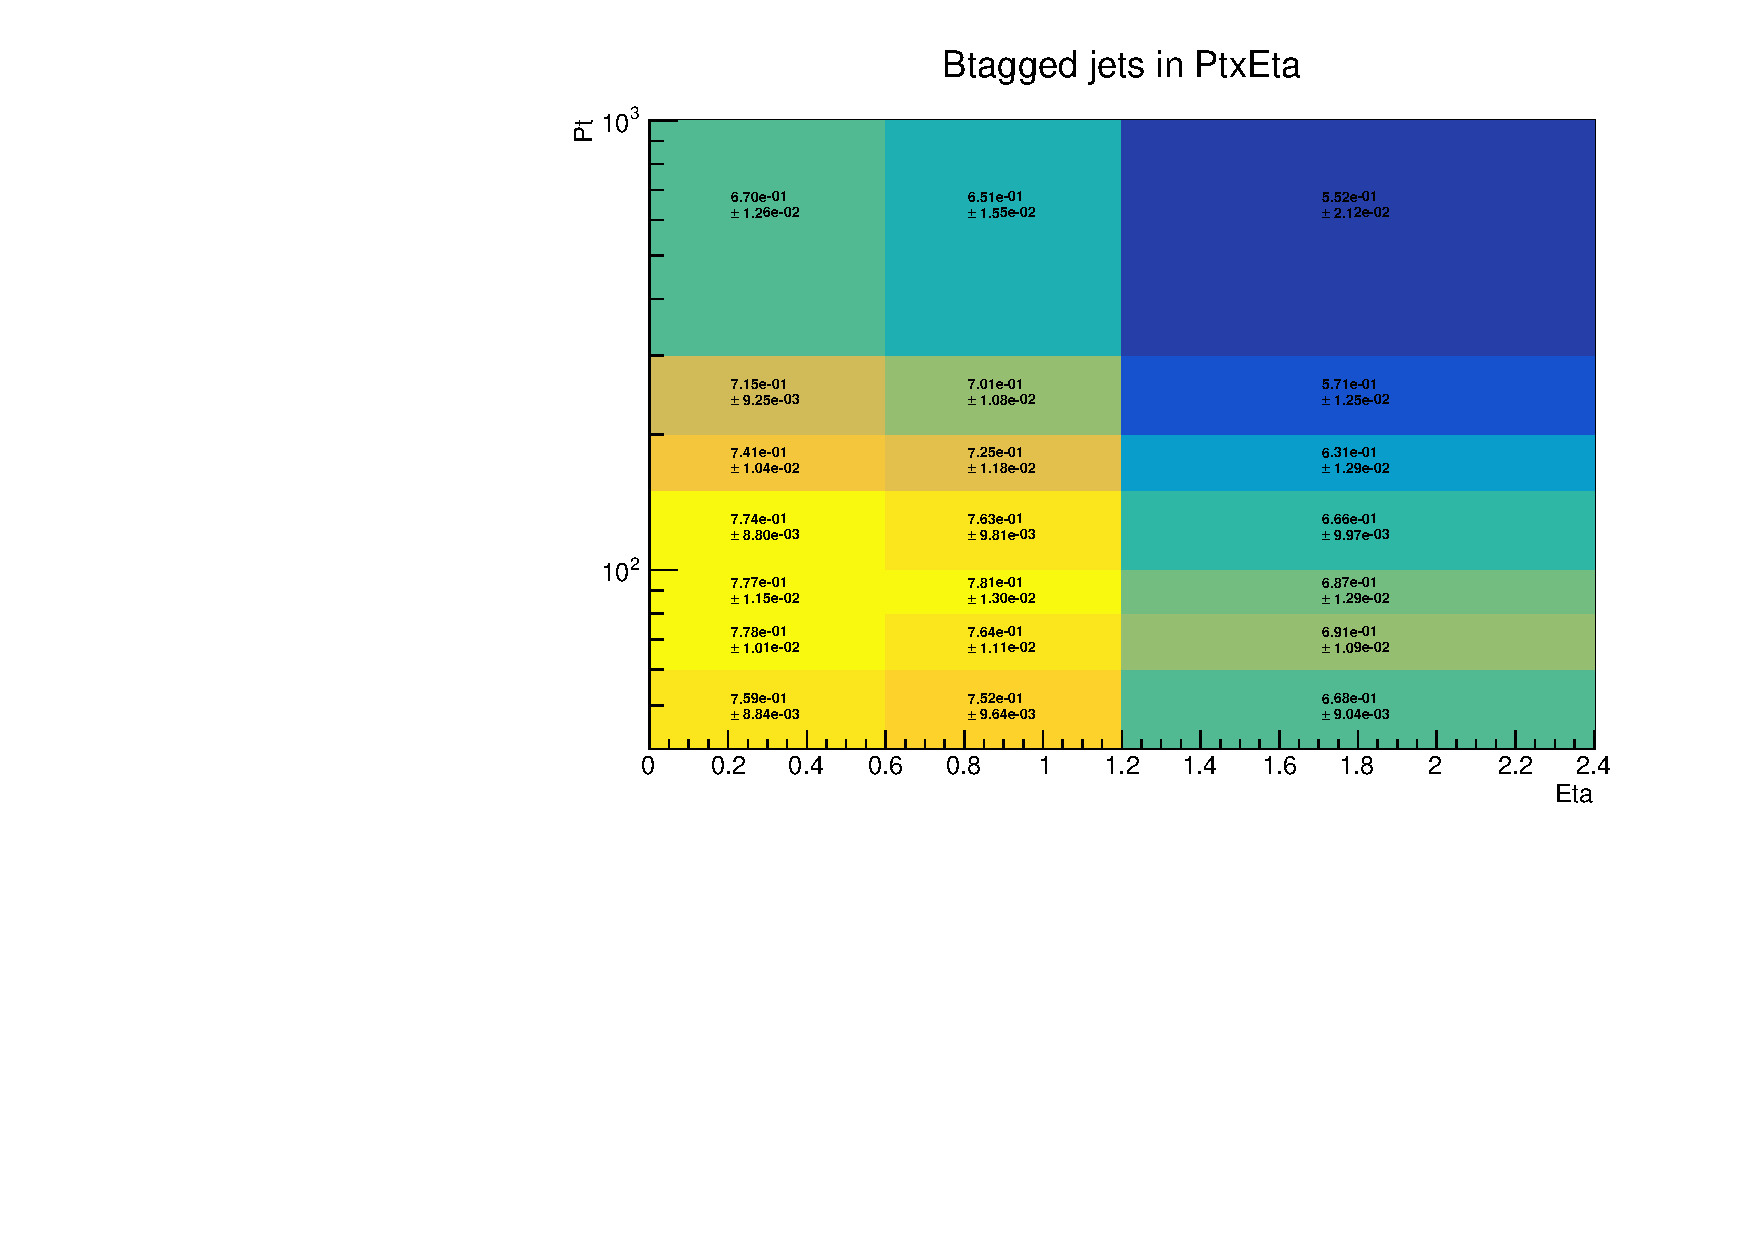
\includegraphics[width=0.45\textwidth]{figures/sec-jets/btageff_medium.pdf}\hfil
  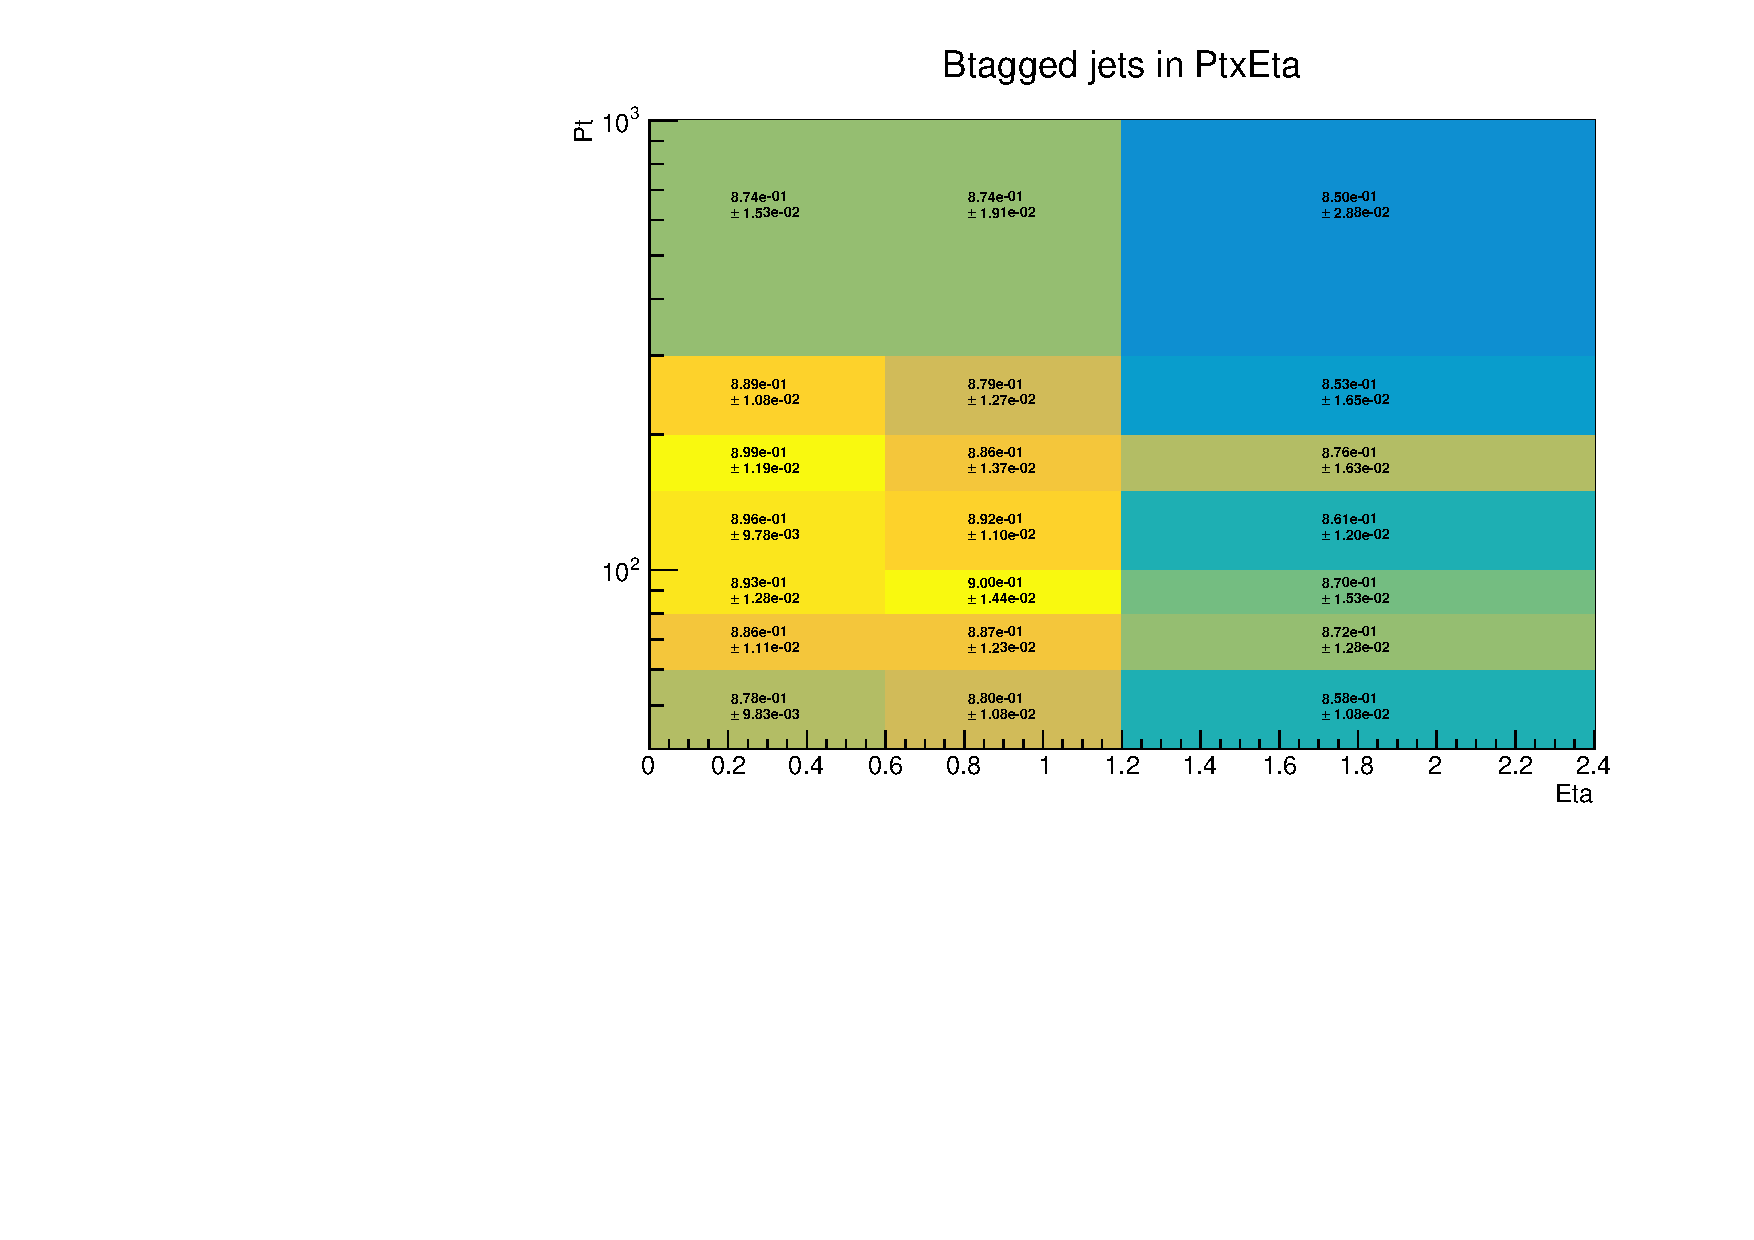
\includegraphics[width=0.45\textwidth]{figures/sec-jets/btageff_loose.pdf}\hfil 
  \caption{B-tagging efficiency for tight, medium and loose working points, as a function of jet $p_{T}$ and $|\eta|$.}
  \label{fig:btageff}
\end{figure*}

